\documentclass[a4paper, oneside]{discothesis}

\usepackage[utf8]{inputenc}
\usepackage[T1]{fontenc}
\usepackage{float}
\usepackage{multirow}
\usepackage{booktabs}
\usepackage{makecell}
\usepackage{tabu}
\usepackage{lmodern}
\usepackage[top=2cm,left=2.2cm,bottom=2cm,right=2cm]{geometry}
%%%%%%%%%%%%%%%%%%%%%%%%%%%%%%%%%%%%%%%%%%%%%%%%%%%%%%%%%%%%%%%%%%%%%%%%%%%%%%%%%%%%%%%%%%%%%%%%%
% DOCUMENT METADATA

\thesistype{Master's Thesis} % Master's Thesis, Bachelor's Thesis, Semester Thesis, Group Project
\title{Performance Gap in Swiss Buildings}

\author{Ying He}
\email{yihe@student.ethz.ch}

\institute{Chair of Building Physics\\[2pt]
ETH Zürich\\[2pt]
Laboratory for Urban Energy Systems\\[2pt]
Empa,Dübendorf\\[2pt]}

% Optionally, you can put in your own logo here
%\logo{
\includegraphics[width=0.2\columnwidth]{figures/disco_logo_faded}}

\supervisors{Dr. Kristina Orehounig\\[2pt] Dr.\ Georgios Mavromatidis\\[2pt]}

% Optionally, keywords and categories of the work can be shown (on the Abstract page)
%\keywords{Keywords go here.}
%\categories{ACM categories go here.}

\date{\today}
\graphicspath{{./figures/}}
%%%%%%%%%%%%%%%%%%%%%%%%%%%%%%%%%%%%%%%%%%%%%%%%%%%%%%%%%%%%%%%%%%%%%%%%%%%%%%%%%%%%%%%%%%%%%%%%%

\begin{document}

\frontmatter % do not remove this line
\maketitle

\cleardoublepage

\begin{acknowledgements}
 I would like to thank my thesis advisors Dr. Orehounig and Dr. Mavromatidis. Whenever I ran into troubles or had a question about my research, the doors to their office are always open and my emails are always replied within short time with solutions. 
\end{acknowledgements}


\begin{abstract}
 	Around 30\% of the world energy are consumed by building sector. Therefore, it is of importance to develop an accurate and efficient approach to estimate the building energy consumption and help improving the current building energy systems. This thesis aims to reduce the deviation between calculated and measured heating demands and find the short-comings in SIA 380/1 calculation method. In addition, this thesis also aims to validate a number of factors which are thought to have great impacts on building energy consumption, and to find out some important factors which are neglected in SIA 380/1 standards. A residential building and an office building are firstly accurately modeled and calculated using EnergyPlus and SIA 380/1 standard. Then, both buildings are  calibrated based on historical annual heating demand and hourly indoor temperature, then several key building parameters are modified within a certain range given by both SIA 2024 Norm and experience values. Based on a large number of simulations, the result indicated that the most influential parameters in simulation are outdoor environments, key area temperature heating setpoints, external wall solar absorptance, infiltration and installed lighting capacity and schedule. In order to reduce the performance gap, it is recommended to create an accurate building envelope with accurate construction material properties and air-tightness, as well as a close-to-reality assumption on user behaviors and indoor environment, and apply a representative outdoor environment.
\end{abstract}

\tableofcontents

\mainmatter % do not remove this line

% Start writing here
\chapter{Introduction}
	Building simulation are widely used for different purposes such as to benchmark buildings or to evaluate energy demands and indoor thermal comfort. However, due to a number of factors, there are often deviations between calculated  and measurement values, a phenomenon which is called \textbf{performance gap}. Previous studies which used a standardized method \textbf{SIA 380/1} to calculate the heating demand of several buildings observed considerably large performance gaps in uninsulated buildings as shown in Figure \ref{fig:SIA380PG} \cite{SIAPreviousreport}. It is believed that part of the problem come from a non-accurate calculation method and non-realistic assumptions on some building parameters and outdoor environment \cite{SIAPreviousreport}. \\

	
	Therefore, the purpose of this thesis is to find out the main causes of the performance gap in uninsulated buildings, as well as the most influential factors and input assumptions in building simulation. In addition, this thesis also aims to investigate how the resulting energy demand variations affect the performance gap.\\


	Two uninsulated buildings, one residential and one office buildings, are carefully modeled and analyzed using different approaches including static calculation (SIA 380/1) which based on monthly average inputs, and dynamic simulation (EnergyPlus) which based on hourly timestep inputs initiative calculation method \cite{SIAPreviousreport,SIA2024Shop,crawley2000energy}. The buildings are firstly calibrated to match the historical measurement, then model input parameters are modified and the most influential factors can be identified.\\

		\begin{figure}[!ht]
		\centering
		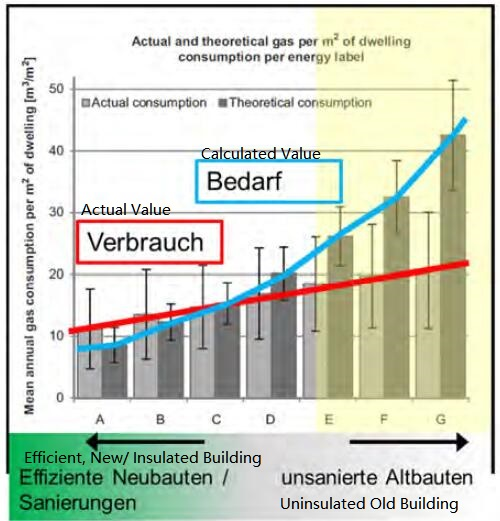
\includegraphics[scale=0.65]{SIA380Issue.jpg}
		\caption{SIA380/1 Calculation Performance Gap Indicator \cite{SIAPreviousreport}}
		\label{fig:SIA380PG}
		\end{figure}
%\TODO{This is a TODO annotation.}


\chapter{Literature Review}
	Over the past years, there is a large number of research paper about the building energy performance gap (BEPG). Performance gap can cause problems in energy management system as they provide inaccurate information to upstream energy suppliers or waste investments in buying over-capacity or under-capacity equipment. However, the root cause of this gap is not clearly identified, and the gap can not be effectively managed and eliminated \cite{FREI2017421}.\\
	
	According to a recent review about the building energy performance gap by Zou et al.\cite{ZOU2018165}, most of these research papers on the topic of performance gap would contain one or more of the following 5 elements: (1) building type, which can be classified into different groups such as residential, office, commercial, or even more specific types such as single-family house, multi-family house, shopping mall, hospital, prison, etc; (2) strategies for closing performance gap, which focus about design concept and technology dependent method (3) building life cycle, which analyses the cause of performance gap in different stages of a building; (4) energy-related stakeholders, whose behavior would affect the performance gap; (5) the influence factors or building parameters that would cause or affect the performance gap \cite{FREI2017421,ZOU2018165}.\\
	
	\textbf{Formation of Performance Gap}\\
		Most causes of performance gap can be grouped into 3 categories base on the stages in the building life-cycle. They are design and simulation problems, construction quality and technology-related problems by contractors and unexpected behaviors of building users \cite{userevaluations,NIU2016275}. These three categories are analysed below:\\
		
		\textbf{(1) Design and simulation problems}\\
		Firstly, in most cases, building designers account for the wrong aspects in design and simulation processes. These include wrong assumptions and predictions about their design such as inaccurate building unheated area's temperature, wrong representation of user behavior, and wrong forecast of outdoor conditions \cite{NIU2016275,HOFFMANN201731}. Also, it is difficult to predict the future environment such as climate, weather, and solar activities, which can lead to huge performance gaps \cite{DIAZ2017393,doi:10.1080/19401493.2012.718797}. For example, rainfall would greatly increase the heat convection coefficient of building facade surface, and therefore increase heat exchange rate through the building envelope \cite{DIAZ2017393}. In addition, due to a difference between labotary environment and site environment, the performance of building materials or technologies in actual use is usually not the same as the lab test value. For example, a 5\% efficiency PV panel would be less than 5\% efficiency if covered with dusts or snow. Therefore, designers usually overestimate the actual performance of some innovated new building material or building control technologies and apply inappropriate assumptions about user behaviors \cite{DEWILDE201440}. \\

		\textbf{(2) Contractors}\\
		Secondly, construction practicers are also a cause for performance gaps. Low quality constructions lead to diviations between the actual building quality and the designed building quality. Poor building quality and poor workmanship will usually reduce the thermal performance and therefore change the building envelope from its designed state. For example, a room with less air-tightness than its design value would require more energy to maintain indoor comfort, and therefore consumes more energy than its designed and simulated results. Additionally, performance gap can be caused by contractors when they use improper construction techniques and when they are unable to discover hidden problems such as thermal bridge or small cracks due to time and budget constraints \cite{DEWILDE201440}. In some cases, these problems would lead to huge building parameter deviations and alter the building energy consumptions from the design value and create performance gaps \cite{FREI2017421,DEWILDE201440}.\\ 

		\textbf{(3) User Behaviors}\\
		Lastly, as the last and main stage of building's life-cycle, different behaviors of building users are also important sources of performance gap \cite{ZOU2018165}. These behaviors, either deliberate or unconscious, are usually not the optimum ways to operate a building. Building owners or occupants have specific behaviors due to their social and personal characteristics, attitude, experience, and thermal comfort standard \cite{userevaluations,LAWRENCE2016651}. For example, users may leave unnecessary appliance on without notice or open the windows when heatings or cooling system is operating \cite{FREI2017421}. Therefore, if an ideal user behavior is used in the building simulations, the input value may not accurately represent the actual user behavior, and the simulation result will not accurately reflect the actual energy consumption and create a performance gap.\\

	\section{Strategies For Closing Performance Gap} 
		When the causes of performance gap are found out, strategies for closing the gap can also need to be developed. These strategies are grouped into 2 categories, which are design concept and technology \& methods \cite{ZOU2018165}.

		\subsection{Design Concept}
			\textit{Passive design} is thought to be able to eliminate or decrease the impact of user behavior on energy consumption. Its philosophy is that if a building is designed in a way that no active equipment is needed, user behaviors would not influence the passive mechanism \cite{BLIGHT2013183,NORFORD1994121}. However, this approach has high construction quality requirements and can only have positive effects when both building designers and the occupants fully understand the building energy system. If building designers have inaccurate information about occupants, or building constructors do not have the capability to construct the building according to the specifications, or if the occupants do not fully understand the building system, passive design approach can only have adverse impacts \cite{ZOU2018165}.\\

			\textit{Active design}, on the other hand, use building automation system to improve occupants' thermal comfort and hopefully reduce the chance of wrong operations by occupants. Same as passive design, this design approach also require high quality equipment and construction team, and a comprehensive understanding of buildings and occupant behaviors to function well \cite{DEWILDE201440}.\\

			\textit{Human-in-the-loop} is another approach that requires human interaction \cite{karwowski2001international}. As information is a critical factor in building energy, the more comprehensive and accurate the obtained data, the more precise the result would become \cite{NIU2016275}. Therefore, in order to improve the accuracy of "human-in-the-loop design", is of importance to collect accurate data. There have been research which used advanced technology such as genetic algorithm, machine learning, virtual reality technology and augment reality technology to collect building data for simulations and calculations \cite{karwowski2001international}. The limitations of this approach would be the difficulty to collect comprehensive human information, and there is an uncertainty of occupant behaviors and different occupants may influence each other \cite{masoso2010dark}.

		\subsection{Technology and methods (T\&M)}

			It is believed that using more advanced and innovative technologies and calculation methods would help closing the performance gap \cite{ZOU2018165}. Previous research has grouped most technologies and methods into 4 categories, namely T\&M for calculating energy consumption, T\&M for energy related data collection and analysis, T\&M for occupant behavior modeling and simulation and T\&M for energy system controlling \cite{ZOU2018165}.\\

			\textit{(1) T\&M for calculating energy consumption} can be further divided into \textit{Black box} methods, \textit{Grey box} methods, and \textit{White box} methods. A black box method, such as genetic algorithm and artificial neural networks, calculates energy consumption without physical knowledge. The white box method, such as \textit{EnergyPlus, DOE-2, Ecotect} calculation engines, calculates energy consumption based on the thermodynamic behavior of the building and its occupants \cite{li2014methods,xu2007optimal}. The grey box method is a combination of the black and white box method, in hope of eliminating the limitations of both methods \cite{ZOU2018165}.\\

			\textit{(2) T\&M for data collection and analysis} 
			focuses on obtaining and utilizing the occupant behavior and building operation information \cite{ZOU2018165}. Similarly, T\&M for data collection and analysis can be divided into two approaches, namely \textit{post occupancy} data collection and \textit{pre-occupancy} data collection \cite{ZOU2018165}. \textit{Post-occupancy data collection} is the traditional and most commonly used data collecting approach, which uses different sensors and monitors to record occupants' activities as shown in Figure \ref{fig:Energy_DataCollection} below. However, since all buildings are more or less different from each other, post-occupancy data collection would not provide a customized and future-oriented prediction of a newly designed building, neither would it explain the reasons behind certain occupant behaviors \cite{NIU2016275}.\\

			To overcome this limitation, \textit{pre-occupancy data collection} is developed to collect virtual occupancy behavior data based on VR or BIM building models. By this approach, customized occupancy data can be collected and designers can also improve the building design based on the collected virtual occupancy data. However, this method is not flawless, as the virtual occupancy behavior would likely be different from the actual behaviors in the real buildings.\\


			\begin{figure}[h!]
			\centering
			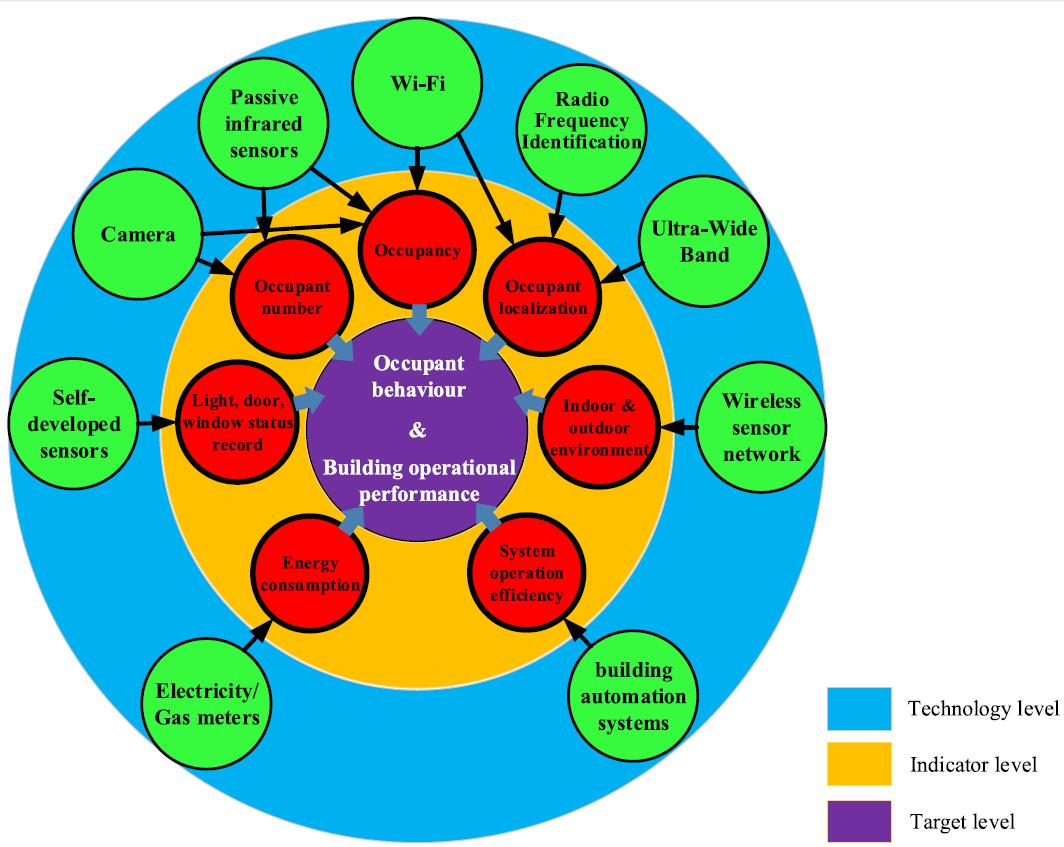
\includegraphics[scale=0.5]{Energy-relatedData.jpg}
			\caption{Technology and method for energy-related data collection \cite{jia2017occupancy}}
			\label{fig:Energy_DataCollection}
			\end{figure}

			\textit{Statistical analysis} is mostly used to develop a numerical relationship among energy consumption, outdoor environment, indoor environment and comfort, occupant behavior and other information using statistical tests, regression analysis and curve fitting \cite{ZOU2018165}. Previous research also show that the above mentioned data collection approaches would be slow and expensive, and the collected data volume is massive and unstructured \cite{liang2016occupancy}.\\

			In order to process this massive amount of data, \textit{Data mining} would be a good technology to structure the collected data and find out the unknown correlations between different data sets. Currently, data mining is used to analyze building energy consumption data and occupancy/occupant behavior data \cite{xiao2014data}.\\

			\textit{(3) T\&M for occupant behavior modeling and simulation}\\
			As building occupants are capable to greatly alter the building indoor environment, it is of importance to know how exactly did they operate the building when a building is subjected to energy analysis or building simulations. However, obtaining an exact set of occupant activity record through the simulation period is hardly possible for most cases. Therefore, some technologies and methods are developed to generate a reasonable set of occupant behavior. \textit{T\&M for occupant behavior modeling and simulation} are mainly two groups, namely \textit{agent-based modeling (ABM)} and \textit{stochastic process modeling} \cite{ZOU2018165}.\\

			\textit{Agent-based modeling (ABM)} simulates the actions and interaction of agents, such as individual, group or equipment, and investigate how they interact with the whole system \cite{jia2017occupancy}. Some previous studies have used ABM to address the interrelation between different occupants, or to simulate user-defined social constraints from other occupants on an agent's certain behavior. The advantage of ABM is its potential capability to integrate with energy simulation program and its capability to deal with interactions and uncertainties \cite{ZOU2018165}. However, the limitation of ABM is not negligible. Currently, ABM are more dependent on assumptions rather than actual data, and it is difficult to verify a model based on ABM \cite{ZOU2018165,jia2017occupancy}. \\


			As the occupant behavior is more or less random, \textit{stochastic modeling} can be widely used in many researches involing estimating probability distributions of occupant behavior. In most cases, stochastic process modeling approach focus on relatively long-term occupancy prediction or classification instead of a certain behavior at a certain time \cite{ZOU2018165}.
			In this thesis, stochastic process modeling approach based on SIA standards is used in the dynamic energy analysis part, the detailed parameters can be found in chapter methodology.\\

			\textit{(4) T\&M for energy system controlling} aims at reducing building energy consumption without sacrificing the occupants' thermal comfort, and can be devided by three groups: \textit{intelligent HVAC system, artificial lighting} and \textit{occupancy-based control system} \cite{ZOU2018165,hong2015review}. The limitation for T\&M for building automatic control would be it relies heavily on controlling algorithms and the accuracy of sensoring equipments. Therefore, a mal-functioning sensor group would paralise the control system.

	\section{Building Simulation Parameter Variation}
		There are a number of research papers trying different approaches to mitigate the problem caused by input uncertainties due to lack of necessary information \cite{GeorgeThesis}. A majority of research papers involve using normal distribution to allocate the uncertain parameters while some others also use different allocation methods such as triangular or uniform distribution. Most uncertainties can be grouped into different types, Mavromatidis \cite{GeorgeThesis} has provided a summary of building simulation uncertainties and classified the related simulation parameters into 4 different types: (1) Building-related parameters; (2) occupant-related parameters; (3) indoor environment-related parameters and (4) weather/climate parameters \cite{GeorgeThesis}.\\

		(1) \textit{Building-related parameters} are those related to building envelope material properties such as construction material thermal properties and infiltration/air tightness. The uncertainties of this type of parameters are due to unknown or partly unknown construction information, or because of the material performance being inconsistent with the lab specifications due to measurement errors, poor workmanship, installation, quality and aging problem \cite{GeorgeThesis}. One of the most difficult-to-measure parameters is air-tightness/air infiltration rate, which can be measured only by a time-consuming blower-door test. Therefore, in many cases a typical assumed value is used for the building simulation processes, and this typical assumed air infiltration value is sometimes different from the actual value \cite{GeorgeThesis,burhenne2013uncertainty}.\\

		(2) \textit{Occupant-related parameters} are the parameters relevant to occupants' presence and activities such as occupancy patterns and usage of lighting, electronic appliances, and domestic hot water consumption. As discussed in previous chapters, user behaviors are essentially random and can greatly influence the indoor environment. Therefore, the deviations in occupant-related parameters can sometimes lead to huge performance gap or indoor environment variations \cite{GeorgeThesis}. To improve this, using ``typical schedules'' is a simple way to address the different occupant working patterns. Yao and Steemers \cite{yao2005method} has purposed 5 typical household occupancy schedules for different working patterns such as full-time commuter, part-time, and unemployed/in-house occupants. Silva and Ghisi \cite{silva2014uncertainty} also purposed 3 different lighting schedules for different utilisation hours.\\

		(3) \textit{Indoor environment-related parameters} such as thermostat values, ventilation level, shading and window opening preferences can be varied from person to person. Similar to the user behavior pattern discussed above, probabilistic approaches are widely used in several researches \cite{GeorgeThesis} Both thermostat setpoints and indoor air quality such as air change rates are of high interest for many researchers, and normal and triangular distribution are a popular way to address uncertainties related to these indoor environment-related parameters \cite{GeorgeThesis}. 

	\section{Building Simulation Research for Swiss Buildings}
		In 2015 a research has been done by \textit{Lemon Consult} \cite{SIAPreviousreport} aiming to investigate the reason behind the huge performance gaps in uninsulated old buildings when using SIA 380/1 and SIA 382 calculation method. The research concluded that three main reasons are the most important: too poor U-values, too low indoor air temperature for unheated ares (based on a research on basement actual temperature), and the discrepancies between standard climate data and actual outdoor air temperature \cite{SIAPreviousreport}. However, there are still some unsolved problems in the previous research. Firstly, the actual temperature of the building site is not fully recorded and used in SIA 380/2 calculation. Secondly, the relations and rankings between the key parameters are not clear. Therefore, in this thesis, a more accurate and up-to-date weather information is implemented in both static and dynamic calculations, and the correlation relationship between the heating demand and each key parameter are also investigated more closely.



\chapter{Methodology}
	In order to achieve the thesis aim to reduce the deviation between calculated and measured heating demands and find the short-comings in SIA 380/1 calculation method, the research of this thesis research is divided into three parts. In the first part, a 3D model with exact geometry and orientation for each building is built using \textit{DesignBuilder (version4.7)}. In the second part, the two buildings are subject to building energy analyses using both SIA 380/1 standard tool and EnergyPlus. The models are then verified and calibrated by comparing the measured historical indoor temperature with the calculated indoor temperature. In the final part, a set of key building parameters are varied with a certain range. A number of building models with different building parameters are subject to analyses using jE-Plus. Further analyses would identify the correlation between parameters as well as the influence of climate data. Figure \ref{fig:overview} below shows the key approaches to achieve the thesis aim.\\

		\begin{figure}[ht]
		\centering
		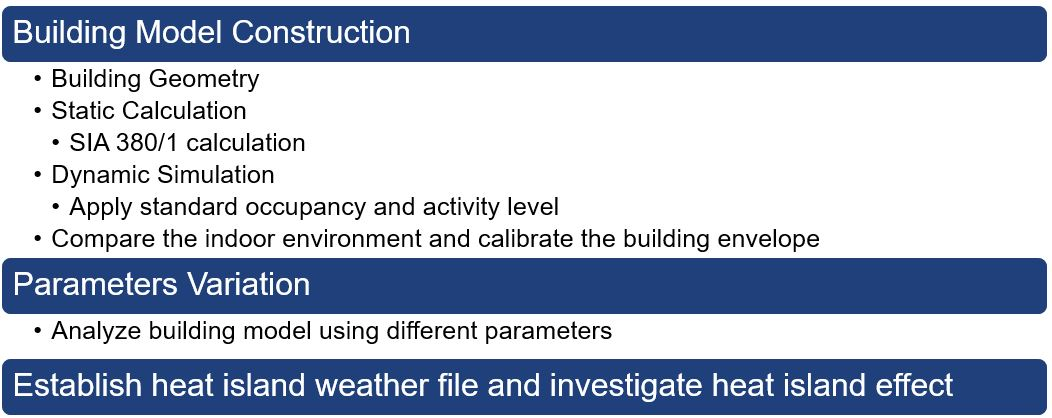
\includegraphics[scale=0.5]{overview.JPG}
		\caption{An overview of the methodology}
		\label{fig:overview}
		\end{figure}

	\section{Office Building Introduction}
		

		 
		
		According to the given information, the office building is constructed in 1951 and is located at Sumatrastrasse 10, 8006 Zurich, Switzerland. The building has 4 floors and a basement. The building  is facing west, and the window-to-wall ratio is 59\% on its west and south facade. The east facade of its ground floor and first floor is submerged into ground and there are heavy cover of plants on the upper floors with only a few necessary windows. There is also an underground floor used as warehouse and it's not included in any building model in this thesis.\\

		Figure \ref{fig:sumatra_og2} and \ref{fig:sumatra_og3} below are the floor plans of the building.
		The floor layout of ground floor, first floor and second floor are thought to be identical, and the third would have some small differences. For each floor, there is a toilet, a small office and 2 middle offices and a staircase. There is also a big office in each floor at the south side at ground floor, first floor and second floor. At the third floor, part of the big office and the corridor become a meeting room and a small pastry area as shown in the figures below. The detail building envelope material and modelling parameters are at chapter \textit{Methodology}.

		\begin{figure}[ht]
		\centering
		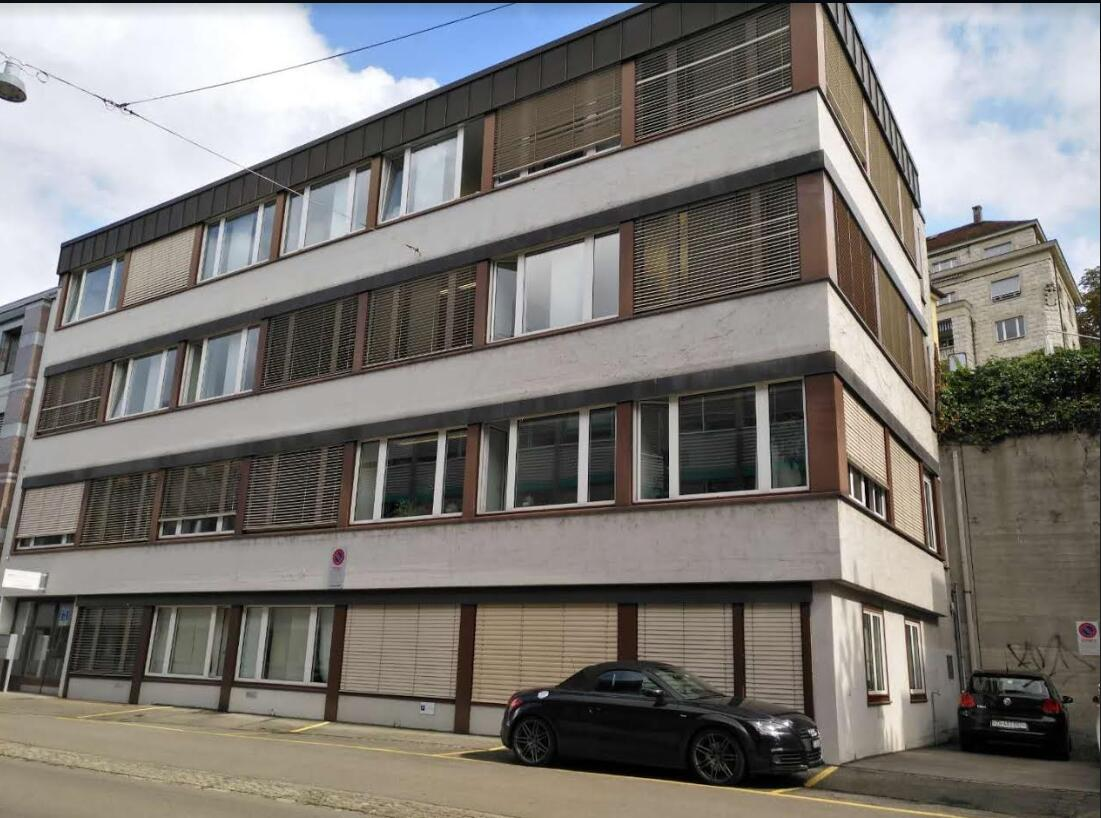
\includegraphics[scale=0.45]{Sumatra_photo.jpg}
		\caption{Sumatrastrasse 10 Office Building}
		\label{fig:Sumatra_photo}
		\end{figure}
		
		\begin{figure}[ht!]
		  \centering
		  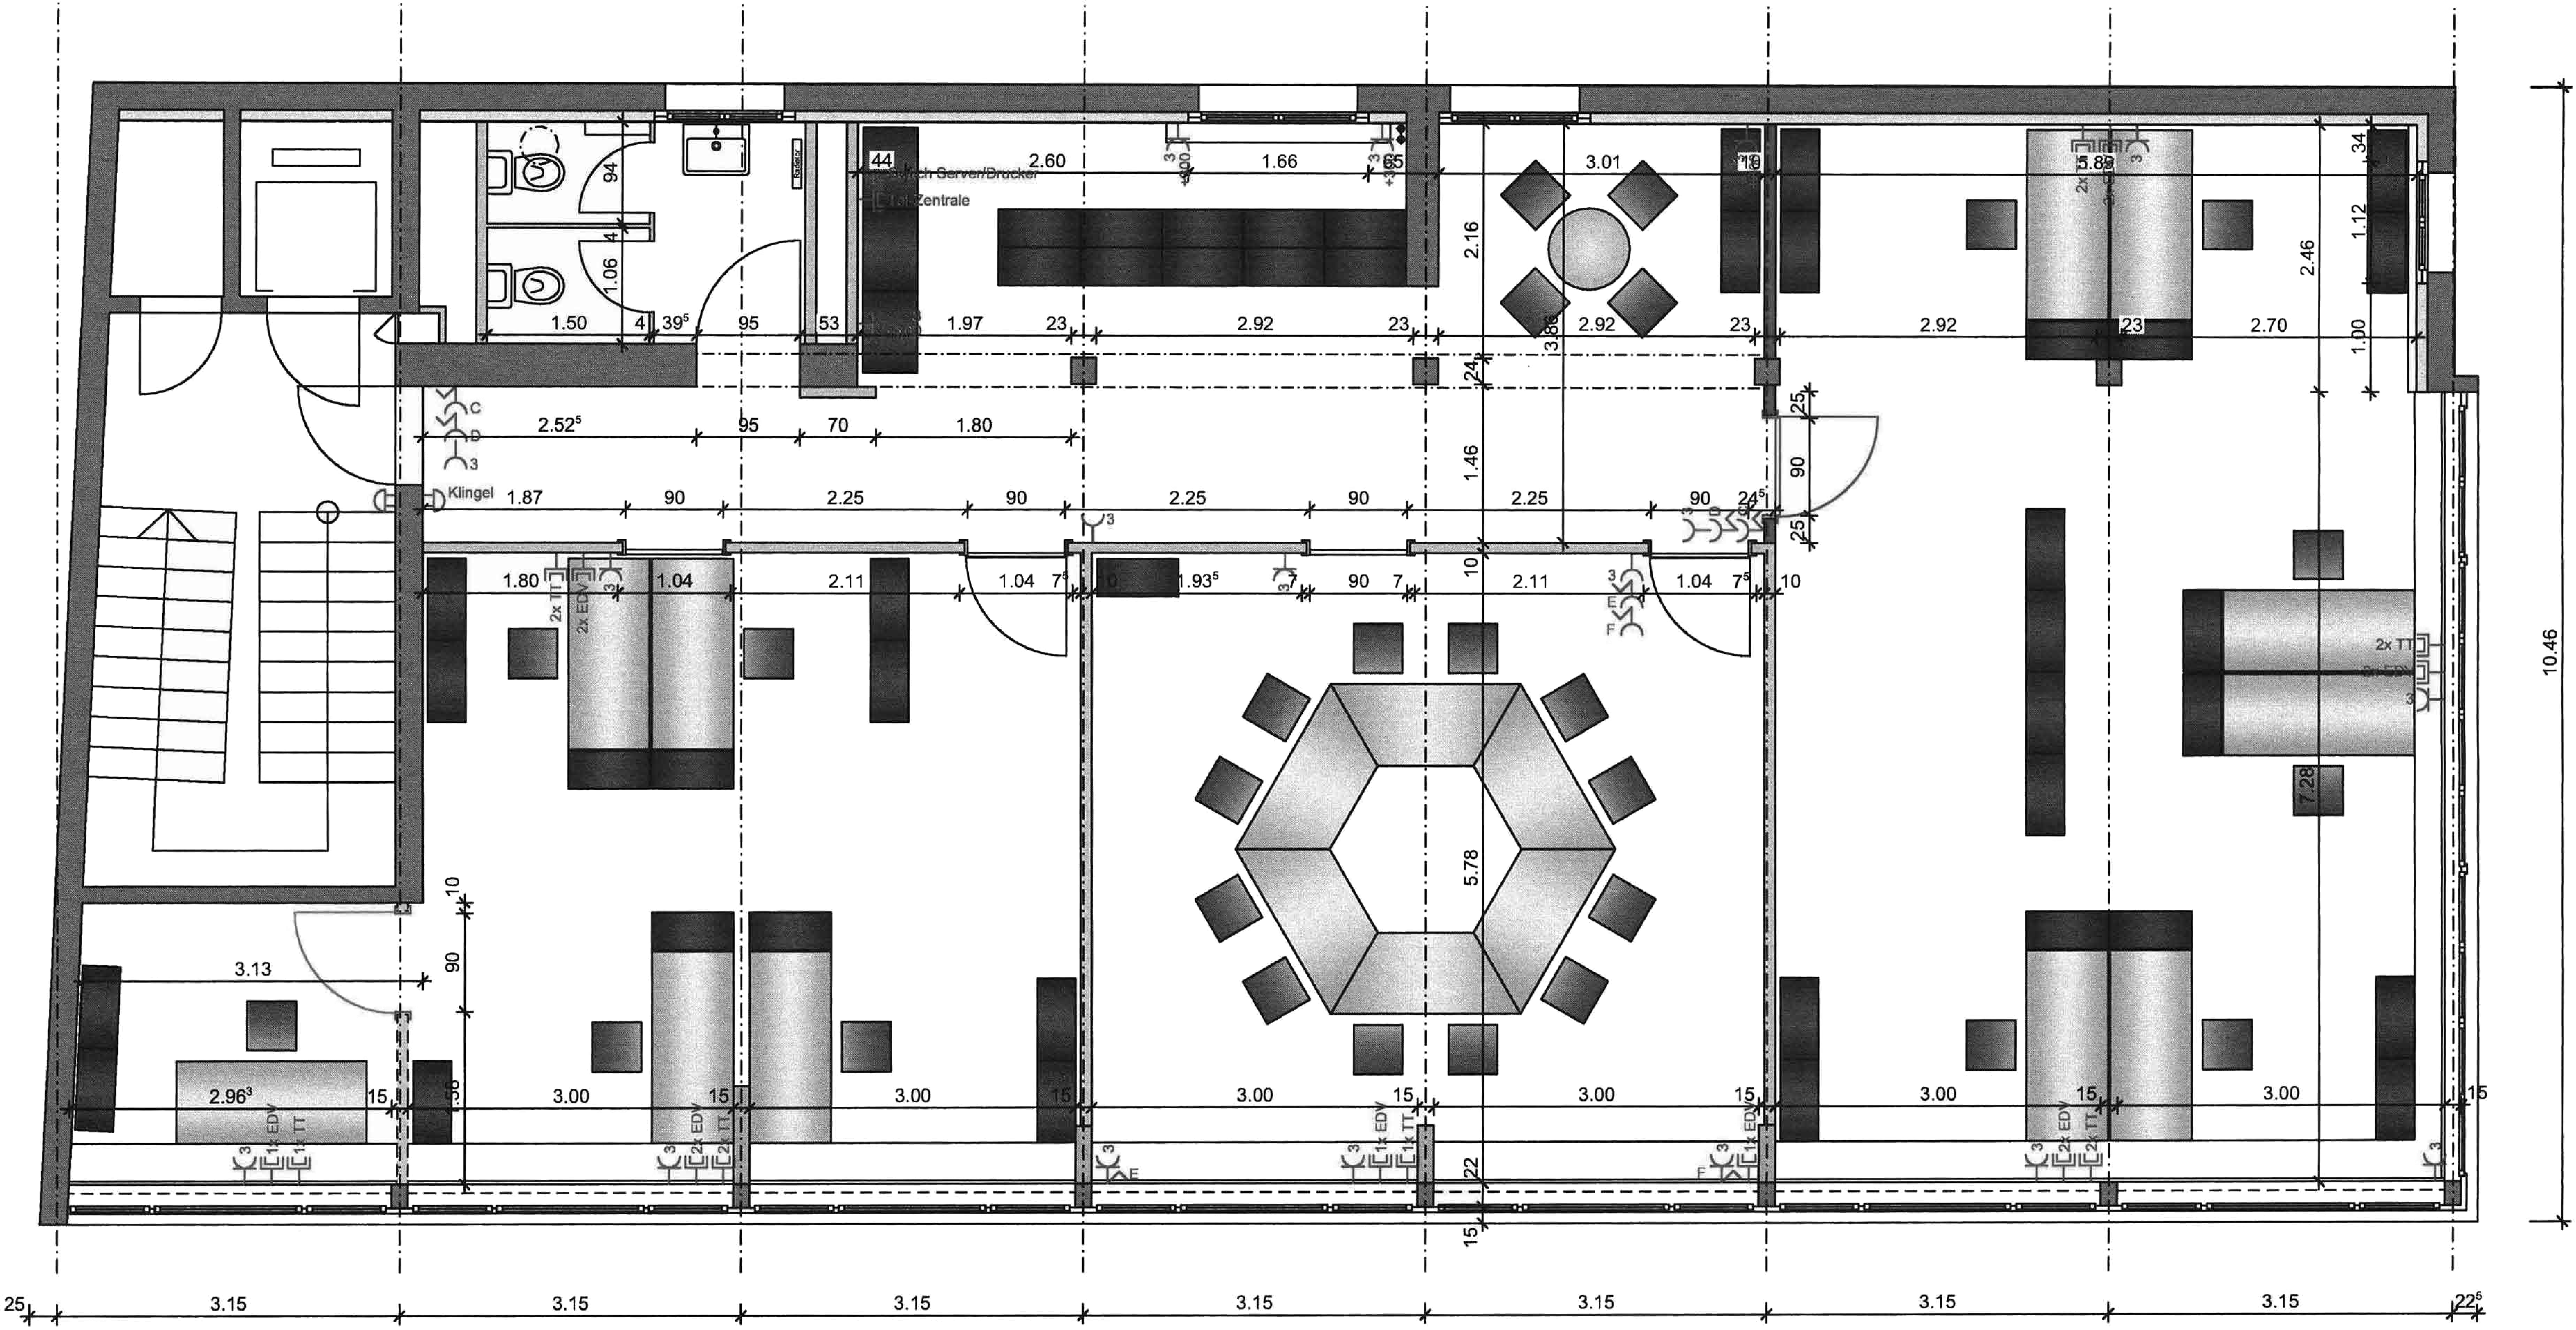
\includegraphics[scale=0.12]{Sumatra_OG2_Plan.pdf}
		  \caption{Floor plan of office building (Sumatra) ground floor to 2$^{nd}$ floor}
		  \label{fig:sumatra_og2}
		 \end{figure}

		\begin{figure}[ht!]
		  \centering
		  \includegraphics[scale=0.12]{Sumatra_OG3_Plan.pdf}
		  \caption{Floor plan of office building (Sumatra) 3$^{rd}$ floor}
		  \label{fig:sumatra_og3}
		\end{figure}
	
	\newpage	
	\section{Residential Building Introduction}
		Figures \ref{fig:hongg_NE} and \ref{fig:hongg_SW} show photos of the residential building. The residential building is a part of a multi-family town house constructed in 1894. It is located at Honggerstrasse 23, 8037 Zurich, Switzerland. The building has 5 floors, the top floor is a loft and there is also an extra basement. There are 4 apartments in the building. The first apartment occupies the ground floor and the first floor, and the other 3 apartments each occupy one floor. Figure \ref{fig:hongg_eg_plan} and Figure \ref{fig:hongg_og1_plan} are the floor plans of the residential building. The ground floor is connected with the first floor internally via a small staircase behide the kitchen. The black and red lines in Figure \ref{fig:hongg_eg_plan} show the ground floor layout and the yellow line indicates the layout of the upper floor. Similarily, Figure \ref{fig:hongg_og1_plan} shows the floor plans from first floor upward. The  red line indicates the layout of first floor and the yellow line shows the layout from second floor up. The detail building envelope material and modelling parameters are shown at \textit{the Chapter Methodology}.\\
		

		\begin{figure}[htbp]
		\centering
		\begin{minipage}[t]{0.48\textwidth}
		\centering
		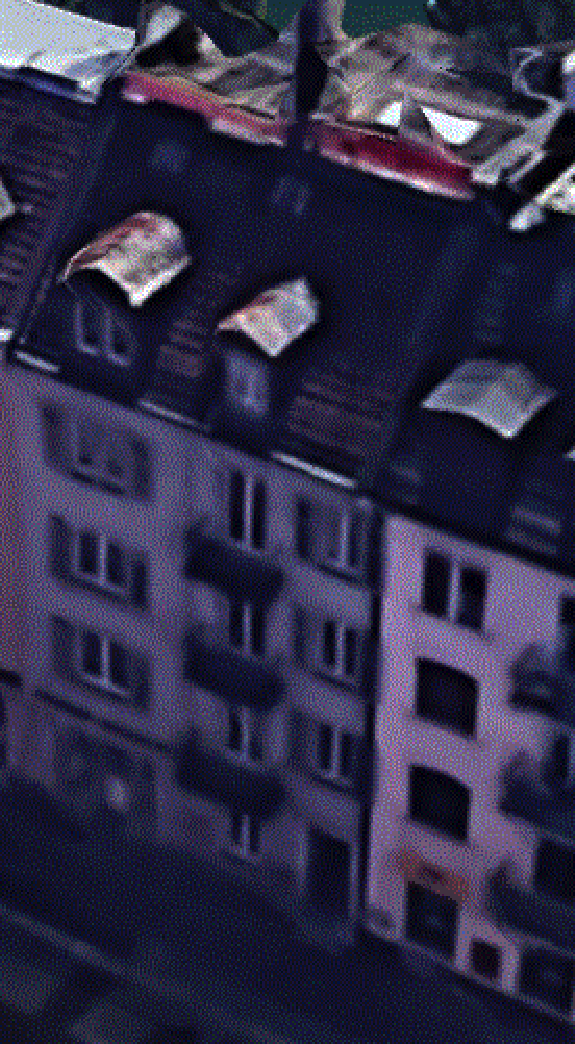
\includegraphics[width=5cm]{Hongg_photo1.pdf}
		\caption{Honggerstrasse 23, NE Side}
		\label{fig:hongg_NE}
		\end{minipage}
		\begin{minipage}[t]{0.48\textwidth}
		\centering
		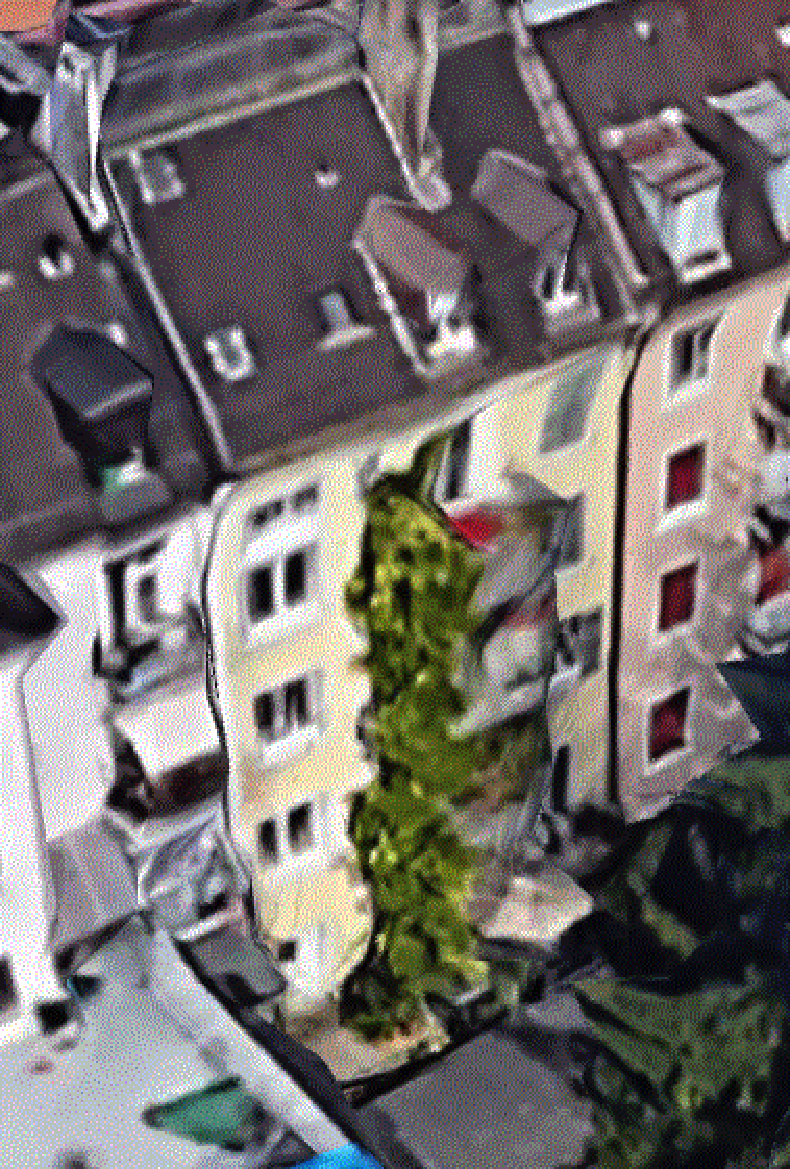
\includegraphics[width=6cm]{Hongg_photo0.pdf}
		\caption{Honggerstrasse 23, SW side}
		\label{fig:hongg_SW}
		\end{minipage}
		\end{figure}

		\begin{figure}[htbp]
		\centering
		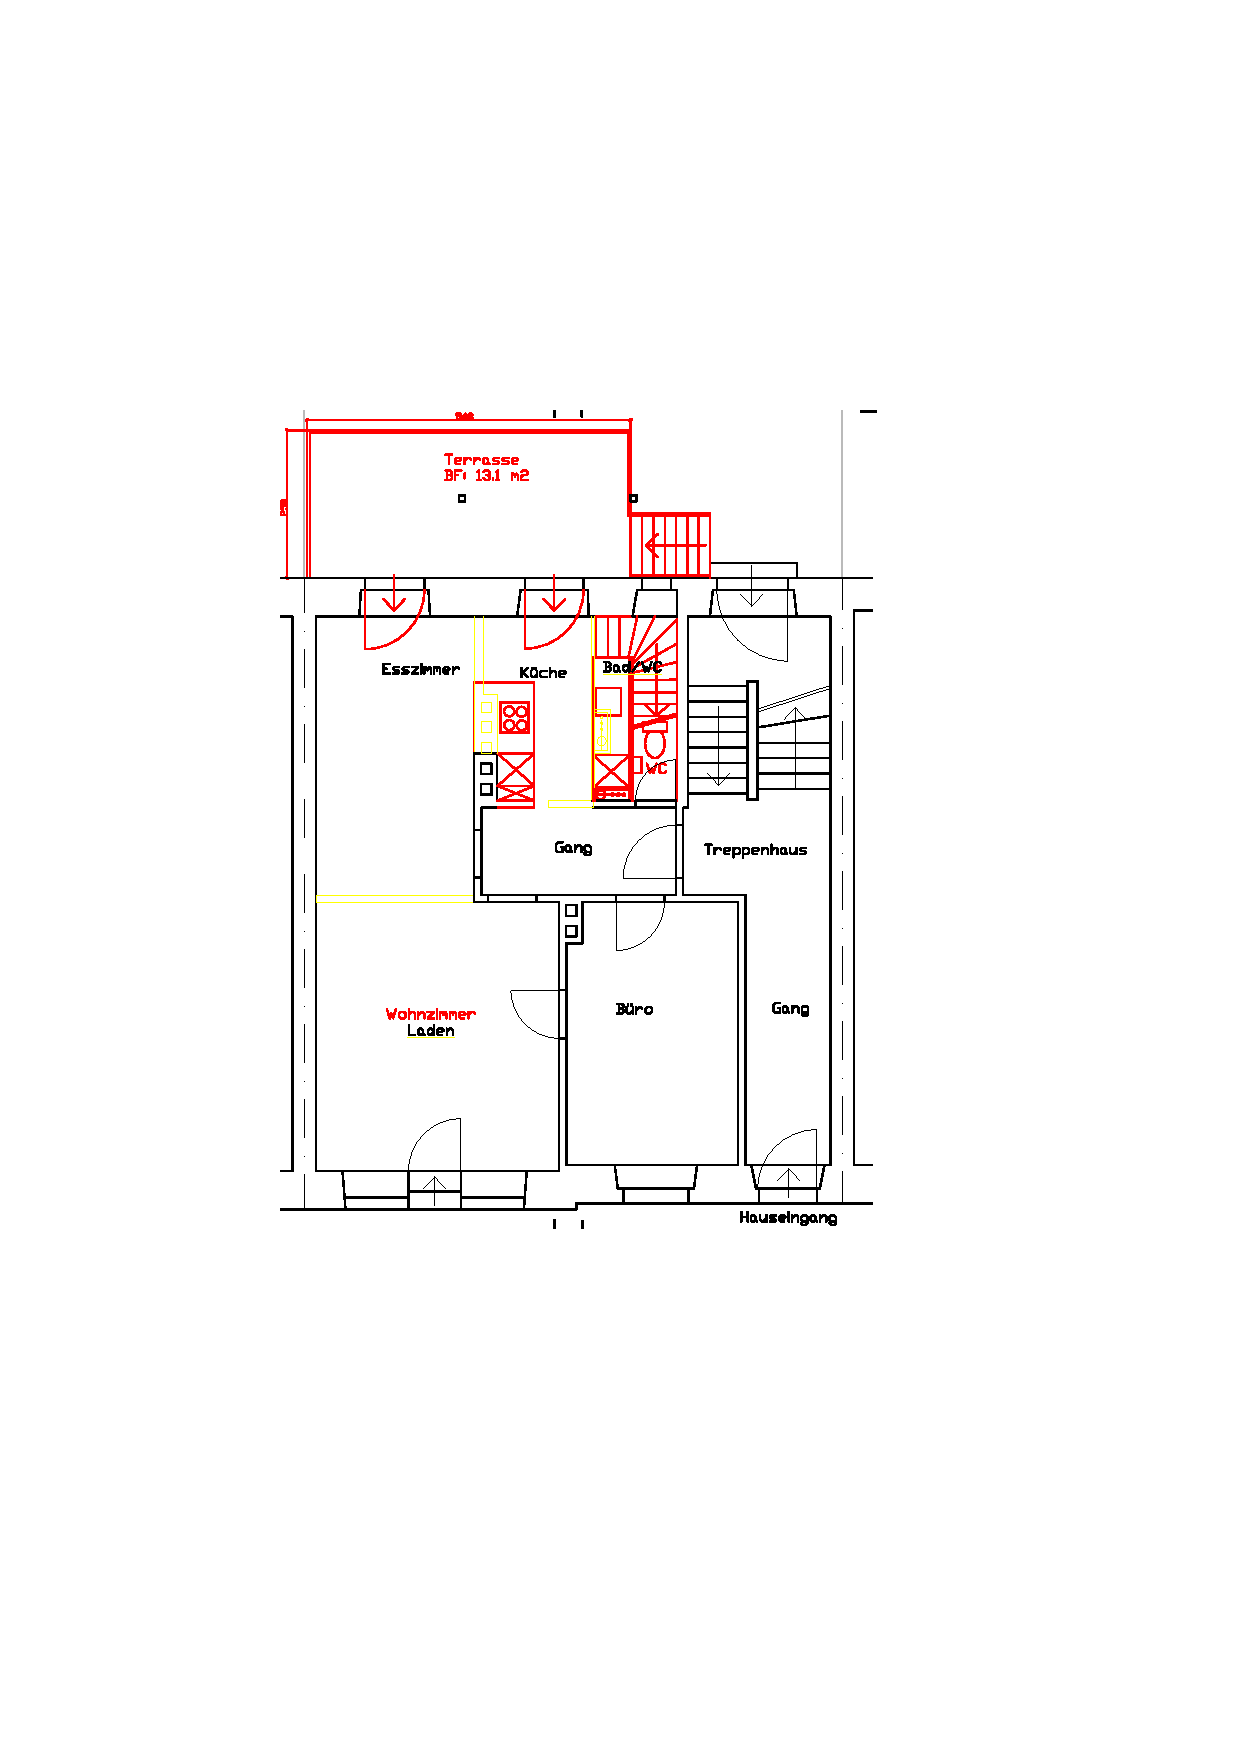
\includegraphics[scale=1.2]{Hongg_EG_Plan.pdf}
		\caption{Floor plan of residential building (Hongger) ground - 1$^{st}$ floor}
		\label{fig:hongg_eg_plan}
		\end{figure}
		
		\begin{figure}[htbp]
		\centering
		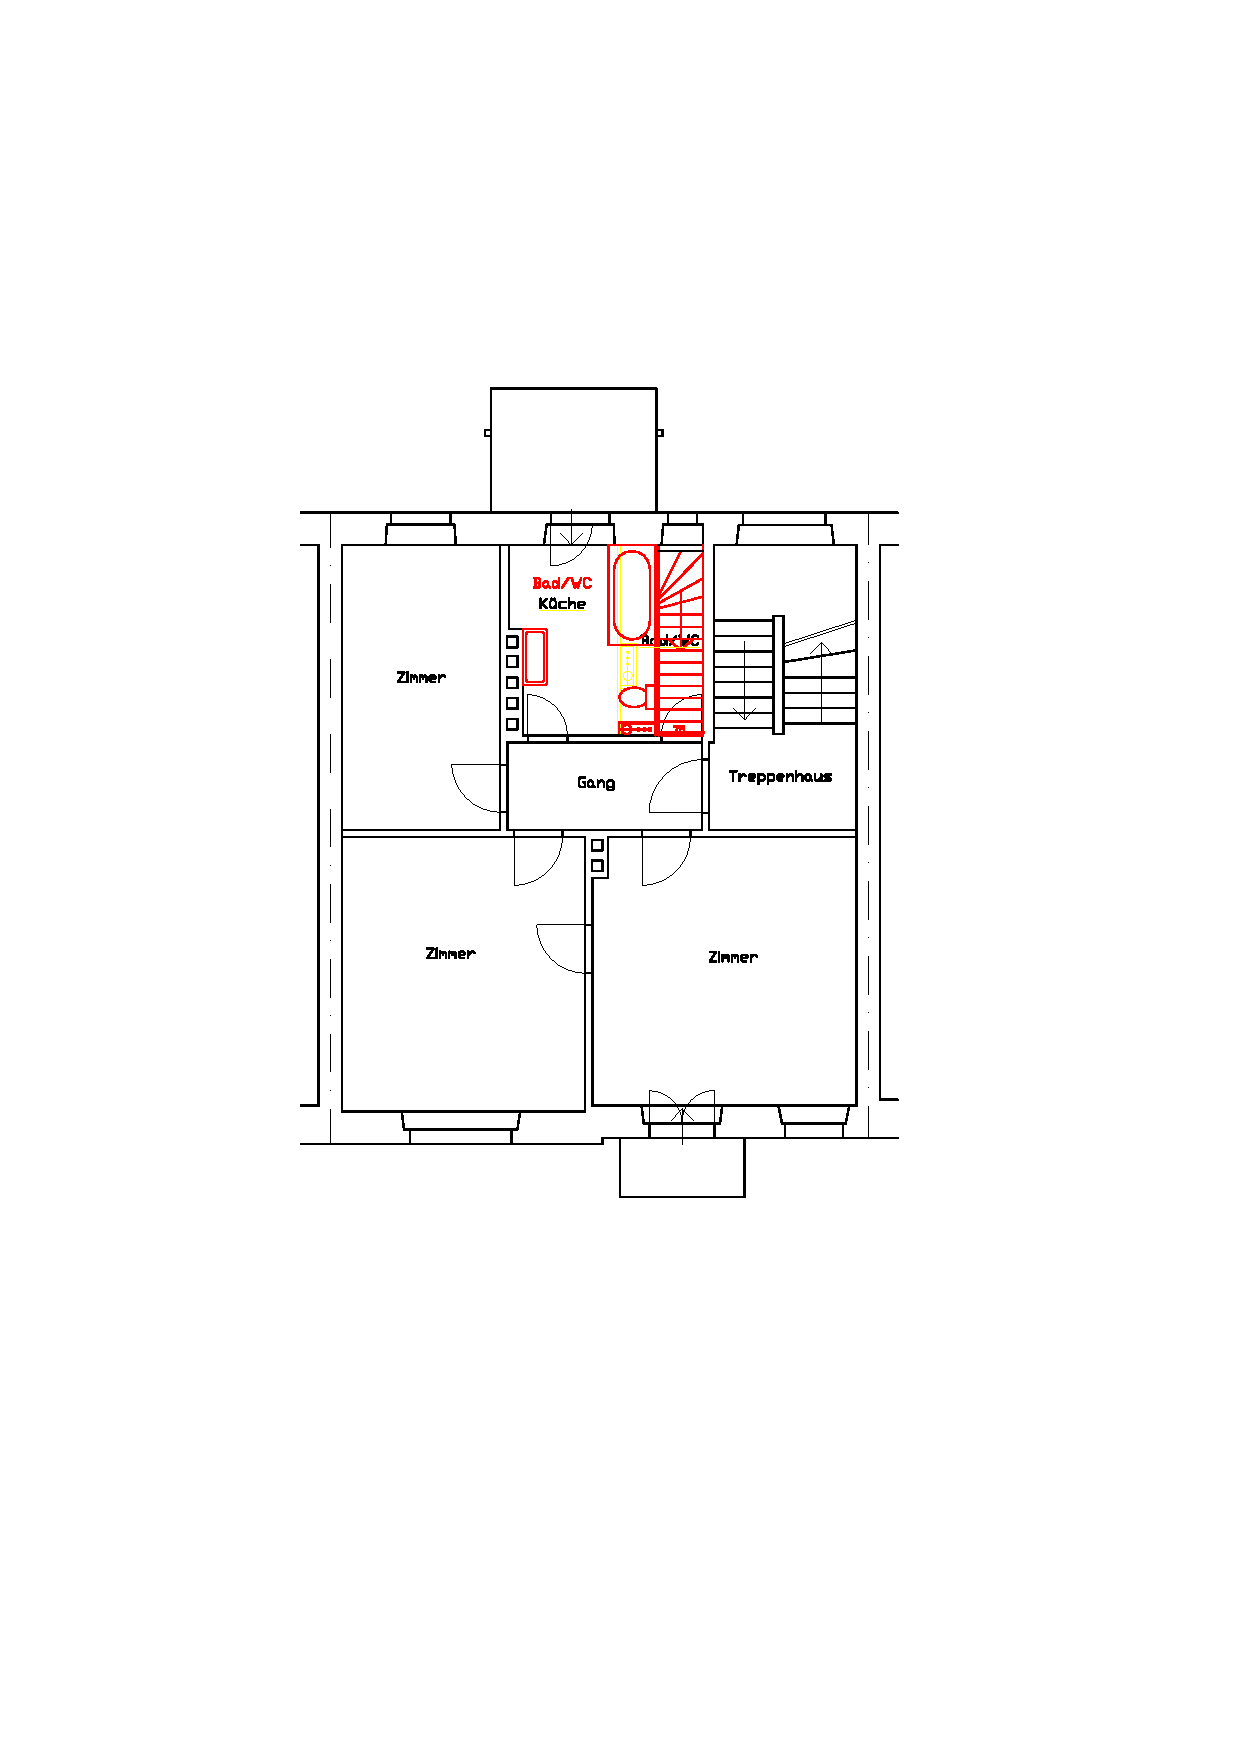
\includegraphics[scale=1.2]{Hongg_1OG_Plan.pdf}
		\caption{Floor plan of residential building (Hongger) 1$^{st} - 4^{th}$ floor}
		\label{fig:hongg_og1_plan}
		\end{figure}


	\section{Building Model Construction}
		\textit{DesignBuilder} is used to model the building envelopes of both buildings. It is compatible with EnergyPlus and provides advanced tools to model building geometry and building energy systems. Firstly the geometry of buildings are created, and an EnergyPlus script was generated based on the created building geometry. Secondly, the occupant activities and schedules are defined in EnergyPlus. Finally, the model is ready for parameter variation analysis after a calibration process under an un-heated period.

		\subsection{Building Geometry}
			The actual geometry of the building is not specifically given in the report provided by \textit{Lemon Consult} \cite{SIAPreviousreport}, where both buildings' floor plannings and building envelop specifications are provided. However, a detailed floor plan and some geometries are given in pdf format as shown in Figure \ref{fig:sumatra_og2}, and \ref{fig:sumatra_og3}, \ref{fig:hongg_eg_plan}, \ref{fig:hongg_og1_plan}. Therefore, in order to obtain an accurate building geometry, the pdf floor plan is firstly scaled to fit its nominated geometry, then a drawing file with correct scales are made according to the given pdf floor plans. After the drawing files are completed, they can be imported to DesignBuilder as a construction basis as shown in Figure \ref{fig:SumatraDxf} and \ref{fig:HonggerDxf}.

			\begin{figure}[H]
			\centering
			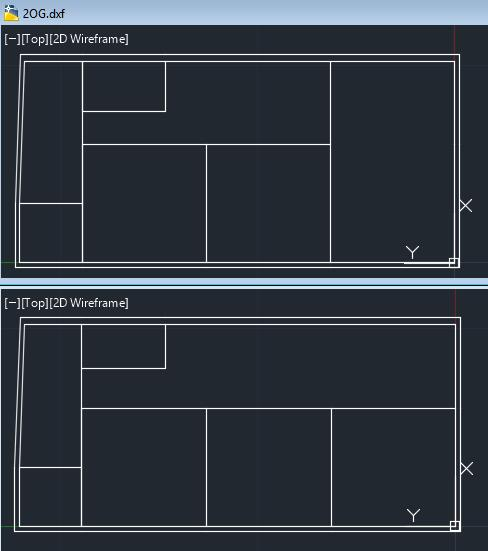
\includegraphics[scale=0.8]{Sumatra_dxf.jpg}
			\caption{dxf drawing files for office building}
			\label{fig:SumatraDxf}
			\end{figure}
			
			\begin{figure}[H]
			\centering
			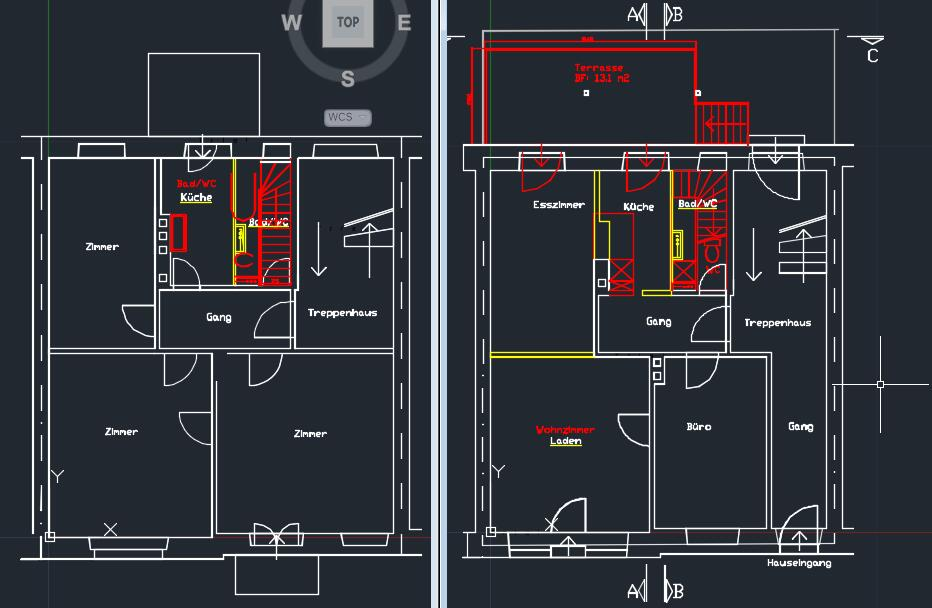
\includegraphics[scale=0.55]{Hongger_dxf.jpg}
			\caption{dxf drawing files for residential building}
			\label{fig:HonggerDxf}
			\end{figure}
			

			After the outline of buildings are constructed, windows and doors are defined. The window and door geometries of the office building and the residential building are shown in the Table \ref{table:HonggerWindowLayout} and Table \ref{table:SumatraWindowLayout}. The window code specify the size and thermal property of a type of window, and the detailed window code information can be found in Table \ref{tab:SumatraWindow}. \\

				%\newpage
				\begin{table}[H]
				\centering
				\caption{Window Layout of Residential Building}
				\begin{tabular}{  c | c | c | c  }
					\hline
					\multicolumn{4}{c}{Ground Floor} \\ 
					\hline
					Orientation & Location & Code & Number of window \\ \hline
					\multirow{4}{*}{SW} & Terrasse & 2a & 2 \\ 
					 & WC & 3a & 1 \\ 
					 & Staircase & 1a & 1 \\ 
					 & Front Door & TH & 1 \\ \hline
					\multirow{3}{*}{NE} & Laden & 1a & 1 \\ 
					 & Office & 4a & 1 \\ 
					 & Door & TH 1a & 1 \\ \hline
					\multicolumn{4}{c}{1st Floor to 4th Floor}\\ \hline
					\multirow{4}{*}{SW} & Terrasse & 2a & 1 \\ 
					 & WC & 3a & 1 \\ 
					 & Office & 4a & 1 \\ 
					 & Corridor & TH 1a & 1 \\ \hline
					\multirow{2}{*}{NE} & Office & 4a & 2 \\ 
					 & Terrasse & 2a & 1 \\ 
					 \hline
				\end{tabular}
				\label{table:HonggerWindowLayout}
				\end{table}


				\begin{table}[H]
				\centering
				\caption{Window Layout of Office Building}
				\begin{tabular}{  c | c | c | c  }
					\hline
					\multicolumn{4}{c}{Ground Floor}\\
					\hline
					Orientation & Location & Code & Number of windows\\ \hline
					\multirow{4}{*}{W} & Right Office & FE1 & 2 \\
					 & Conference room & FE1 & 2 \\
					 & Large office & FE1 & 2 \\
					 & Corridor & FE6 & 2 \\ \hline
					S & Large office & FE6 & 2 \\ \hline
					\multicolumn{4}{c}{1st Floor and 2nd Floor}\\\hline
					\multirow{4}{*}{W} & Right Office & FE1 & 2 \\ 
					 & Conference room & FE1 & 2 \\ 
					 & Large office & FE1 & 2 \\ 
					 & small office & FE1 & 1 \\ \hline
					S & Large office & FE1 & 1 \\ \hline
					\multicolumn{4}{c}{3rd Floor}\\ \hline
					\multirow{4}{*}{W} & Right Office & FE1 & 2 \\ 
					 & Middle office & FE1 & 2 \\ 
					 & Corner office & FE1 & 2 \\ 
					 & small office & FE1 & 1 \\ \hline
					\multirow{3}{*}{S} & Corner office & FE1 & 2 \\ 
					 & Kitchen and Corridor & FE4 & 1 \\ 
					 & Kitchen and Corridor & FE5 & 1 \\ \hline
					\multirow{2}{*}{E} & Kitchen and Corridor & FE7 & 1 \\ 
					 & Staircase & FE3 & 1 \\ \hline
				\end{tabular}
				\label{table:SumatraWindowLayout}
				\end{table}


			
				\begin{table}[H]
				\centering
				\caption{Office building window specification}
			    \begin{tabular}{ccccc}
			    	\toprule
				    \multicolumn{1}{p{3em}}{Code} & \multicolumn{1}{p{3.785em}}{U-Value W/m$^2$K} & \multicolumn{1}{c}{Number of window} & \multicolumn{1}{p{4.215em}}{Unit area \newline{} m$^2$} & \multicolumn{1}{p{5em}}{Total area \newline{} m$^2$} \\
				    \midrule
				    \multicolumn{1}{c}{FE1} & 2.001 & 33   & 6    & 198 \\
				    \midrule
				    \multicolumn{1}{c}{FE2} & 2.500 & 1    & 8.125 & 8.13 \\
				    \midrule
				    \multicolumn{1}{c}{FE3} & 2.500 & 1    & 2.7  & 2.7 \\
				    \midrule
				    FE4  & 2.048 & 3    & 3.5  & 10.5 \\
				    \midrule
				    FE5  & 2.072 & 3    & 2.598 & 7.79 \\
				    \midrule
				    FE6  & 2.028 & 2    & 2.25 & 4.5 \\
				    \midrule
				    FE7  & 2.042 & 2    & 2.88 & 5.76 \\
				    \midrule
				    FE8  & 1.907 & 3    & 0.975 & 2.93 \\
				    \bottomrule
			    \end{tabular}%
				\label{tab:SumatraWindow}%
				\end{table}%

				% Table generated by Excel2LaTeX from sheet 'HonggerWindows'
				\begin{table}[H]
				\centering
				\caption{Residential building window specification}
				    \begin{tabular}{ccccc}
				    \toprule
				     \multicolumn{1}{p{3em}}{Code} & \multicolumn{1}{p{3.785em}}{U-Value W/m$^2$K} & \multicolumn{1}{c}{Number of window} & \multicolumn{1}{p{4.215em}}{Unit area \newline{} m$^2$} & \multicolumn{1}{p{5em}}{Total area \newline{} m$^2$} \\
				    \midrule
				    FE-EG-1a & 2.379 & 1    & 6.9  & 9.9 \\
				    \midrule
				    FE-EG-2a & 2.388 & 10   & 2.6  & 26 \\
				    \midrule
				    FE-EG-3a & 2.19 & 5    & 0.6  & 3 \\
				    \midrule
				    FE-EG-4a & 2.285 & 13   & 1.6  & 20.8 \\
				    \midrule
				    FE-TH-1a & 2.33 & 1    & 2.88 & 3.7 \\
				    \midrule
				    Tür-TH & 3.5  & 1    & 2.5  & 2.5 \\
				    \bottomrule
				    \end{tabular}%
				\label{tab:HonggWindow}%
				\end{table}%
		

		\subsection{Building Envelope Constructions}
			After the building geometry is constructed, the building wall and window elements are assigned a set of thermal properties based on measurememts.
			Both buildings are uninsulated reinforced concrete structure buildings with thin outer and inner plaster layers. The detailed building wall of both buildings as well as their thermodynamic properties are measured from the actural building and are shown in Table \ref{tab:SumatraWallMaterial} and Table \ref{tab:HonggerWallMat}. The window properties and geometries of both buildings can be found in Table \ref{tab:SumatraWindow} and Table \ref{tab:HonggWindow}. After the building material are assigned to all part of the buildings, static calculation and dynamic calculation can be performed. Figure \ref{fig:SumatraDB} and \ref{fig:HonggDB} shows a completed office and residential building DesignBuilder model with geometry and material information.\\
			
			\newpage
			\begin{table}[h!]
			  \centering
			\caption{Wall material list of office building}
			    \begin{tabular}{lrrrcrr}
			    \toprule
			         & \multicolumn{1}{p{4em}}{Thickness \newline{}(m)} & \multicolumn{1}{p{3.145em}}{Density \newline{}(kg/m$^3$)} & \multicolumn{1}{p{3.285em}}{Lambda \newline{}(W/mK)} & \multicolumn{1}{p{5.1em}}{Heat \newline{}Capacity (kJ/kg.K)} & \multicolumn{1}{p{3.5em}}{R Value \newline{}(m$^2$K/W)} & \multicolumn{1}{p{3.145em}}{U Value \newline{}(W/m$^2$K)} \\
			    \midrule
			    \multicolumn{7}{p{26.86em}}{EG East Wall} \\
			    \multicolumn{1}{l}{Outside convection coefficient} &      &      &      &      &      &  \\
			    \multicolumn{1}{p{6.785em}}{Outer Layer} & 0.36 & 2400 & 2.5  & 1    & 0.144 &  \\
			    \multicolumn{1}{p{6.785em}}{Inner Layer} & 0.01 & 1400 & 0.7  & 1    & 0.014 &  \\
			    \multicolumn{3}{p{13.93em}}{Inside convection coefficientr} &      &      & 0.13 & 7.7 \\
			         &      &      &      &      & 0.288 & 3.4703 \\
			    \midrule
			    \multicolumn{7}{p{26.86em}}{West and Other Wall} \\
			    \multicolumn{4}{p{17.215em}}{Outside convection Coefficient} &      & 0.04 & 25 \\
			    \multicolumn{1}{p{6.785em}}{Outside Layer} & 0.02 & 1400 & 0.7  & 1    & 0.029 & 35 \\
			    \multicolumn{1}{p{6.785em}}{Layer2} & 0.05 & 1100 & 0.44 & 0.94 & 0.114 & 8.8 \\
			    \multicolumn{1}{p{6.785em}}{Middle Layer} & 0.02 & 120  & 0.056 & 1.56 & 0.357 & 2.8 \\
			    \multicolumn{1}{p{6.785em}}{Inside Layer} & 0.15 & 2400 & 2.5  & 1    & 0.06 & 16.667 \\
			    \multicolumn{4}{p{17.215em}}{Inside Convection Coefficient} &      & 0.13 & 7.7 \\
			         &      &      &      &      & 0.729 & 1.3713 \\
			    \midrule
			    \multicolumn{7}{p{26.86em}}{East Wall (Thick)} \\
			    \multicolumn{3}{p{13.93em}}{Outside convection Coefficient} &      &      & 0.04 & 25 \\
			    \multicolumn{1}{p{6.785em}}{Outside Layer} & 0.02 & 1800 & 0.87 & 1    & 0.023 & 43.5 \\
			    \multicolumn{1}{p{6.785em}}{Middle Layer} & 0.36 & 1100 & 0.44 & 0.94 & 0.818 & 1.2222 \\
			    \multicolumn{1}{p{6.785em}}{Inside Layer} & 0.02 & 1400 & 0.7  & 1    & 0.029 & 35 \\
			    \multicolumn{3}{p{13.93em}}{Inside Convection Coefficient} &      &      & 0.13 & 7.7 \\
			         &      &      &      &      & 1.04 & 0.9619 \\
			    \midrule
			    \multicolumn{7}{p{26.86em}}{Ceiling} \\
			    \multicolumn{3}{p{13.93em}}{Outside convection coefficient} &      &      & 0.04 & 25 \\
			    \multicolumn{1}{p{6.785em}}{Layer 1} & 0.04 & 120  & 0.056 & 1.56 & 0.714 &  \\
			    \multicolumn{1}{p{6.785em}}{Layer 2} & 0.0042 & 1100 & 0.23 & 1    & 0.15 &  \\
			    \multicolumn{1}{p{6.785em}}{Layer 3} & 0.0035 & 1100 & 0.23 & 1    & 0.015 &  \\
			    \multicolumn{1}{p{6.785em}}{Layer 4} & 0.001 & 980  & 0.5  & 1.8  & 0.002 &  \\
			    \multicolumn{1}{p{6.785em}}{Layer 5} & 0.22 & 2400 & 2.5  & 1    & 0.088 &  \\
			    \multicolumn{3}{p{13.93em}}{Inside convection coefficientr} &      &      & 0.13 & 7.7 \\
			         &      &      &      &      & 1.139 & 0.8777 \\
			    \midrule
			    \multicolumn{7}{p{26.86em}}{Ground} \\
			    \multicolumn{3}{p{13.93em}}{Outside convection coefficient} &      &      & 0.13 & 7.7 \\
			    \multicolumn{1}{p{6.785em}}{Layer 1} & 0.01 & 120  & 0.056 & 1.56 & 0.179 &  \\
			    \multicolumn{1}{p{6.785em}}{Layer 2} & 0.22 & 2400 & 2.5  & 1    & 0.088 &  \\
			    \multicolumn{3}{p{13.93em}}{Inside convection coefficientr} &      &      & 0.13 & 7.7 \\
			         &      &      &      &      & 0.526 & 1.9 \\
			    \bottomrule
			    \end{tabular}%
			  \label{tab:SumatraWallMaterial}%
			\end{table}%

			\newpage
			\begin{table}[h!]
			  \centering
			\caption{Residential building wall material}
			    \begin{tabular}{rrrrcrr}
			    \toprule
			         & \multicolumn{1}{p{3.93em}}{Thickness (m)} & \multicolumn{1}{p{3.07em}}{Density (kg/m$^3$)} & \multicolumn{1}{p{3.145em}}{Lambda (W/mK)} & \multicolumn{1}{p{5.em}}{Heat \newline{}Capacity (kJ/kg.K)} & \multicolumn{1}{p{3.55em}}{R Value (m$^2$K/W)} & \multicolumn{1}{p{3.55em}}{U Value (W/m$^2$K)} \\
			    \midrule
			    \multicolumn{7}{c}{External Wall} \\
			    \midrule
			    \multicolumn{1}{l}{Outside convection Coefficient} &      &      &      &      & 0.04 & 25 \\
			    \multicolumn{1}{l}{Outside Layer} & 0.04 & 1800 & 0.87 & 1    & 0.046 & 21.75 \\
			    \multicolumn{1}{l}{Middle Layer} & 0.6  & 1800 & 0.8  & 0.94 & 0.75 & 1.3333 \\
			    \multicolumn{1}{l}{Inside Layer} & 0.02 & 1400 & 0.7  & 1    & 0.0286 & 35 \\
			    \multicolumn{1}{l}{Inside Convection Coefficient} &      &      &      &      & 0.1299 & 7.7 \\
			         &      &      &      &      & 0.9944 & 1.0056 \\
			    \midrule
			    \multicolumn{7}{c}{Ground} \\
			    \midrule
			    \multicolumn{1}{l}{Outside convection coefficient} &      &      &      &      & 0.1299 & 7.7 \\
			    \multicolumn{1}{l}{Layer 1} & 0.02 & 900  & 0.25 & 1    & 0.08 &  \\
			    \multicolumn{1}{l}{Layer 2} & 0.1  &      &      &      & 0.15 &  \\
			    \multicolumn{1}{l}{Layer 3} & 0.03 & 1500 & 1.5  & 2.1  & 0.02 &  \\
			    \multicolumn{1}{l}{Layer 4} & 0.03 & 500  & 0.13 & 1.6  & 0.2308 &  \\
			    \multicolumn{1}{l}{Inside convection coefficientr} &      &      &      &      & 0.1299 & 7.7 \\
			         &      &      &      &      & 0.7405 & 1.3504 \\
			    \midrule
			    \multicolumn{7}{c}{Ceiling} \\
			    \midrule
			    \multicolumn{1}{l}{Outside convection coefficient} &      &      &      &      & 0.1299 & 7.7 \\
			    \multicolumn{1}{l}{Layer 1} & 0.02 & 1400 & 0.7  & 1    & 0.0286 &  \\
			    \multicolumn{1}{l}{Layer 2} & 0.2  & 2300 & 2.3  & 1    & 0.087 &  \\
			    \multicolumn{1}{l}{Layer 3} & 0.02 & 1500 & 1.5  & 2.1  & 0.0133 &  \\
			    \multicolumn{1}{l}{Layer 4} & 0.03 & 500  & 0.13 & 1.6  & 0.2308 &  \\
			    \multicolumn{1}{l}{Inside convection coefficientr} &      &      &      &      & 0.1299 & 7.7 \\
			         &      &      &      &      & 0.6194 & 1.6145 \\
			    \bottomrule
			    \end{tabular}%
			  \label{tab:HonggerWallMat}%
			\end{table}%



			%\newpage
			\begin{figure}[H]
			\centering
			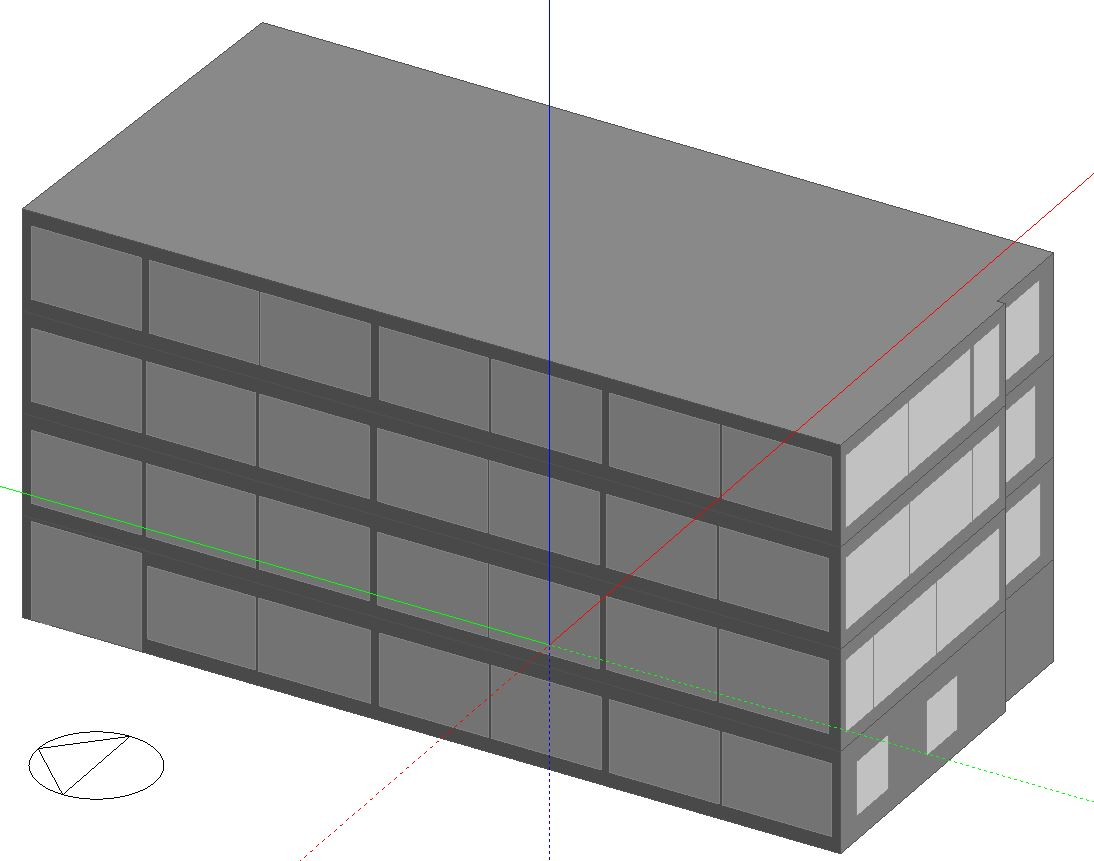
\includegraphics[scale=0.4]{SumatraDesignBuilderModel.JPG}
			\caption{Office building DesignBuilder model}
			\label{fig:SumatraDB}
			\end{figure}

			\begin{figure}[H]
			\centering
			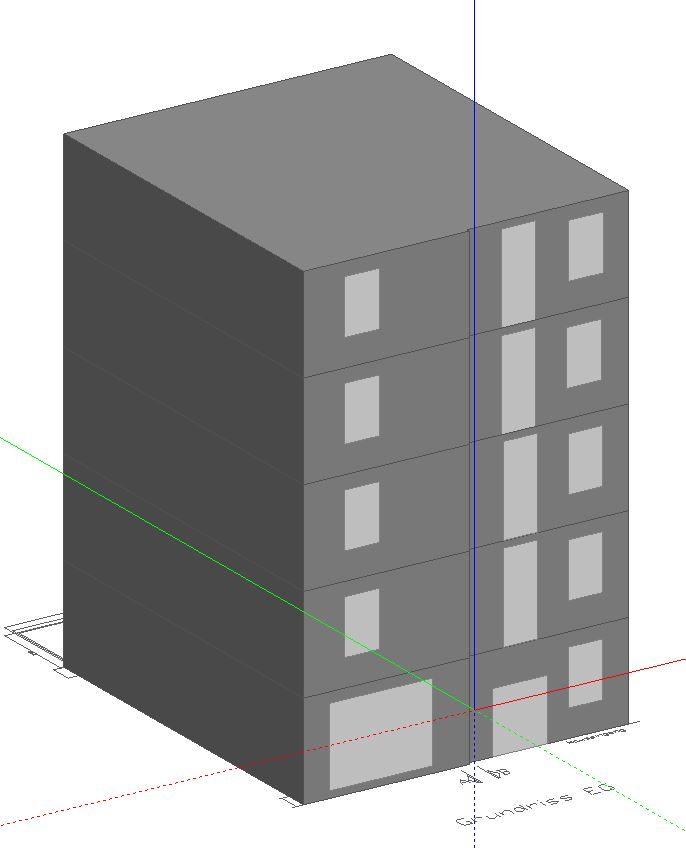
\includegraphics[scale=0.4]{HonggDesignBuilderModel.JPG}
			\caption{Residential building DesignBuilder model}
			\label{fig:HonggDB}
			\end{figure}


	\section{Selection of Simulation Tools}
		Crawley and Hand et.al provided a comprehensive review on currently in-use building energy simulation tools back in 2008, and it include a brief review of EnergyPlus 1.2.2 and its basis building simulation tools \cite{crawley2008contrasting}. As EnergyPlus is compatible with building modeling software \textit{DesignBuilder}, it is more convenient to use it in this thesis comparing to other simulation tools. Additionally, as EnergyPlus is based on the features and capabilities of BLAST and DOE-2, these two tools are also briefly reviewed \cite{crawley2008contrasting}. However, the reviewed EnergyPlus version is more than 10 years old, it is believed that most of the functions have been updated and improved since then. \\

		\textbf{Building BLAST}\\
			The BLAST system predicts building energy consumption, building energy system performance and building costs \cite{crawley2008contrasting}. It contains three major subprograms: Space Loads Prediction, Air System Simulation, and Central Plant. \textit{Space Loads Prediction} computes hourly space loads based on the given hourly weather data, building construction properties and operation details. It uses a radiant, convective, and conductive heat balance for all surfaces and a heat balance of indoor air \cite{crawley2008contrasting}. The energy balance equations include heat transmission, solar loads, internal heat gains, air infiltration loads, and temperature control strategy used to manipulate the indoor temperature. BLAST can be used on new or existing buildings of almost any type and shape \cite{crawley2008contrasting}.\\

		\textbf{DOE-2.1E}\\
			DOE-2 predicts hourly energy consumption and energy cost for a building based on the given weather information, building geometry, HVAC description, and utility cost. DOE-2 has one subprogram to translate input (BDL Processor), and four simulation subprograms namely \textit{Loads, Systems, Plant, and ECON (Economics)}.\\
			\textit{Loads, Systems and Plant} are executed in sequence, with the output of the predecessor become the input of the next program in sequence. The output then becomes the input to \textit{Economics} \cite{crawley2008contrasting}. Each of the simulation subprograms can also generate printable reports of the results of its calculations.\\
			DOE-2 has been used extensively for more than 35 years for both building design studeis, retrofit analysis, and for developing and testing building energy standards \cite{crawley2008contrasting}.\\
		

		\textbf{EnergyPlus}\\
			\textit{EnergyPlus} is a modular and structured code based calculation engine. As mentioned above, it is based on the most popular features and functions of BLAST and DOE-2 and it is a more advanced tool compared to the previous two simulation engines. It is a simulation engine with input and output as text files. Loads are firstly calculated at a user-defined time step, then passed on to the building systems simulation module at the same time step \cite{crawley2008contrasting}. The EnergyPlus building system simulation module calculates heating and cooling system and plant and electrical system response. The integrated simulation also capable to evaluate realistic system controls, moisture adsorption and deorption in building elements, radiant heating and cooling system and interzone air flow \cite{crawley2008contrasting}.\\



	\section{SIA Norms}
		Most of the building occupancy and activity assumptions are from the standard values published by the Swiss society of engineers and architects (hereinafter: SIA). The SIA standards range from energy consumption calculation formulars to the supporting informations about a particular building type or a room type. They also include a reference standard weather data set for most of the cities in Switzerland. Here are the main SIA standards that are used or taken into account in this thesis which are discussed:\\

		\textbf{SIA 380/1: Thermal energy in buildings}\\
		This SIA 380/1 standard was published in 2009 replacing its predecessor SIA 380/1 (2007). It is often used with other standardized calculation parameters when assessing the energy efficiency of existing buildings \cite{SIAPreviousreport}. It also serves as a forecasting tool to evaluate the refurbishment plans. However, the building usually consume less energy than what the calculation suggest, and this issue become more severe as the building envelope gets worse as shown in Figure \ref{fig:SIA380PG}. When using SIA 380/1 to calculate the entitlements for governmental energy certificates, standardized data is used, while when using SIA 380/1 for energy consulting, design and optimizations, the best known data can be used \cite{SIAPreviousreport}.\\


		\textbf{SIA 2028: Weather Data}\\
		SIA also published a set of standard weather information for most cities in Switzerland. It splits Switzerland into several climate zones and each zone would have their specific climate patten and typical weather data for energy calculation. As SIA 380/1 uses monthly average temperature and monthly heating degree days to calculate annual heating demand, this SIA standard weather data is used in this thesis as a reference guide.\\

		The weather data set includes monthly and annual average temperature, monthly and annual heating degree days, monthly and annual solar radiation in north, south, east, west and horizontal surfaces. In addition, SIA also published another set of standard hourly data on its partner website \textit{www.energytool.ch} for purchase.\\

		\textbf{SIA 2024: Room utilization data for energy calculations}\\
		Apart from the standard calculation of SIA 380/1 which uses monthly and annual unit area standard values for a specific building type, SIA also developed a dynamic building energy analysis approach SIA382/1 which use hourly unit area data for a specific room or zone type. SIA 2024 is the unification of assumptions about occupancy and equipment or appliance usage level for specific zone types such as corridor, bedroom, living room and toilet.\\

		The assumptions listed in SIA 2024 include room heating and cooling setpoints, maximum supply wind speed, typical room area, window-to-wall ratio, window g-values, room occupancy level and activity level, internal gain level, electricity usage level and activities, minimum and typical amount of outdoor air and ventilation level, lighting and domestic hot water demand etc.\\

		These assumptions are used in calculations and verifications according to energy and building service standard. For occupancy and appliance level assumptions, it gives not only a specific value but also a resonable range which enable a stochastic building energy consumption analysis. SIA 2024 has provide assumptions for 46 different zone types, which cover a majority of building types \cite{SIA2024Shop}.

		\section{Weather Data}
		A number of data files or weather data are used in this research. These weather files and data include: (1) a typical SIA standard monthly weather and hourly weather; (2) a typical meteorological year (TMY) weather file obtained from \textit{Meteonorm} which contains an average or typical weather information from the recent 10 to 15 years; (3) a created data file based on weather station measurement in 2015; (4) a created heat island weather file. These weather data can be grouped into two categories according to their functions.

		\subsection{Weather Data For Static Calculation}
		\textbf{SIA 381/2 Weather Data}\\
		SIA has published a standard weather data set \textit{SIA 381/2 Klimadaten zi Emfehlung SIA 380/1} (Recommended climate data for SIA 380/1) in 1988. It splits Switzerland into a number of climate zones. It also contain monthly weather data set for most main cities in Switzerland. The useful information from this weather dataset are monthly air temperature, monthly heating days, monthly heating degree days and monthly solar radiation on different orientation surfaces.\\


		\begin{table}[H]
		  \centering
		  \small
		\caption{SIA 381/2 Weather Data in Zurich}
		    \begin{tabular}{|p{4.5em}|c|c|c|c|c|c|c|c|c|c|c|c|c|}
		    \toprule
		    \multicolumn{14}{|c|}{SIA 381/2 Weather Data} \\
		    \midrule
		    \textbf{Month} & \textbf{Jan} & \textbf{Feb} & \textbf{Mar} & \textbf{Apr} & \textbf{May} & \textbf{Jun} & \textbf{Jul} & \textbf{Aug} & \textbf{Sep} & \textbf{Oct} & \textbf{Nov} & \textbf{Dec} & \textbf{Sum} \\
		    \midrule
		    Average Temperature ($^o$C) & 0.1  & 2.1  & 4.8  & 9    & 14   & 18   & 19   & 18   & 16   & 11   & 5.4  & 0.6  & 3260 \\
		    \midrule
		    HDD  & 615  & 501  & 467  & 255  & 110  & 23   & 7    & 6    & 35   & 207  & 433  & 601  & 1091 \\
		    \midrule
		    Solar Energy at N (MJ/m$^2$) & 33   & 48   & 78   & 108  & 158  & 172  & 168  & 116  & 89   & 61   & 32   & 28   & 2248 \\
		    \midrule
		    Solar Energy at E (MJ/m$^2$) & 57   & 96   & 170  & 243  & 299  & 320  & 330  & 284  & 212  & 127  & 61   & 49   & 3133 \\
		    \midrule
		    Solar Energy at S (MJ/m$^2$) & 149  & 217  & 281  & 315  & 299  & 290  & 318  & 337  & 347  & 272  & 166  & 142  & 2303 \\
		    \midrule
		    Solar Energy at W (MJ/m$^2$) & 67   & 110  & 170  & 248  & 294  & 308  & 330  & 284  & 227  & 138  & 70   & 57   & 4156 \\
		    \midrule
		    Horizontal Solar Energy (MJ/m$^2$)& 94   & 166  & 299  & 450  & 565  & 616  & 648  & 526  & 385  & 227  & 104  & 76   & 1564 \\
		    \midrule
		    Solar Energy at NE (MJ/m$^2$)& 43   & 68   & 115  & 162  & 217  & 235  & 235  & 182  & 137  & 88   & 44   & 37   & 2653 \\
		    \midrule
		    Solar Energy at SW (MJ/m$^2$)& 100  & 154  & 219  & 279  & 296  & 299  & 324  & 309  & 281  & 194  & 108  & 90   & 2653 \\
		    \bottomrule
		    \end{tabular}%
		  \label{tab:WeatherSIA3812}%
		\end{table}%



			\textbf{2015 Weather Data}\\
				The 2015 Zurich weather data for static calculation is based on the information from the given 2015 .\textit{epw} weather file. The hourly data is firstly extracted from the weather file then calculate the monthly average. \textit{Rhino6} and \textit{Grasshopper} are also used to extract the hourly data as well as calculating the average monthly solar radiation on the nominal orientations (N, E, S, W, NE, SW, and Horizontal). The resultant monthly weather data is shown at Table \ref{tab:2015Monthly}. Table \ref{tab:StaticWeatherCompare} below shows a comparison of two different weather data.
				
				\begin{table}[H]
				  \centering
				  \small
				\caption{2015 Zurich Monthly Data}
				    \begin{tabular}{|p{5.3em}|r|r|r|r|r|r|r|r|r|r|r|r|r|}
				    \toprule
				    \multicolumn{14}{|c|}{2015 Weather Data} \\
				    \midrule
				    \textbf{Month} & \multicolumn{1}{l|}{\textbf{Jan}} & \multicolumn{1}{l|}{\textbf{Feb}} & \multicolumn{1}{l|}{\textbf{Mar}} & \multicolumn{1}{l|}{\textbf{Apr}} & \multicolumn{1}{l|}{\textbf{May}} & \multicolumn{1}{l|}{\textbf{Jun}} & \multicolumn{1}{l|}{\textbf{Jul}} & \multicolumn{1}{l|}{\textbf{Aug}} & \multicolumn{1}{l|}{\textbf{Sep}} & \multicolumn{1}{l|}{\textbf{Oct}} & \multicolumn{1}{l|}{\textbf{Nov}} & \multicolumn{1}{l|}{\textbf{Dec}} & \multicolumn{1}{l|}{\textbf{Sum}} \\
				    \midrule
				    Average Temperature ($^o$C) & 3.7  & 1.5  & 8.2  & 12   & 16   & 20   & 25   & 23   & 15   & 11   & 9    & 5.1  &  \\
				    \midrule
				    Heating Degree Days & 498  & 519  & 344  & 149  & 31   & 0    & 0    & 0    & 18   & 225  & 268  & 462  & 2513.1 \\
				    \midrule
				    Solar Energy at N (MJ/m$^2$) & 25   & 42   & 62   & 86   & 116  & 158  & 150  & 107  & 74   & 46   & 30   & 23   & 919.15 \\
				    \midrule
				    Solar Energy at E (MJ/m$^2$) & 55   & 103  & 176  & 238  & 289  & 301  & 332  & 278  & 185  & 113  & 65   & 41   & 2176.1 \\
				    \midrule
				    Solar Energy at S (MJ/m$^2$) & 183  & 213  & 304  & 298  & 244  & 237  & 245  & 284  & 279  & 238  & 146  & 116  & 2786.3 \\
				    \midrule
				    Solar Energy at W (MJ/m$^2$) & 67   & 97   & 186  & 233  & 261  & 294  & 299  & 258  & 206  & 127  & 61   & 52   & 2140.7 \\
				    \midrule
				    Horizontal Solar Energy (MJ/m$^2$)& 104  & 174  & 316  & 446  & 549  & 596  & 605  & 512  & 353  & 208  & 108  & 78   & 4049.9 \\
				    \midrule
				    Solar Energy at NE (MJ/m$^2$)& 26   & 51   & 92   & 140  & 202  & 231  & 244  & 179  & 108  & 58   & 33   & 24   & 1388.6 \\
				    \midrule
				    Solar Energy at SW (MJ/m$^2$)& 146  & 167  & 269  & 287  & 273  & 282  & 288  & 290  & 268  & 204  & 112  & 97   & 2683.8 \\
				    \bottomrule
				    \end{tabular}%
				  \label{tab:2015Monthly}%
				\end{table}%

				% Table generated by Excel2LaTeX from sheet 'Sheet2'
				\begin{table}[htbp]
				  \centering
				\caption{Weather Data Comparison}
				    \begin{tabular}{|c|c|c|c|}
				    \toprule
				         & \multicolumn{1}{c}{SIA Standard Weather} & 2015 Weather & Typical Zurich Weather\\
				    \midrule
				    Heating Day & 208  & 175 & 213\\
				    \midrule
				    Heating Degree Day & 3260 & 2513 & 3283\\
				    \midrule
				    Annual Average Temperature & 8.5  & 12.3 & 9.75\\
				    \bottomrule
				    \end{tabular}%
				  \label{tab:StaticWeatherCompare}%
				\end{table}%


			\subsection{Weather Data For Dynamic Calculation}
				An .\textit{epw} weather file is needed for dynamic calculation using \textit{EnergyPlus}. The weather file is either from a meteological organization or from modifying an existing weather file. It contains a large number of weather information such as dry-bulb temperature, wet-bulb temperature, relative humidity, wind speed, wind direction, hourly solar radiation, cloudiness etc.\\

			\textbf{Typical Meteorological Year Weather File}\\
				A typical year Zurich weather file is obtained by using Meteonorm \cite{GeorgeThesis}. It is also the basis for other custom-made weather files that are used in this thesis such as 2015 station weather file and heat island weather file. The basic statistic information of the typical year weather file is shown at the 3$^{rd}$ column of Table \ref{tab:StaticWeatherCompare}. \\

			\textbf{2015 Weather File}\\
				The 2015 weather file is created from the typical Zurich weather file by replacing the dry bulb temperature, wet bulb temperature, relative humidity, wind speed, and wind direction by the actual hourly measured data in Zurich in 2015. The source of weather data is from \textit{Federal Office of Meteology and Climatology MeteoSwiss}. Considering the location of the two existing building, the weather station is chosen to be \textit{NABZUE}, which located at Zurich city as shown in Figure \ref{fig:NABZUE}. The exact location and the detailed weather file information is shown in Table \ref{tab:2015DataInformation}.

				\begin{figure}[H]
				\centering
				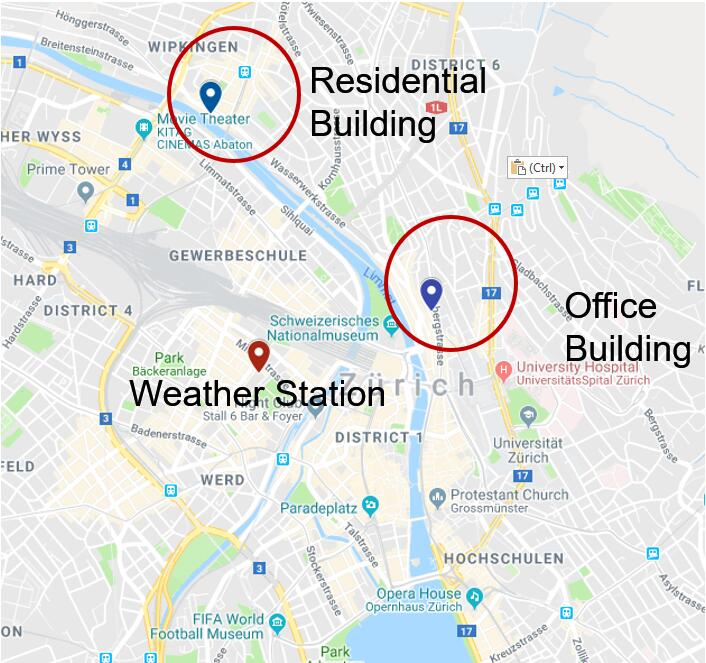
\includegraphics[scale=0.7]{WeatherStation.jpg}
				\caption{Weather Station Location}
				\label{fig:NABZUE}
				\end{figure}
				
				% Table generated by Excel2LaTeX from sheet 'Sheet2'
				\begin{table}[htbp]
				  \centering
				  \caption{Weather Data Information}
				    \begin{tabular}{|c|c|}
				    \toprule
				    \multicolumn{2}{|c|}{\textbf{2015 Weather Data Information}} \\
				    \midrule
				    Source & MeteoSwiss: IDAWEB \\
				    \midrule
				    Weather Station Code & NABZUE \\
				    \midrule
				    Station Coordinate & E 8$^o$31'49" , N 47$^o$22'39" \\
				    \midrule
				    Altitude & 409 m \\
				    \midrule
				    Year & 2015 \\
				    \bottomrule
				    \end{tabular}%
				  \label{tab:2015DataInformation}%
				\end{table}%



			\textbf{SIA382 Weather File}\\
				The full weather data is not fully accessible, and only the hourly temperature is obtained. However, the SIA 382 Weather File is only used to investigate the global warming effect in Zurich. The hourly stand weather temperature is used to replace the typical year weather temperature in the typical year weather file, while all other information remain the same as the 2015 weather data. The comparison between SIA 382 temperature and 2015 actual temperature \\ 

			\textbf{Urban Heat Island Weather File}\\
				Similarly, heat island weather is created based on measured data in year 2015 and aimed to investigate the heat island effect of Zurich city. Firstly, the temperature difference between building site temperature and the weather station data is recorded and average temperature difference is taken hour by hour as shown in Figure \ref{fig:HeatIslandConst} below. Then, based on the statistic results in Figure \ref{fig:HeatIslandConst}, a simple urban temperature variation rule as shown in Figure \ref{fig:HeatIslandRule} is applied on the 2015 weather temperature for each hour and create a new heat island weather temperature. Lastly, the new heat island temperature is imported to the .\textit{epw} weather file and become the \textit{heat island weather file}.


				\begin{figure}[H]
				\centering
				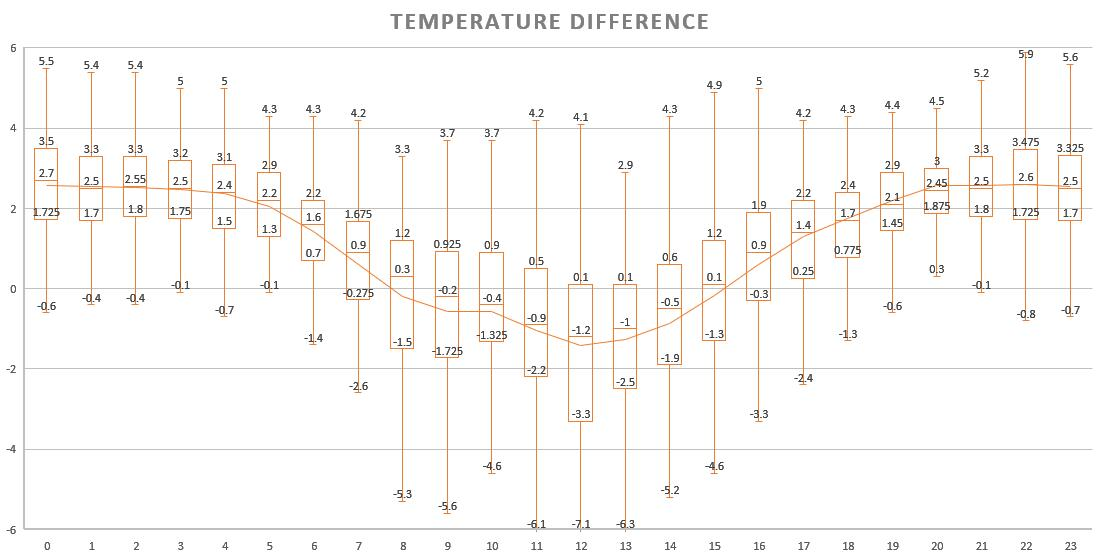
\includegraphics[scale=0.55]{HeatIsland_Construction.jpg}
				\caption{Temperature Difference Between the Measured Station Temperature and the Measured Site Temperature }
				\label{fig:HeatIslandConst}
				\end{figure}
				
				\begin{figure}[H]
				\centering
				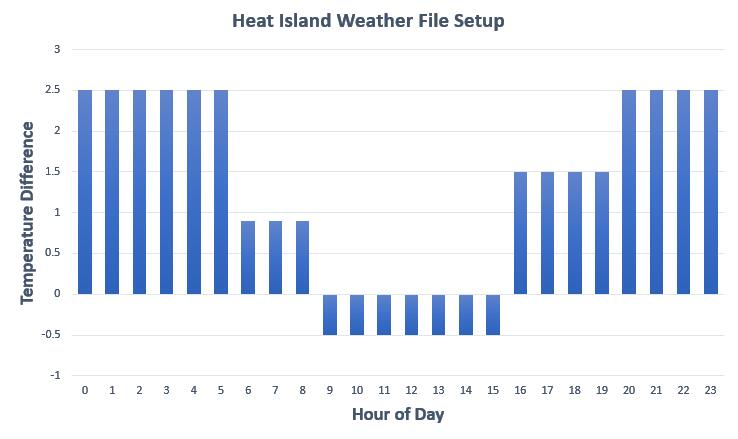
\includegraphics[scale=0.75]{HeatIslandConstruction.jpg}
				\caption{Heat Island Temperature Modification Rule}
				\label{fig:HeatIslandRule}
				\end{figure}
				



	\section{Static Calculation}
		To investigate the cause of huge deviation between previous static calculation and measured heating demands, a new static calculation is conducted with more accurate geometry and weather information. As static calculation follows the standard method proposed by SIA 380/1. Overall, the heating demand is obtained by subtracting heat losses with heat gains. The SIA calculation is divided into several parts. Each part calculates a type of energy loss or energy gain. \\
		\[\text{Heating Demand} = \text{Heat Losses} - \text{Heat Gains}\]
		
		\textbf{Losses}\\
			The standard calculation method SIA 380/1 takes a number of losses into account, mainly \textit{transmission loss} and \textit{ventilation loss}. The \textit{transmission loss} includes heat loss through conduction, heat loss through convection, and heat loss through thermal bridge. The losses are calculated based on the building location's heating degree days, building material thermal properties, and the dimension of building elements. The formula for the losses are given in appendix \ref{sec:siacalculation}.\\

		\textbf{Gains}\\
			In SIA 380/1 calculation, heat gains are obtained from solar radiations, internal gains by electronics, and internal gains by occupant activities. A detailed calculation formular set is also provided in Appendix \ref{sec:siacalculation}.\\
			
		\textbf{Measurements expected to close the performance gap}
			The building model is firstly subject to static calculation with all standard values and assumptions. After the reference static calculation has been made, another calculation with 2015 weather information is conducted. Depend on the obtained result, further parameters are modified and try to match the calculation results with the measured annual results.

		
	\section{Dynamic Calculation}
		The dynamic analysis include a time-step calculation considering the step change of building thermal information. Therefore, EnergyPlus is used to provide an hourly analysis of the two buildings. A detailed setup of parameters are given below.
		
		The occupancy schedule and activity level of all zones of the two buildings are from the SIA 2024 standard. The SIA 2024 standard provides a guideline assumptions for different building areas such as bedroom, bathroom, kitchen, office, and corridor.\\

		The detailed information of is stored in separate .\textit{csv} files which contains 8760 entries of hourly data. Below is a list of information obtained from SIA 2024.

	\begin{itemize}
		\item Heating/Cooling Setpoint temperature ($^oC$)
		\item Occupancy schedule \& occupant density ($m^2/\text{person}$)
		\item Activity level (W/m$^2$)
		\item Lighting Schedule
		\item Lighting Level ($W/m^2$)
		\item Domestic hot water schedule 
		\item Domestic hot weater level ($W/m^2$)
		\item Electricity appliance schedule
		\item Electricity appliance level ($W/m^2$)
	\end{itemize}


		Figure \ref{fig:HeatingSP} below shows the nominal heating setpoints of all zones. Most schedules and activities have a certain weekday/weekend pattern and have different patterns in different months. Figure \ref{fig:JanOffice_Vent} below shows the office ventilation schedule on weekdays in January. The schedule is presented as a percentage of the nominal level in Norm SIA 2024.\\
		
		\begin{figure}[H]
		\centering
		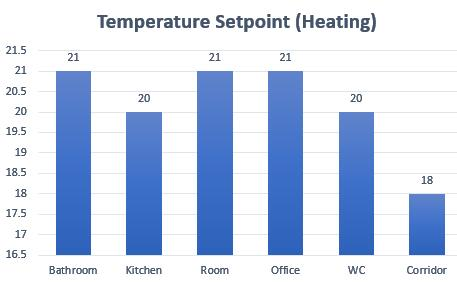
\includegraphics[scale=1.1]{TempSetpoint.jpg}
		\caption{Heating Temperature Set point}
		\label{fig:HeatingSP}
		\end{figure}
		


		\begin{figure}[h!]
		\centering
		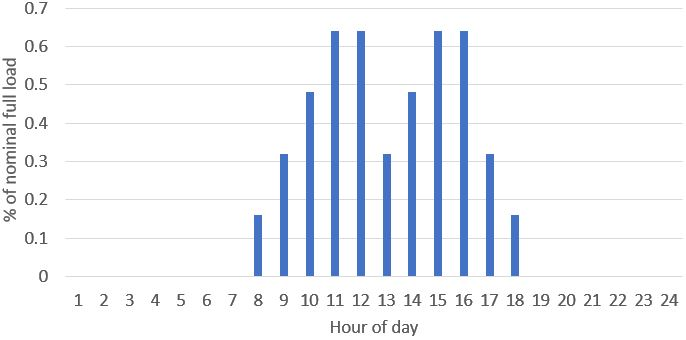
\includegraphics[scale=0.8]{figures/JanOffice_Vent.jpg}
		\caption{Office Ventilation Schedule in January Weekday}
		\label{fig:JanOffice_Vent}
		\end{figure}
		
	\section{Calibration}
		In order to ensure the simulated buildings have similar thermal behaviors as the real buildings, a calibration for the building envelope properties is needed. The calibration process needs to be in a summer period where no heating and cooling is performed. The calibration process varies the building air tightness, internal loads, and user behaviors until the calculated indoor temperature behaves similar enough to the measured data. Lastly, the calibrated building is again subject to annual analysis and aim to match the calculated annual energy consumption with the actual measured value.\\
		
		

		\textbf{Building Envelope Calibration}\\
			The air tightness is thought to be an important factor in building simulation. Therefore, the calibration process would vary the air tightness between 0.1 to 0.5 ach and try to match both the hourly indoor temperature as well as the annual heating demand.\\


		\textbf{Internal Loads}\\
			Internal load such as lighting and appliance schedule can change the indoor temperature pattern. Therefore, in the calibration process, lighting schedule and electricity schedule are modified to observe the indoor temperature of the focused non-heating period. The newly generated schedules should be separated into weekday and weekend schedule.\\


		\textbf{User behavior}\\
			The user behavior is also thought to be an influential factor to indoor comfort. The calibration also investigate the control strategies for users to operate the window shading. A number of shading controls is used and the strategy with most similar indoor temperature patten is used in the calibrated model. The newly constructed shading schedule should vary between summer and winter schedule.\\


	\section{Parameters Variation}
		
		\textbf{Simulation Tool}\\
		\textit{jE-Plus} is used as a tool to coordinate the analysis by sampling different values for the varied parameters \& perform different EnergyPlus simulations using them. jEPlus is also able to collect the relevant results from all simulations. In total, 1000 simulations are performed in the parameter variation analysis.\\
		
		\par
		\textbf{Parameters}\\
		After the building model has been constructed and calibrated, a further analysis with varied parameters can be performed. Following a similar approach from Mavromatidis \cite{GeorgeThesis}, Ioannou and Itard \cite{ioannou2015energy}, Table \ref{tab:ParameterDistribution} shows the parameters that are focused and subject to variation in this thesis:\\

	\begin{table}[htbp]
    	\centering
    	\small
    	\caption{Uncertainty distributions for parameters related to building energy demands \cite{GeorgeThesis}}
    	    \begin{tabular}{|c|c|c|}

			\toprule
			Parameter           & probability distribution & Distribution parameters \\
			\hline
			Material Properties & \makecell{Normal distribution \\ $N(\mu,\sigma)$} & \makecell{$\mu = \text{norminal value}$\\$\sigma=0.1 \cdot \mu$}\\
			\hline
			Infiltration (ACH)  &\makecell{Normal distribution \\ $N(\mu,\sigma)$} & \makecell{$\mu = \text{norminal value}$\\$\sigma=0.1 \cdot \mu$}\\
			\hline
			\makecell{Occupancy density\\(m$^2$/person)} & \makecell{Triangular distribution \\ $\tau(\alpha,\beta,\gamma)$}  & \makecell{$\alpha = $ SIA2024-min \\ $\beta = $ SIA2024-nominal \\ $\gamma = $ SIA2024 -max} \\
			
			\hline
			
			\makecell{Lighting capacity\\(W/m$^2$)} & \makecell{Triangular distribution \\ $\tau(\alpha,\beta,\gamma)$}  & \makecell{$\alpha = $ SIA2024-min \\ $\beta = $ SIA2024-nominal \\ $\gamma = $ SIA2024 -max} \\
			\hline
			\makecell{Equipment capacity\\ (W/m$^2$)}& \makecell{Triangular distribution \\ $\tau(\alpha,\beta,\gamma)$}  & \makecell{$\alpha = $ SIA2024-min \\ $\beta = $ SIA2024-nominal \\ $\gamma = $ SIA2024 -max} \\
			\hline
			
			\makecell{Hot water demand\\(W/m$^2$)} & \makecell{Triangular distribution \\ $\tau(\alpha,\beta,\gamma)$}  & \makecell{$\alpha = $ SIA2024-min \\ $\beta = $ SIA2024-nominal \\ $\gamma = $ SIA2024 -max} \\
			\hline
			\makecell{Ventilation rates\\(m$^3$/h/person)} & \makecell{Normal distribution \\ $N(\mu,\sigma)$}      & \makecell{$\mu = \text{norminal value}$\\$\sigma=0.1 \cdot \mu$}                       \\
			\hline
			
			\makecell{Thermostat setting\\($^oC$)} & \makecell{Normal distribution \\ $N(\mu,\sigma)$}      & \makecell{$\mu = \text{norminal value}$\\$\sigma= 1 ^oC$}\\
			\hline

			\makecell{External heat transfer coefficient \\ (W/m$^2K$)} & \makecell{Uniform distribution \\ $N(a,b)$}      & \makecell{$a = 90\%\text{ norminal value}$\\$b = 110\% \text{ nominal value}$}\\
			
			\hline

			\makecell{Internal heat transfer coefficient \\ (W/m$^2K$)} & \makecell{Normal distribution \\ $N(\mu,\sigma)$}      & \makecell{$a = 90\%\text{ norminal value}$\\$b = 110\% \text{ nominal value}$}\\
			\hline
			\makecell{Facade solar absorptance} & \makecell{Uniform distribution \\ $U(a,b)$}      & \makecell{$a = \text{0.2}$\\$b= 0.9$}\\
			
			\bottomrule
        	\end{tabular}%
        	\label{tab:ParameterDistribution}%
    \end{table}%			
			
			

		\textit{Heating Temperature Setpoint}\\
			All zones' heating setpoint temperature are part of the parameter variation. The heating setpoint temperature for the same category at the same floor are thought to be identical. For example, the heating setpoint temperature of \textit{Room2} and \textit{Room3} at the second floor would be the same, but might be different to the heating setpoint temperatues for \textit{Room2} and \textit{Room3} at third floor.\\
			The heating temperature setpoint is at a normal distribution with mean value $\mu =$ nominal value and the diviation $\sigma = 1 ^oC$. The range of temperature setpoint samples in this thesis for each zones is shown in Figure \ref{fig:TempSetpoint}. The temperature setpoint is randomly created in a normal distribution with the given mean and standard deviation values.\\

			\begin{figure}[H]
			\centering
			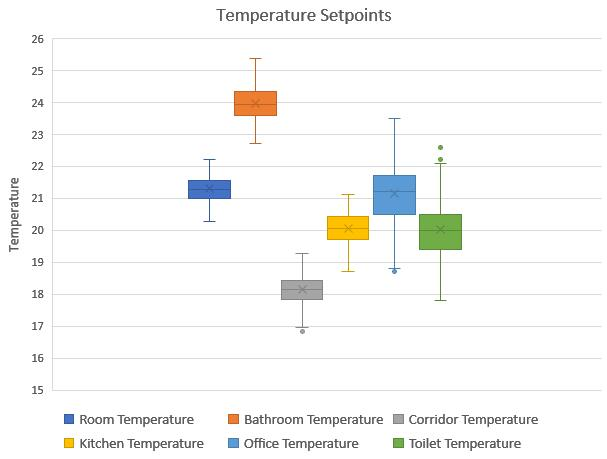
\includegraphics[scale=0.85]{Residential_TempSetpoint.jpg}
			\caption{Heating Temperature Setpoint Distribution}
			\label{fig:TempSetpoint}
			\end{figure}
		
		\textit{Occupancy Level}\\
			The zone occupancy level is given by $m^2/\text{person}$. A triangular distribution is used where the minimum value $a$, the nominal value $b$, and the maximum value $b$ are defined in SIA 2024, as shown in Table \ref{tab:ParameterDistribution}. For example, Figure \ref{fig:HonggRoomOcc} shows the room occupancy level

			\begin{figure}[h!]
			\centering
			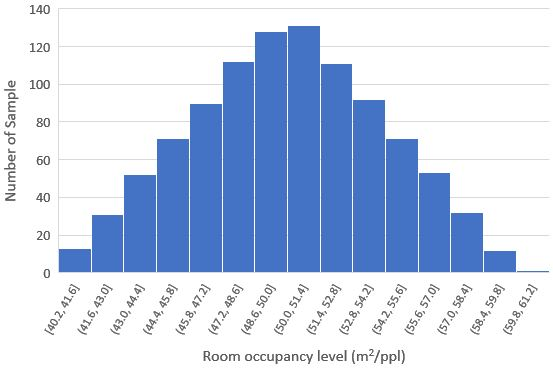
\includegraphics[scale=0.9]{figures/RoomOccupancy.JPG}
			\caption{Room Occupancy Level of Residential Building}
			\label{fig:HonggRoomOcc}
			\end{figure}
			
		\textit{Lighting Level}\\
			The zone lighting level is given by a triangular distribution with detailed parameter settings shown in norm SIA2024. A box plot is given in Figure \ref{fig:LightingDistribution} to indicate the distribution of the lighting level setpoints.\\

			\begin{figure}[h!]
			\centering
			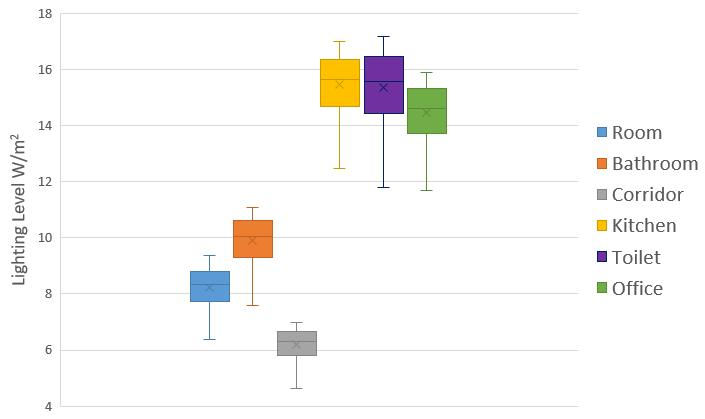
\includegraphics[scale=0.7]{figures/LightingLevelDistribution.jpg}
			\caption{Lighting Level Distribution for all zones}
			\label{fig:LightingDistribution}
			\end{figure}

		\textit{Appliance Level}\\
			The zone appliance level is given by a triangular distribution with detailed parameter settings shown in norm SIA2024. A box plot is given in Figure \ref{fig:ApplianceDistribution} to indicate the distribution of the lighting level setpoints. SIA 2024 assume a 0 appliance level in corridor, bathroom and toilet area, therefore only 3 zones are shown in the figure. \\
			\begin{figure}[h!]
			\centering
			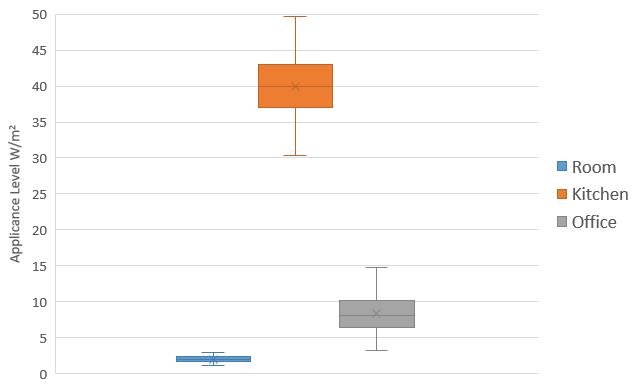
\includegraphics[scale=0.7]{figures/ApplianceLevelDistribution.jpg}
			\caption{Appliance Level Distribution for all zones}
			\label{fig:ApplianceDistribution}
			\end{figure}

		\textit{Domestic Hot Water Level}\\
			The zone appliance level is given by a triangular distribution with detailed parameter settings shown in norm SIA2024. A box plot is given in Figure x to indicate the distribution of the lighting level setpoints.\\


			\begin{figure}[h!]
			\centering
			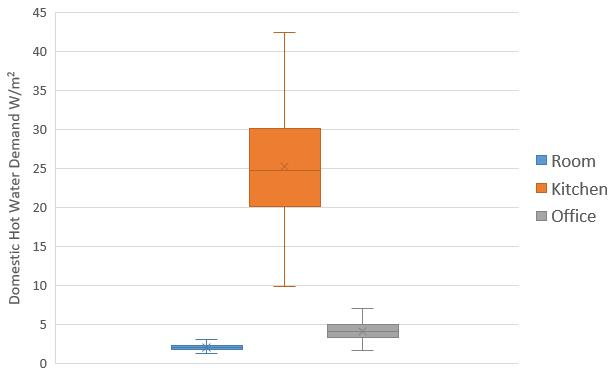
\includegraphics[scale=0.7]{figures/DHWLevelDistribution.jpg}
			\caption{DHW Level Distribution for all zones}
			\label{fig:DHWDistribution}
			\end{figure}
		


		\textit{Ventilation Level}\\
			Similarly, the ventilation level for each zone is given in Figure \ref{fig:VentLevel}. The ventilation level for the same zone category at the same floor are thought to be identical. The ventilation level varies according to a normal distribution rule as shown in Figure \ref{fig:VentDist}.\\

			\begin{figure}[ht!]
			\centering
			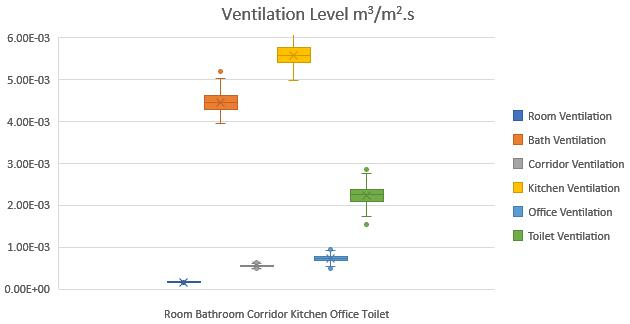
\includegraphics[scale=0.6]{Ventilation_Level.jpg}
			\caption{Ventilation Level Distribution for different building room types}
			\label{fig:VentLevel}
			\end{figure}

			\begin{figure}[ht!]
			\centering
			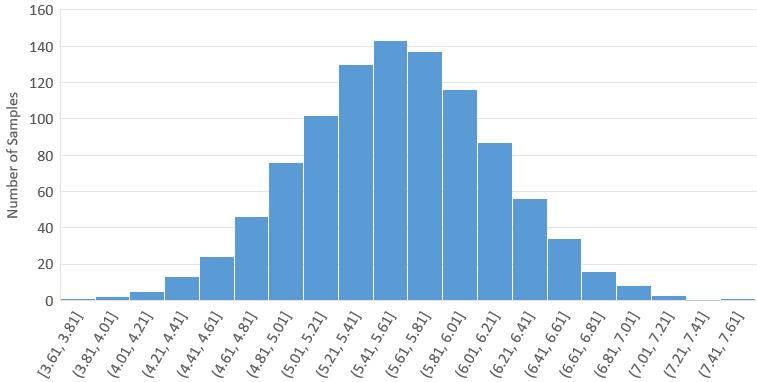
\includegraphics[scale=0.65]{Kitchen_Vent.jpg}
			\caption{Air Ventilation Distribution for Kitchen (in 0.001 $m^3/m^2 \cdot s$)}
			\label{fig:VentDist}
			\end{figure}
						
		\textit{Infiltration}\\
			The infiltration level is roughly a normal distribution which takes the nominal infiltration as mean value $\mu$, and the deviation $\sigma = 10\% \cdot \mu$. Figure \ref{fig:EXPAirInfiltration_Sumatra} shows an example air infiltration distribution.\\

			\begin{figure}[ht!]
			\centering
			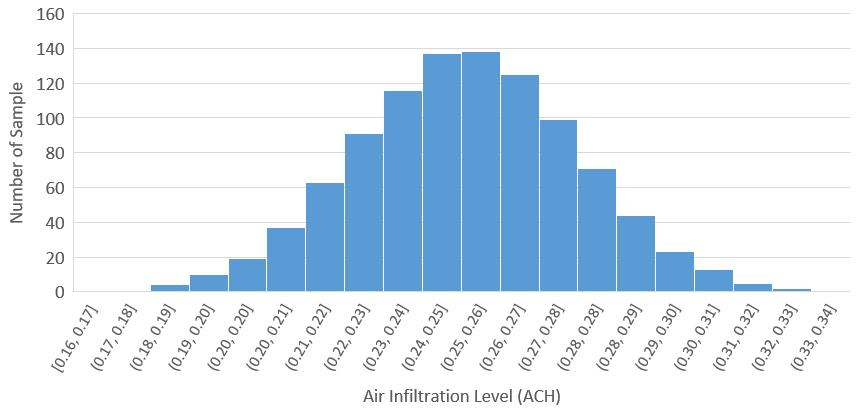
\includegraphics[scale=0.65]{Example_Normal_Distribution.jpg}
			\caption{Example Air Infiltration Distribution (with $\mu = 0.25$, $\sigma = 10\% \mu$)}
			\label{fig:EXPAirInfiltration_Sumatra}
			\end{figure}
		
		\textit{Internal and External convection coefficient}\\
			The internal and external convection coefficient range between $\pm 10\%$ of the nominal value.
			A uniform distribution is applied, means the probability of the convection coefficient being any number between $\pm 10\%$ of the nominal value is the same. Figure \ref{fig:HonggerIntConvDist} and Figure \ref{fig:HonggerExtConvDist} shows a distribution histogram of the internal and external heat convection coefficient.\\

			\begin{figure}[ht!]
			\centering
			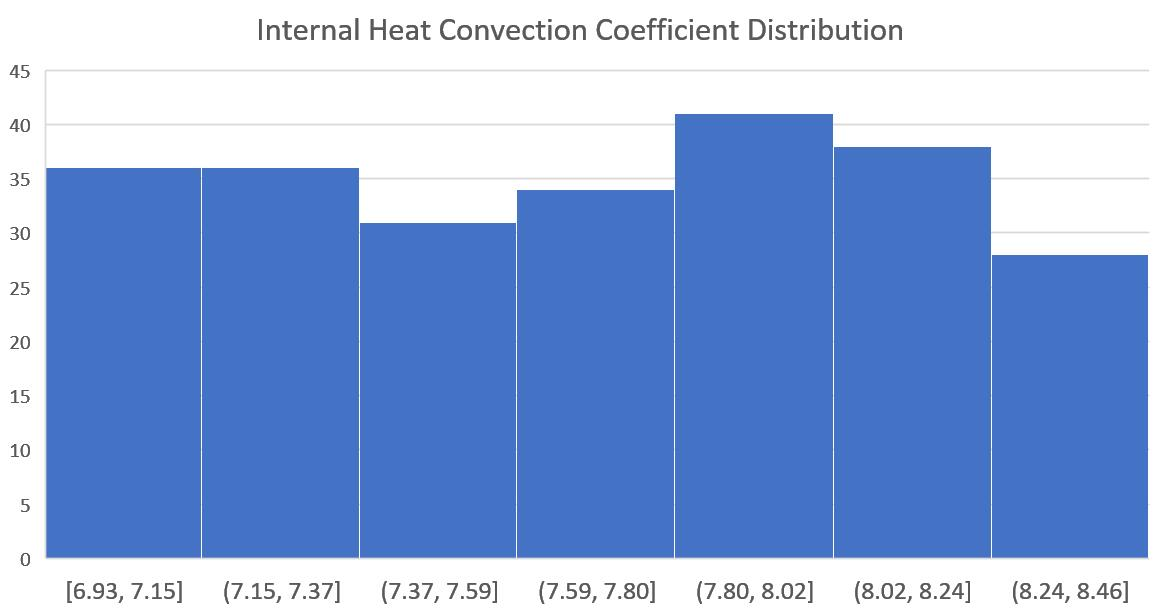
\includegraphics[scale=0.35]{Hongger_InConvDist.jpg}
			\caption{Internal Heat Convection Coefficient Distribution}
			\label{fig:HonggerIntConvDist}
			\end{figure}
			
			\begin{figure}[ht!]
			\centering
			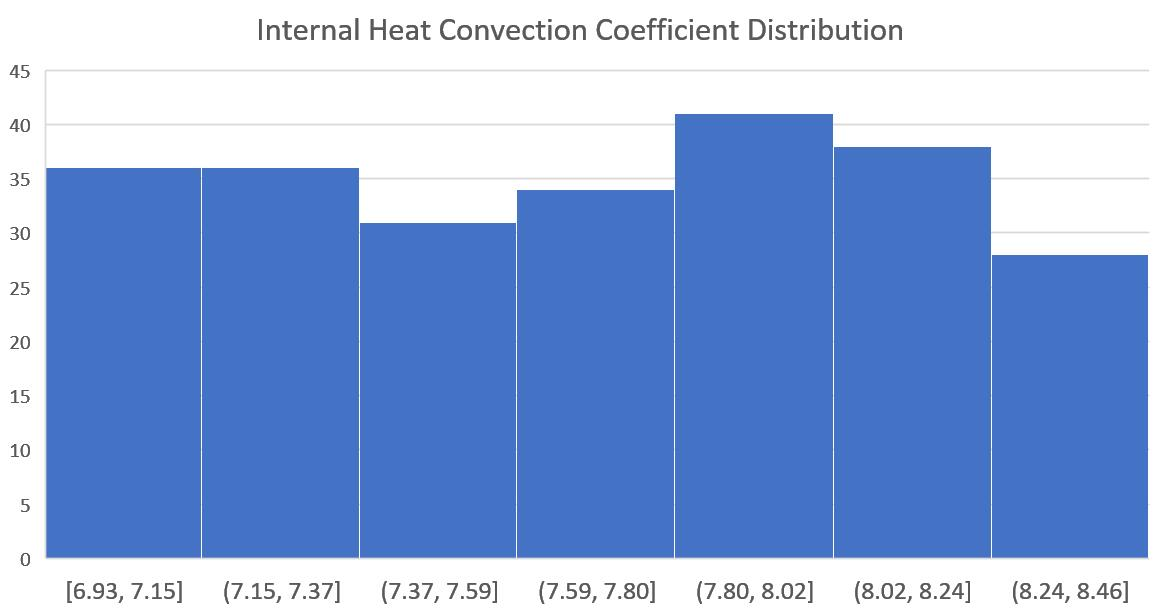
\includegraphics[scale=0.35]{Hongger_InConvDist.jpg}
			\caption{External Heat Convection Coefficient Distribution}
			\label{fig:HonggerExtConvDist}
			\end{figure}
			
		\textit{Facade solar absorptance}\\
			The facade paint and facade color determine the facade solar absorptance. It range from 0 to 1 where a 0 absorptance means the surface reflex all the energy onto the surface, and a 1 absorptance means the facade absorb all the solar energy onto the surface. In this analysis the solar absorptance vary between 0.2 to 0.9 at a discrete distribution.

	\section{Data Processing}
		\textit{Python} and Excel are used in processing the results, where excel is used to generate histograms and other regular charts, while Python (with Matplotlib package) is used to merge data sets, process a series of data files, generate other irregular charts such as correlation matrix, and some boxplots.

		\subsection{Dynamic Analysis Range}
			Histogram and boxplots are used to show the distribution and the range of the dynamic analysis results after the parameter variation. A box focuses on the effect of different simulation environments or parameters, while a histogram focuses more on the range and the distribution of a single variable.

		\subsection{Correlation Matrix}
			In order to display the relations between input parameters and the relations between input parameters and heating demands and DHW demands, a correlation matrix is needed to show their influence on each other. \\
			Essentially, the correlation matrix is a heat map matrix where a deeper color represents a higher absolute value. Correlation range between -1 to 1, where -1 and 1 represent a perfect linear relationship and 0 indicates that there is no association between two variables.\\
		

\chapter{Results}

	\section{Static Calculation}
		The results of static calculation are shown in the following sections. Firstly the results of office building then the residential building results at each steps are shown below according the methodology. A summary is also given after each energy loss and energy gain section is presented.\\

		Figure \ref{fig:Sumatra_SIA} and Figure \ref{fig:Hongger_SIA} show the static calculation results based on SIA 380/1 standard. The first bar from the left shows the result from a previous report given by \textit{Lemon Consult} \cite{SIAPreviousreport}, the calculation is using the gross floor area which external walls and internal partitions are included. The second bar represent the result from a corrected building envelop, which net area is used and the external walls and internal partitions are excluded from the floor area calculation. The results show a significant drop in heating demand after using internal net area instead of gross area, which may indicate that net area is a better parameter in SIA 380/1 calculation than gross area.\\

		The third bar represents a calculation result from changing the SIA 381/2 stand weather condition to the actual 2015 weather condition from Zurich NABZUE station. From the previous chapter, it is clear that the overall temperature in 2015 is much warmer than the standard SIA 381/2 weather assumption, which may become a major reason of heating energy overestimation and a huge performance gap. The results from both the office building and the residential building indicate a significant performance gap improvement after the year 2015 actual weather condition is used. Therefore, it indicates that in macroscopic view, SIA 380/1 calculation standard can achieve a much smaller performance gap by using the net floor area and an accurate weather condition. 

		\begin{figure}[htbp]
		\centering
		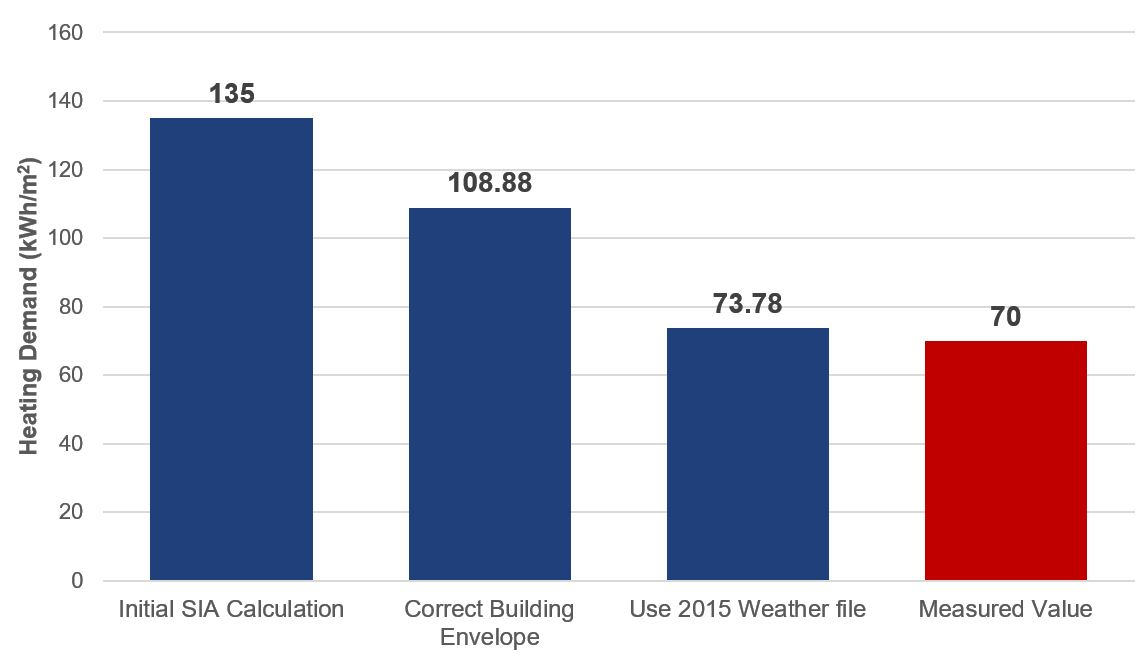
\includegraphics[scale=0.46]{Office_SIA.jpg}
		\caption{SIA Calculation Improvement for Office Building}
		\label{fig:Sumatra_SIA}
		\end{figure}
		
		\begin{figure}[htbp]
		\centering
		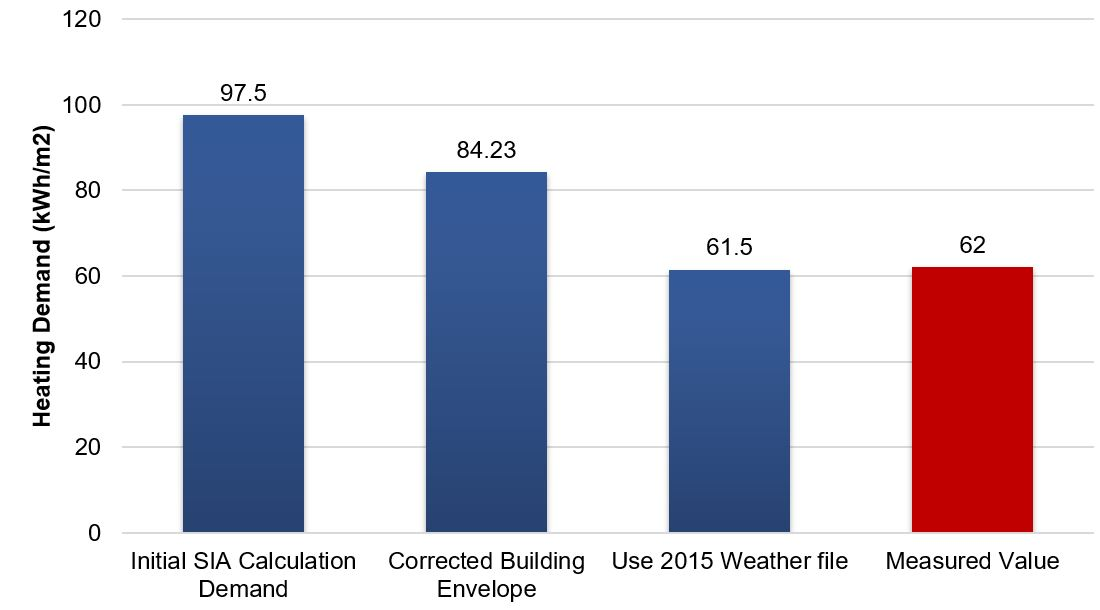
\includegraphics[scale=0.46]{Residential_SIA.jpg}
		\caption{SIA Calculation Improvement for Residential Building}
		\label{fig:Hongger_SIA}
		\end{figure}
		
		
	\newpage		  
	\section{Dynamic Simulation}		
			The dynamic simulation results are shown below in Figure \ref{fig:Sumatra_EP} and Figure \ref{fig:Hongger_EP} below. Firstly, the simulation is run in 2015 weather conditions and with standard building envelope, which is shown in the first bar from the left. Secondly, the air change ratio is changed from 0.1 ACH to a more realistic value of 0.3 ACH, which is shown in the second bar from the left. Then, the third bar shows the results after SIA standard heat convection coefficient values are applied on the model. The result shows a close match between the calculated heating demand and the measured heating demand. It appears that both buildings can obtain a very close estimation when using these approaches. However, in order to further verify the building simulation methods and parameters, a building calibration is needed for both buildings.
		

		\begin{figure}[htbp]
		\centering
		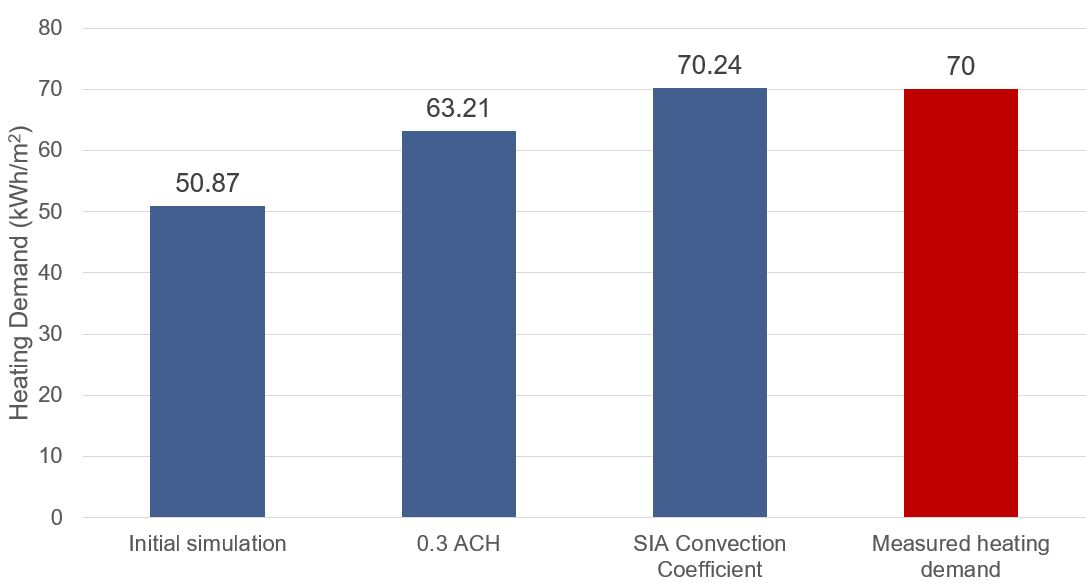
\includegraphics[scale=0.5]{Office_EP.jpg}
		\caption{Office Building Dynamic Calculation Correction}
		\label{fig:Sumatra_EP}
		\end{figure}

		\begin{figure}[htbp]
		\centering
		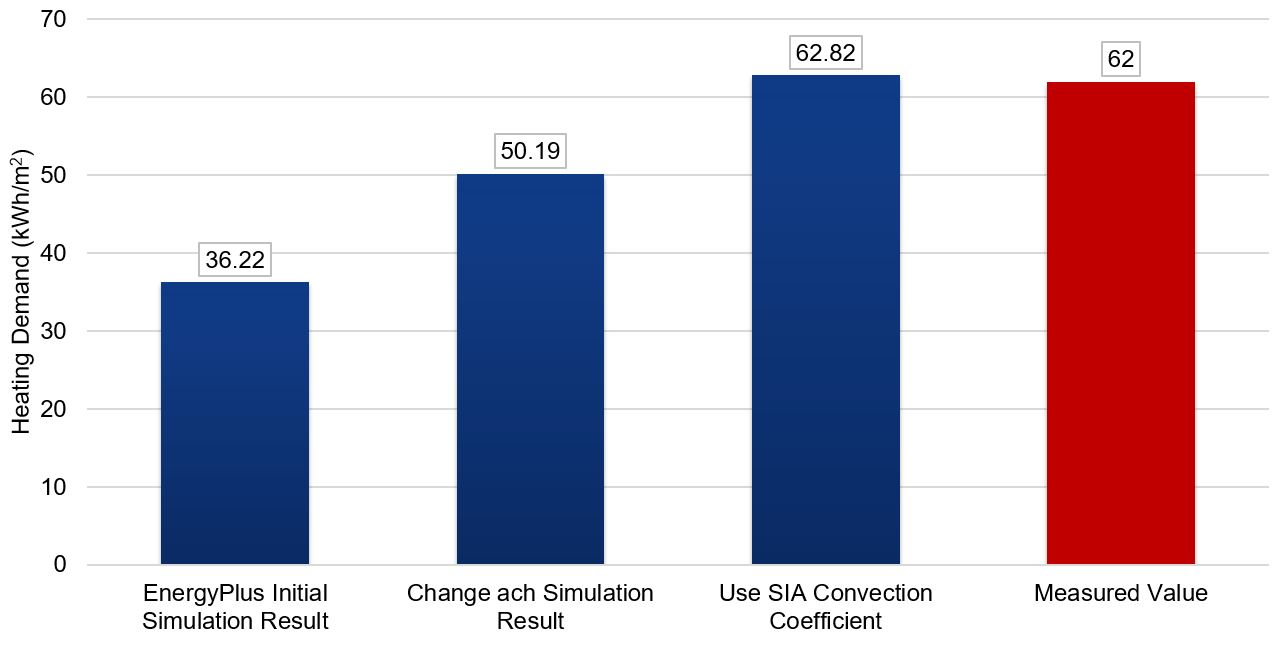
\includegraphics[scale=0.4]{Residential_EP.jpg}
		\caption{Residential Building Dynamic Calculation Correction}
		\label{fig:Hongger_EP}
		\end{figure}
		
		



	\newpage
	\section{Calibration Results}

			Figure \ref{fig:ACH_Compare} shows a comparison of average calculated indoor temperature from 1$^{st}$ June to 10$^{th}$ June in 2015 in the residential building under different air tightness (0.1/0.3/0.5 air change per hour infiltration level). The blue line with huge fluctuation represents the outdoor temperature from the weather station, the red line represents the measured indoor temperature, and the gray, orange, and orange line represent the calculated indoor temperature of the three rooms at the same apartment. The result indicates that the air infiltration dose not have a strong impact on indoor temperature profile. Therefore, the air infiltration is used to calibrate the annual heating demand to the measured value after the temperature profile is matched. The result also indicates that the simulated indoor temperatures are more fluctuated than the measured actual value, which is probably due to some wrong assumptions on building operations or user behavior.\\
		
			\begin{figure}[H]
			\centering
			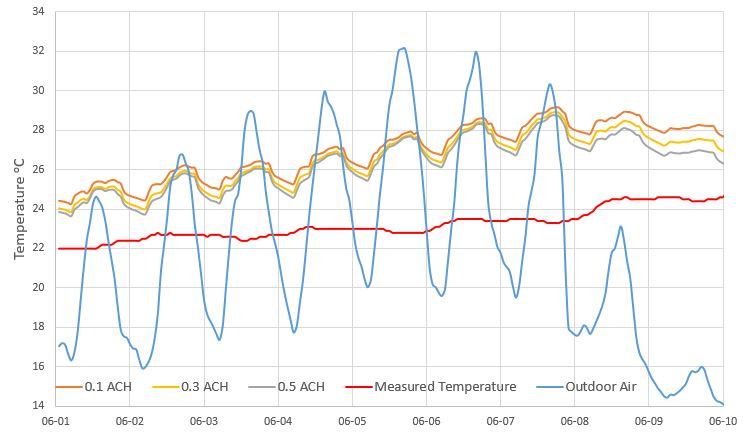
\includegraphics[scale=0.75]{ACH_Compare.JPG}
			\caption{Temperature Profile (Average) Comparison Between Different (0.1/0.3/0.5) ACH Values}
			\label{fig:ACH_Compare}
			\end{figure}

			\begin{figure}[H]
			\centering
			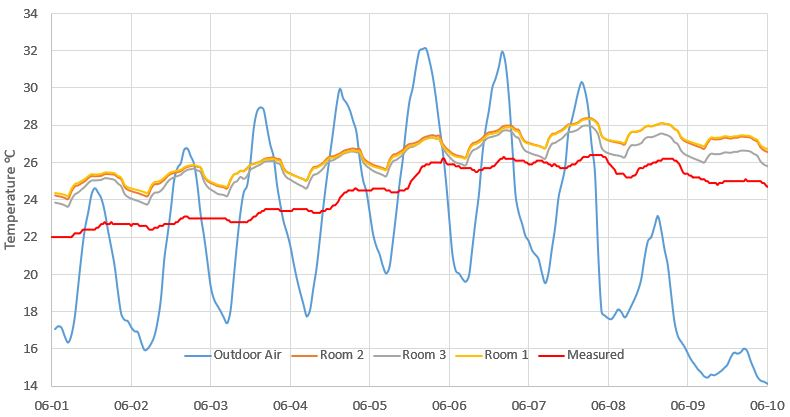
\includegraphics[scale=0.7]{figures/Hongg_Clibration_Origin.JPG}
			\caption{Origin Temperature Profile of Residential Building}
			\label{fig:HonggCalibrationOrigin}
			\end{figure}
			
			Figure \ref{fig:HonggCalibrationOrigin} shows a temperature profile of the first floor apartment with 0.3 ACH infiltration. The light blue line with huge fluctuation is the outdoor temperature measured by the weather station. The The less fluctuated dark blue line represents the measured indoor temperature. The rest lines in grey, yellow and red represent the calculated indoor temperature of three bedrooms within the apartment. This origin temperature profile indicates an over-estimation on heat gains. Therefore, the calibration process aimed on reducing the internal gains by varying the building electronic appliance and lighting schedules.\\
			
			\begin{figure}[H]
			\centering
			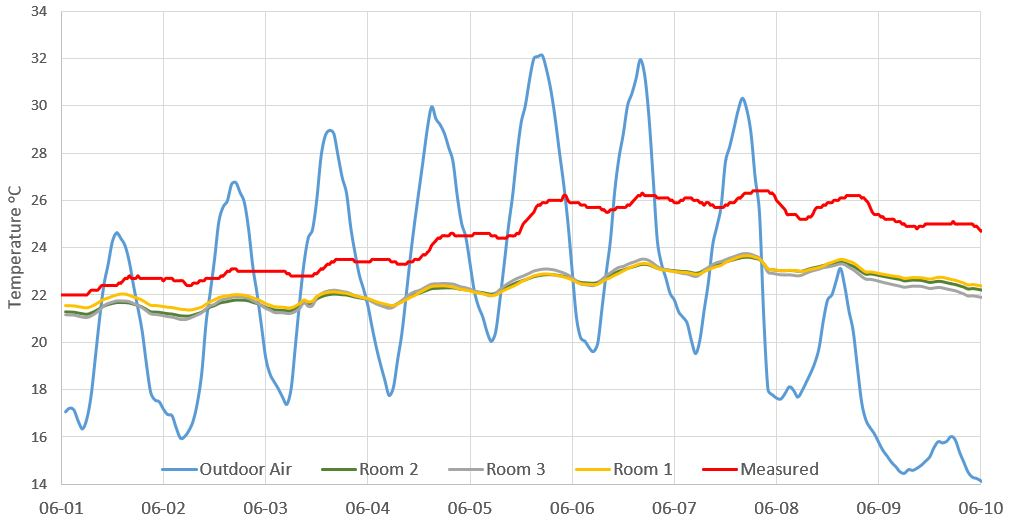
\includegraphics[scale=0.57]{figures/Hongg_Cali_NoFacility.JPG}
			\caption{Temperature Profile of Residential Building Without Internal Gains}
			\label{fig:HonggCalibrationNoGains}
			\end{figure}
			
			In order to verify the above conclusion, another simulation is taken with no electronic appliance and lighting. The result in Figure \ref{fig:HonggCalibrationNoGains} proved that the wrong appliance and lighting assumption schedule is the cause of this over-heating problem. The room temperature dropped around 4 degrees when all the appliances are turned off. When carefully checking the lighting schedule and electronic appliance provided by SIA 2024 schedule, it found that the lighting schedule and lighting level are well over estimated for residential buildings. Therefore, the residential buildings are modified as Table \ref{tab:HonggLightingCtrl}. \\

			\begin{figure}[H]
			\centering
			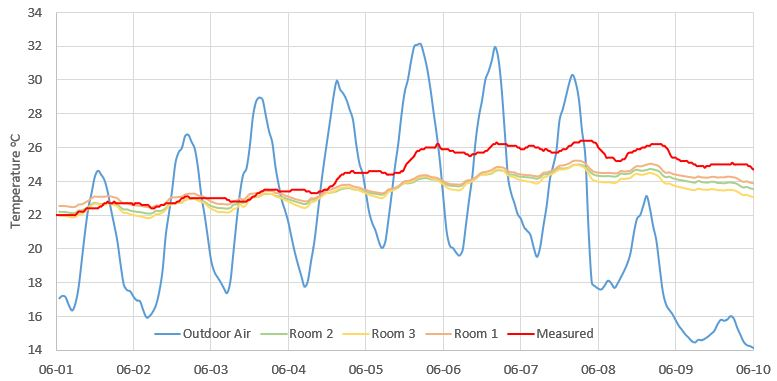
\includegraphics[scale=0.75]{Hongg_Clibration_03NoLight.JPG}
			\caption{Temperature Profile of Residential Building with No Lighting}
			\label{fig:HonggerCalibrationNoLight}
			\end{figure}

			Figure \ref{fig:HonggerCalibrationNoLight} above shows the temperature profile without lighting. The highly fluctuated blue line represents the outdoor temperature, the red line represents the actual measured data, and the orange, yellow, and light green lines represent  the calculated indoor temperature of three rooms. The result again indicated that the lighting schedule is the main cause of over-heating. Therefore, a new lighting schedule is created and rerun the simulation under a new lighting schedule. The new lighting schedule can be found in Table \ref{tab:HonggLightingCtrl} below.
			
        	\begin{table}[htbp]
        	\centering
        	\caption{New Lighting Schedule}
        	    \begin{tabular}{ccc}
        	    \toprule
        	    Lighting Schedule & Weekday & Weekend\\
        	    \midrule
                Until 02:00 & 0.05 & 0.05 \\
                Until 06:00 & 0.03 & 0.03\\
                Until 09:00 & 0.5 & 0.3\\
                Until 17:00 & 0.2 & 0.2\\
                Until 22:00 & 0.7 & 0.7\\
                Until 22:00 & 0.7 & 0.7\\
                Until 24:00 & 0.2 & 0.5\\
        	    \bottomrule
        	    \end{tabular}%
        	  \label{tab:HonggLightingCtrl}%
        	\end{table}%			
			
			
			\begin{figure}[H]
			\centering
			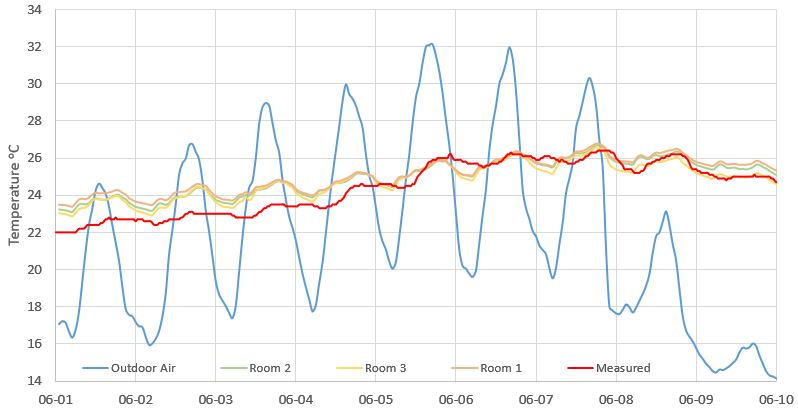
\includegraphics[scale=0.7]{Hongg_Clibration_03NewLight.JPG}
			\caption{Temperature Profile of Residential Building with New Lighting Schedule}
			\label{fig:HonggerCalibrationNewLight}
			\end{figure}
			
			When applying the new lighting schedule and keeping the appliance schedule as it is, the calibration result is shown in Figure \ref{fig:HonggerCalibrationNewLight}. The result shows a temperature profile estimation very close to the measurement value, and the indoor temperature can be claimed as completed.
			The origin air infiltration level is 0.3 ACH. However, the annual heating demand indicates that this setting has higher demand than the measured value. Therefore, the air infiltration is slightly decreased to 0.25 ACH in order to fit the annual heating demand.\\ 

			\textbf{Office Building Calibration}\\
			Similarly, the office building went through a calibration process with the same approach. Firstly, the simulation is taken without any modification. An overheating is observed from the temperature profile. As the building is mostly covered with window on the west and south side, applying shading control would probably solve the problem. To test the effect of window shadings, another simulation is done under 24/7  on shading schedule. The results in Figure \ref{fig:Sumatra_Calibration_Allshade} indicates that the shading of the actual building is mainly on, as the calculated temperature profile behaved very similar with the measured temperature profile. Therefore, it can assume that the blinds at the office building is mainly on at non-heating period. While in winter period, a modest blind control is applied and the annual heating demand is observed.

			\begin{figure}[H]
			\centering
			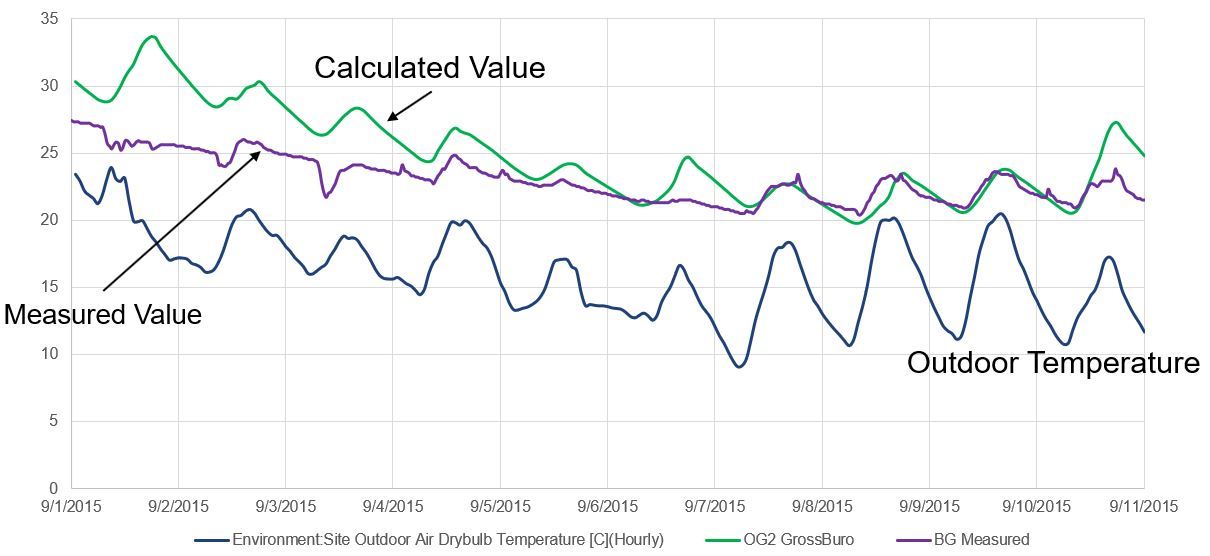
\includegraphics[scale=0.70]{figures/Office_Calibration_Ori.JPG}
			\caption{Origin Temperature Profile of Office Building}
			\label{fig:Sumatra_Calibration_Ori}
			\end{figure}
			
			\begin{figure}[h!]
			\centering
			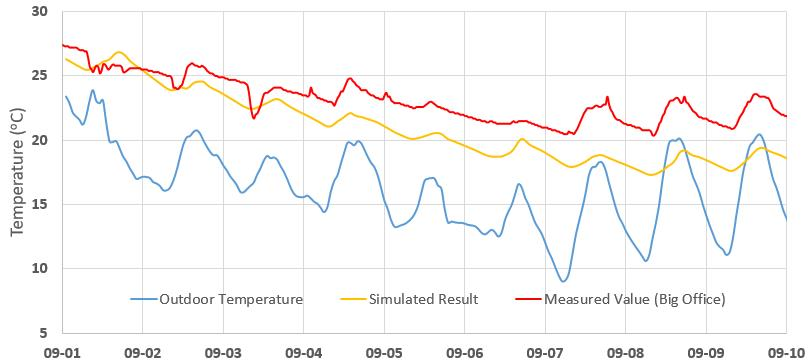
\includegraphics[scale=0.7]{Sumatra_Calibration_AllonShading.JPG}
			\caption{Temperature Profile of Office Building with 24/7 shading}
			\label{fig:Sumatra_Calibration_Allshade}
			\end{figure}			
			
			Table \ref{tab:HonggShadingCtrl} below shows a new shading control schedule in both summer and winter. Another simulation is taken after the new shading schedule is applied on the model. The result in Figure \ref{fig:Sumatra_Calibration_NewShading} below shows an identical pattern as Figure \ref{fig:Sumatra_Calibration_Allshade} in summer period. The annual heating demand for office building with different air infiltration and total ventilation level is shown below at Table \ref{tab:SumatraVentLevel}. As the measured total heating consumption was around 70 $kWh/m^2$, the air infiltration is then calibrated to 0.1 ACH.\\
			
		\begin{table}[htbp]
		\centering
		\caption{New Shading Control Schedule}
		    \begin{tabular}{ccc}
		    \toprule
		    Blind Schedule & Summer & Winter\\
		    \midrule
            Weekday & Always on & 10:00 - 16:00 \\
            Weekend & Always on & Always off\\
		    \bottomrule
		    \end{tabular}%
		  \label{tab:HonggShadingCtrl}%
		\end{table}%
            
            
		\begin{table}[htbp]
		\centering
		\caption{Annual Heating Demand of Office Building for Different Ventilation Levels}
		    \begin{tabular}{ccc}
		    \toprule
		    Infiltration Level (ACH) & Total Outdoor Air (ACH) & Heating Demand ($kWh/m^2$)\\
		    \midrule
            0.1 & $\approx$ 0.87 & 71.87\\
            0.2 & $\approx$ 0.97 & 77.97\\
            0.3 & $\approx$ 1.07 & 84.18\\
            
		    \bottomrule
		    \end{tabular}%
		  \label{tab:SumatraVentLevel}%
		\end{table}%
		
		
            \begin{figure}[H]
			\centering
			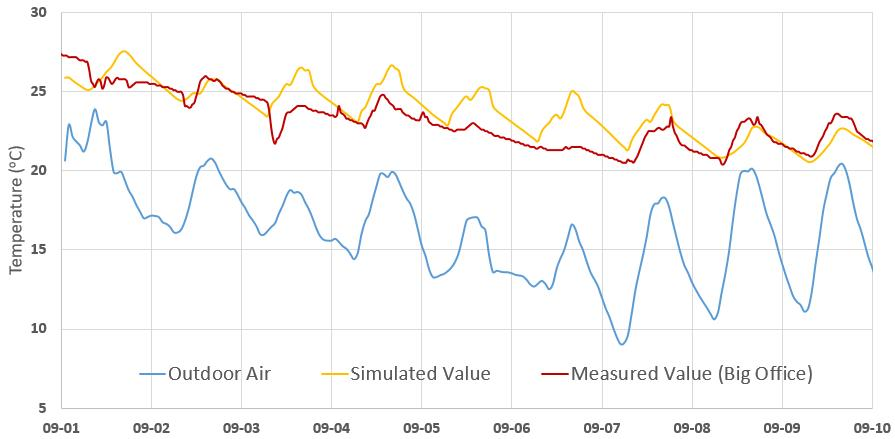
\includegraphics[scale=0.65]{Sumatra_Calibration_NewShading.JPG}
			\caption{Temperature Profile of Office Building with new shading schedule}
			\label{fig:Sumatra_Calibration_NewShading}
			\end{figure}
	
	\newpage	
	\section{Parameters Variation Results}

		The parameters variation processes can be done after the buildings are calibrated. The results are presented in a form of histograms and correlation matrices. The histogram helps understand the range of the varied samples and the total influence to parameter variation, while the correlation matrix can better understand the correlations between parameters and parameters, or parameters and heating demand. In addition, the relationship between all parameters and the domestic hot water consumption is also observed from the correlation matrices\\
		
		Figure \ref{fig:Sumatra_StationHistogram} and Figure \ref{fig:Hongg_StationHistogram} below showed the heating demand histograms of the office building and the residential building. The office building has a heating demand range between 55 and 86 $kWh/m^2$ and the residential has a heating demand range between 48 to 68 $kWh/m^2$.\\

	    \begin{figure}[H]
		\centering
		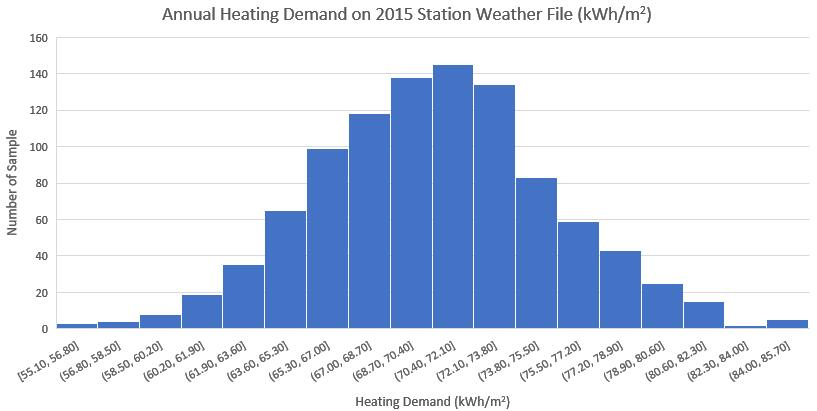
\includegraphics[scale=0.65]{Sumatra_2015Distribution.jpg}
		\caption{Office Building Heating Demand Histogram}
		\label{fig:Sumatra_StationHistogram}
		\end{figure}	

	    \begin{figure}[H]
		\centering
		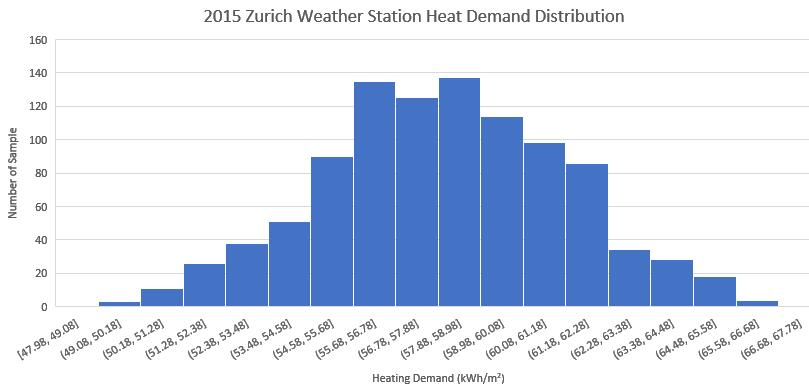
\includegraphics[scale=0.7]{Hongg_2015Distribution.jpg}
		\caption{Residential Building Heating Demand Histogram}
		\label{fig:Hongg_StationHistogram}
		\end{figure}

		Figure \ref{fig:Sumatra_Matrix} and Figure \ref{fig:Hongg_Matrix} show the correlation matrices for the office building and the residential building. Correlation matrix is a heat map with many pixels, where each pixel represent a correlation between two intersec parameters. A pixel with deep color indicates the correlation between two parameters is strong, while a pixel with light color indicates the correlation between two parameters is weak.\\
		
		In this thesis, the main focus is the correlation between heating demand, domestic hot water consumption and others. Therefore, the second last row represents the correlation between domestic hot water and other parameters, and the last row represents the correlation between heating demand and other parameters.\\
		
		The correlation matrix for the office building indicates that a strong correlation exists between office temperature setpoint (0.67)/solar absorptance (-0.34) and heating demand. Also, corridor temperature setpoint (0.28) and office appliance (-0.17) are the influential facters among all others. The residential building's correlation matrix also indicates that the key area setpoint temperature (0.58) and the solar absorptance (-0.45) are the influential facters to heating demand. In addition, air infiltration in residential building also showed a very strong correlation of 0.53, making it the second strongest correlated factor among all. As for domestic hot water, both correlation matrices showed that the domestic hot water demand is strongly depended on the domestic hot water demand of the key area.

		
	    \begin{figure}[H]
		\centering
		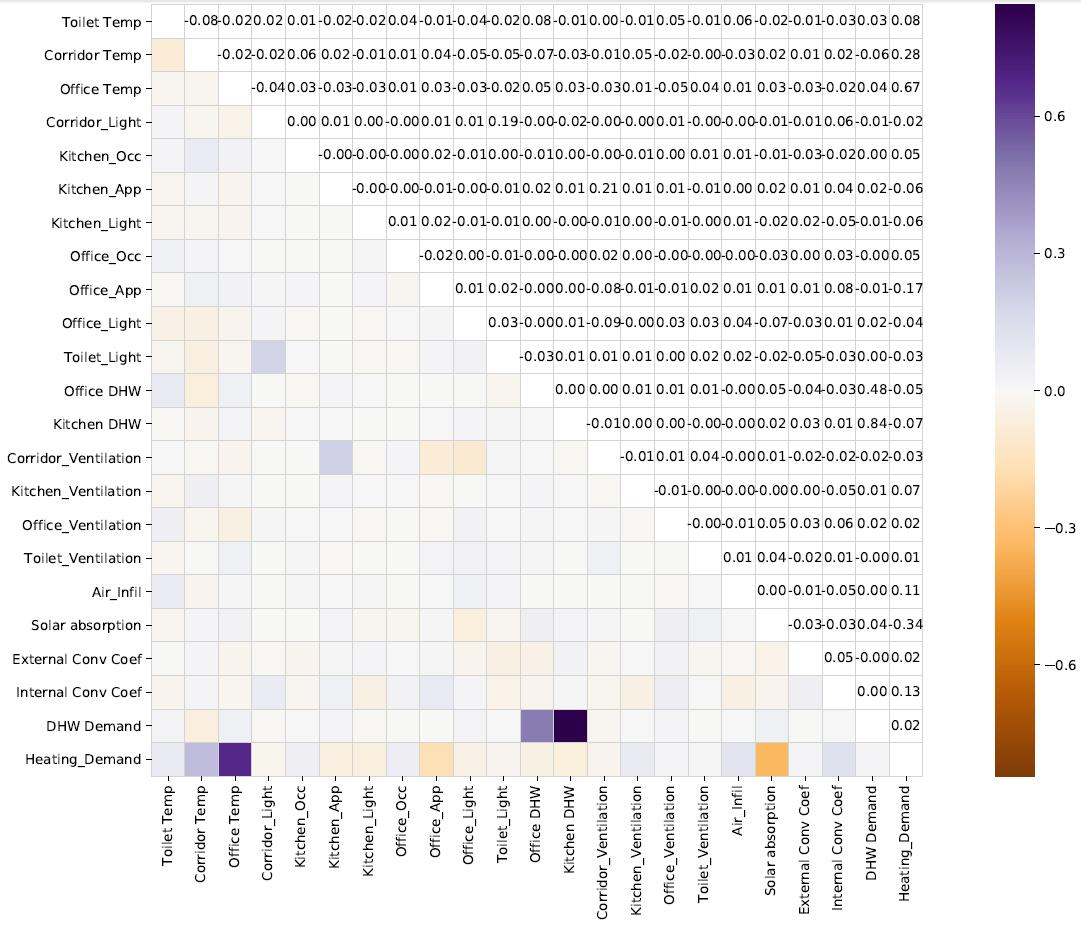
\includegraphics[scale=0.6]{Sumatra_Matrix.jpg}
		\caption{Office Building Correlation Matrix}
		\label{fig:Sumatra_Matrix}
		\end{figure}
			
	    \begin{figure}[H]
		\centering
		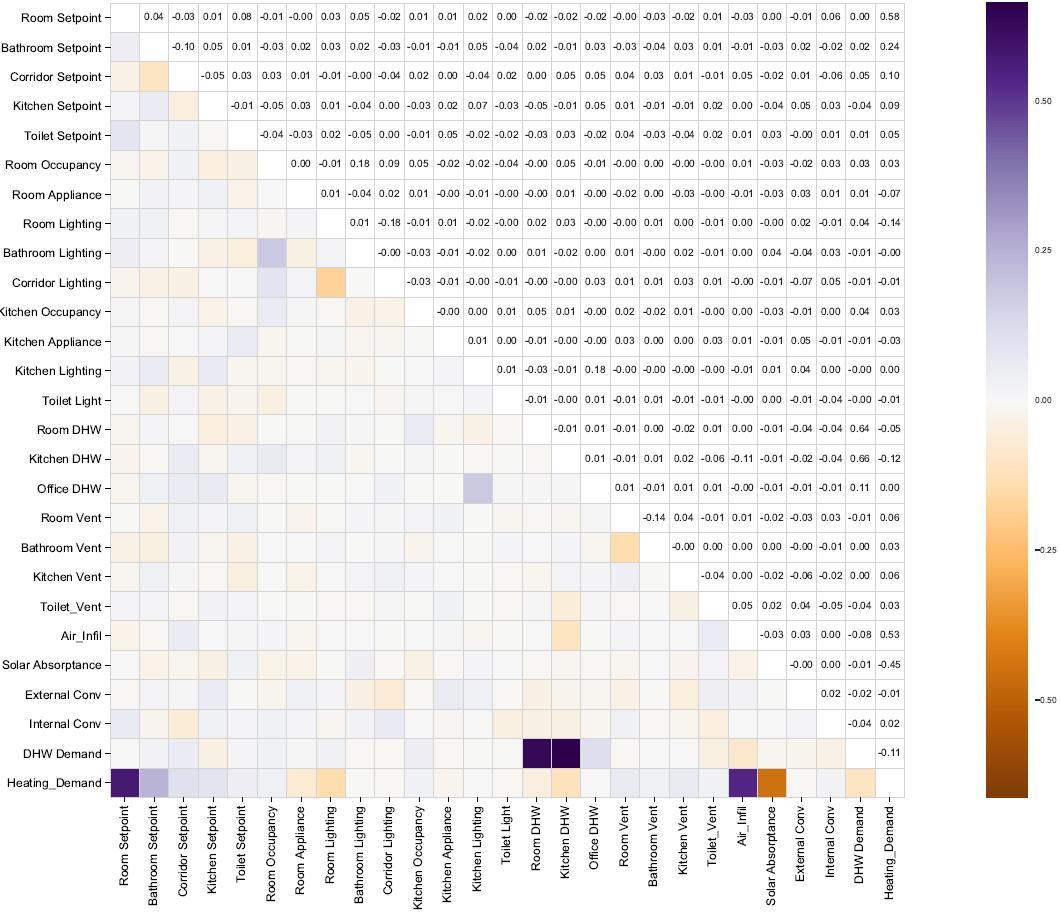
\includegraphics[scale=0.6]{Hongger_Matrix.jpg}
		\caption{Residential Building Correlation Matrix}
		\label{fig:Hongg_Matrix}
		\end{figure}


  	
    \section{Effect of Solar Absorptance on Heating Demand}
			In order to prove the influence of solar absorptance on heating demand, an extra set of 150 samples with different solar absorptance in the residential building are processed in jE-Plus and the results are displayed at Figure \ref{fig:Hong_solar} below.\\
			
    	    \begin{figure}[htbp]
    		\centering
    		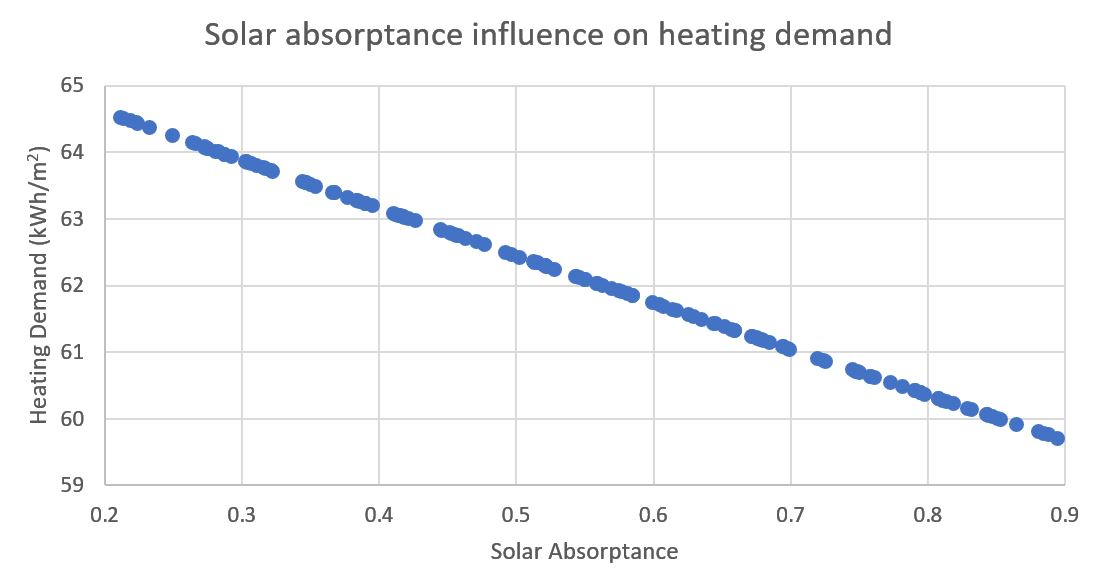
\includegraphics[scale=0.5]{Solar_HeatingDemand.JPG}
    		\caption{Influence of Solar Absorptance on Heating Demand (Residential Building)}
    		\label{fig:Hongg_solar}
    		\end{figure}			
        
        The results show that solar absorptance has proven its ability to influence the heating demand. By solely changing the solar absorptance, the heating demand can achieve a $\pm 4\%$ variation on the residential building. As $50\%$ of the 1000 parameter variation samples fall within the range of $\pm 3.4\%$ of average energy consumption (the residential building), it can conclude that solar absorptance in external facade is worth to be taken into account in energy calculations.

	\section{Effect of Convection Coefficient on Heating Demand}
        	As the correlation matrix above indicates a weak correlation between heating demand and heat convection coefficients, which is contradicted to the hypothesis that heat convection coefficient is an important factor in heating demand calculation, another set of simulation with 150 extra samples are processed. These simulations use the calibrated building model, with the only difference being the variations in convection coefficient (ranging from 90\% to 110\% of the calibrated values).The results shown in the Figure below indicate a $\pm 2\%$ variation on heating demand. Therefore, it is clear that $\pm 10\%$ of the heat convection coefficient would have less effects on heating demand than altering the solar absorptance from 0.2 to 0.9. \\ 
        	
          	\begin{figure}[htbp]
    		\centering
    		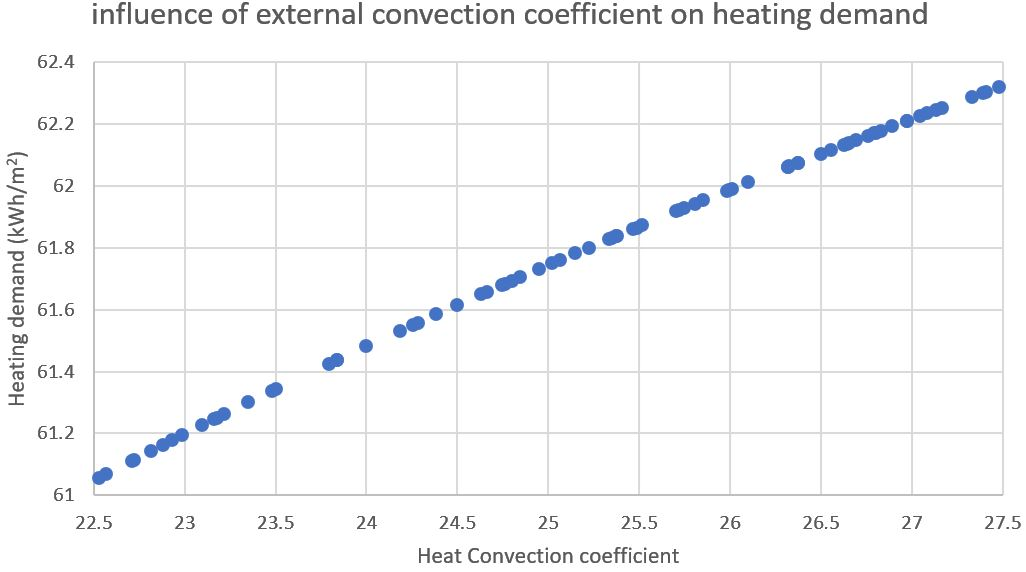
\includegraphics[scale=0.5]{Hongg_ConvCoe.JPG}
    		\caption{Influence of Heat Convection Coefficient on Heating Demand (Residential Building)}
    		\label{fig:Hongg_convcoef}
    		\end{figure}
        
        \subsection{Global Warming and Heat Island Effect}
		Figure \ref{fig:Sumatra_Comp} and \ref{fig:Hongg_Comp} shows the heating demand variation range under three different outdoor environments, namely, the SIA standard hourly data, the 2015 station weather, and the generated heat island weather based on the 2015 station weather. The annual heating demand range shows a clear decline as the average outdoor dry-bulb temperature gets higher.

	    \begin{figure}[H]
		\centering
		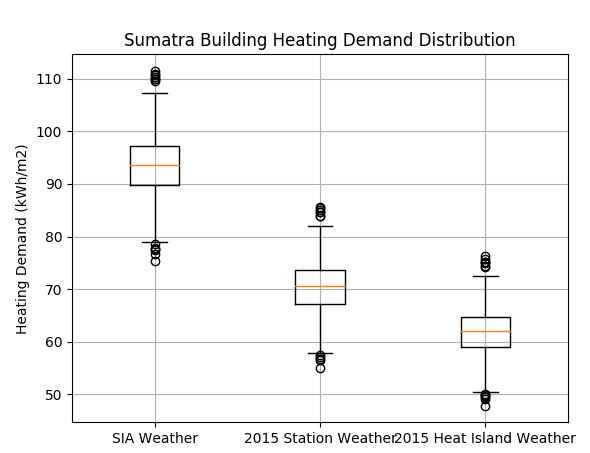
\includegraphics[scale=0.7]{Sumatra_Comparison.jpg}
		\caption{Office Building Annual Heating Demand Comparison with 3 Different Weather Files}
		\label{fig:Sumatra_Comp}
		\end{figure}

	    \begin{figure}[H]
		\centering
		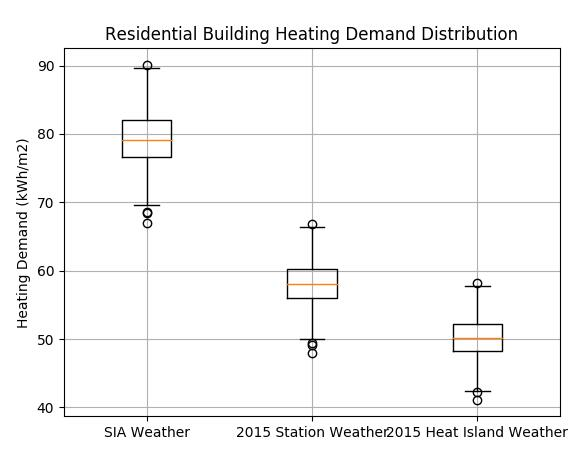
\includegraphics[scale=0.7]{Hongg_Comparison.jpg}
		\caption{Residential Building Annual Heating Demand Comparison with 3 Different Weather Files}
		\label{fig:Hongg_Comp}
		\end{figure}
		


\chapter{Discussion}
    From the calculation and simulation results of the previous chapter, there are a few points that worth mentioning. For static calculation, the SIA 380/1 standard calculatiom method can achieve a reasonably accurate result when an updated weather information is implemented. The standard can probably consider using internal (net) area instead of external (gross) area for energy calculation, as it provides a more accurate results when net area (excluding walls) is used in calculation.\\
    
    For dynamic simulation, weather information is also critical as varying the outdoor temperatuer can significantly change the resulting simulation heating demand. Also, a more accurate algorithm to simulate heat island effect is needed, as the temperature in city area can differ largely from the weather station's temperature even they are very close to each other. In addition, calibration process is important for analyzing the hourly building performance and gives more confidence in annual energy analyses.\\
    
    At the current stage, it is known that the performance gap come from a number of wrong assumptions of building parameters and schedules. However, these wrong assumptions managed to achieve an internal balance and the combination of these current standard assumptions can indeed provide a reasonably accurate results in macroscopic scale (annual per square meter demand for example). For example, an over estimated heat convection coefficient may lead to a higher energy demand, but an over estimated internal loads would lead to a lower energy demand, and the effect of both over estimation cancel each other. To obtain true accuracy, review or modification are needed for not only a single parameters but also all the others. Improving a single assumption without considering others would even lead to more diverse and inaccurate results.\\



\chapter{Conclusion}
    In conclusion, this thesis aims to reduce the deviation between calculated and measured heating demands and find the limitations and short-comings in SIA 380/1 calculation method. A residential building and an office building are accurately modeled and calculated using SIA 180 standard calculation method and EnergyPlus dynamic simulation engine. Both buildings are firstly calibrated until the indoor temperature profile is matched. Then, both buildings are subjected to a large number of simulations with different parameters. Finally, the most influential building simulation parameters are found out by processing the results using different graphic representations approaches such as correlation matrix, histogram and scatter plots. \\

    From the static calculation, the result shows that when applying net floor area and a more recent (2015) weather information from a nearby weather station in static calculation, the annual heating demand are macroscopically close to the measurement value. The results also indicates that the standard SIA 381/2 weather database provides information that is significantly different from the actual weather information in Zurich city. On average, the SIA 381/2 weather data is about 4 degrees lower than the recorded value in year 2015.\\

    From the dynamic calculation, the result shows that the origin simulation has a much lower energy consumption than the measured value. This is partly because of a wrong assumption on building air-tightness. In addition, the performance gap on annual heating demand closes when using a high external convection coefficient (SIA standard value of 25 W/m.K), which indicates an probability of over-estimated internal loads.\\

    The calibration processes have confirmed an over-estimation problem in internal loads, and discovered some previous unnoticed over-estimation problems in SIA 2024 lighting standards. The results indicates that the window blinds may be put down in summer for most of the time, and occupants are likely to open the window in un-heating period.\\

    Finally, the results from the building parameter variations indicate that the most influential parameters in simulation are key area temperature heating set points, external wall solar absorptance, infiltration and key area lighting schedules.\\

    Considering the above mentioned and discussed findings, in order to obtain higher simulation accuracy and reduce the performance gap, it is recommended to create an accurate building envelope, spend more effort on observing and recording the typical user behavior and occupancy patterns, apply accurate outdoor environment such as site dry-bulb temperature and wind speed, as well as using a set of more comprehensive and representative lighting and electronic schedule and activity assumptions.





% This displays the bibliography for all cited external documents. All references have to be defined in the file references.bib and can then be cited from within this document.
\bibliographystyle{IEEEtran}
\bibliography{references}

% This creates an appendix chapter, comment if not needed.
\appendix

\chapter{Assumptions}\label{sec:assumptions}

	The following assumptions are applied in constructing the building geometries and building envelopes in DesignBuilder \& EnergyPlus. All of the assumptions are for simplification of the modelling processes.\\ 

	\textit{Adiabatic Walls}\\
	As the residential building is attached to other buildings on both sides, the two walls that attach other buildings are seen as adiabatic. Similarily, as the north facade of the office building is attached to another building, it is also seen as adiabatic wall.\\

	\textit{No underground warehouses}\\
	The cellar of the residential building is not considered in this thesis and assume a constant temperature of 18 degree environment attach the ground floor.\\

	\textit{Ignore the tilted roof and loft}\\
	Due to lack of in about the internal layout of the top floor, the tilted roof and the loft of the residential building is represented as a regular size floor with exactly the same layout as the first floor.\\

	\textit{Ignore the vegitation covering}\\
	The majority part of the northen and the easten facade of the office building as well as both external walls of the residential building are covered with plants. However, as the effect of vegitation covering is unknow, the vegitation layer of these facade is ignored in the modeling and analysis process.\\


\chapter{TARP Method Calculation}\label{sec:tarp}
	The standard calculation SIA380/1 uses a fixed external heat convection coefficient of 25W/m$^2$K and an internal heat convection coefficient of 7.7W/m$^2$K regardless the internal \& external environment. However, many other research have purposed other methods to calculate the convection coefficient. One of the simple method that is used and supported by EnergyPlus is called \textit{TARP method}, which is taking the internal and external thermal condition as well as the surface roughness and air movement speed into account. The \textit{TRAP method} is given in the following fomular set below: \\

	\[h_c = h_f + h_n\]
	where $h_c$ is heat convection coefficient in W//m$^2$K

	\[h_f = 2.537 W_f R_f \left(\frac{PV_z}{A}\right)^\frac{1}{2}\]
	\[W_f = 1  \text{   for windward surface}\]
	\[W_f = 0.5 \text{   for leeward surface}\]

	\[R_f = 1.67 \text{: for brick surface}\]
	\[R_f = 1.52 \text{: for concrete surface}\]
	\[R_f = 1.13 \text{: for clear pine surface}\]
	\[R_f = 1 \text{: for glass surface}\]
	\[h_n = 1.31 | \Delta T|^{1/3} \text{: for vertical surface}\]
	

\chapter{Static Calculation Formulas and Results}\label{sec:siacalculation}
	In this thesis, The SIA380/1 calculation is performed as an excel sheet calculation. A detailed calculation information is given in the tables below, and a detail result breakdown of heat gain and losses is given in the results part.
	\section{Heat Losses}
	\textbf{Transmission Heat Loss}\\

		\[\dot{Q}_{transmission} =\frac{ A_{surface} \cdot U \cdot HDD \cdot 24 \cdot 3600}{A_{floor} \cdot 10^6}\]
		where:\\
		$\dot{Q}_{transmission}$: Heat transmission in $MJ/m^2$\\
		$A_{surface}$: Surface area of building element in $m^2$\\
		$U$: U-Value of building element in $ W/m^2K$\\
		$HDD$: Heating degree days\\
		$A_{floor}$: Total conditioned area of entire building\\

		The ground floor use a different formula to calculate the heat transmission heat loss.
		\[\dot{Q}_{\text{ground}} = \frac{ A_{c} \cdot U \cdot HT \cdot \Delta T \cdot 24 \cdot 3.6}{1000 \cdot A_{floor}}\]
		where:\\
		$A_c$: ground area (in m$^2$)\\
		$HT$: Heating days\\
		$U$: U-value of the element\\
		$\Delta T$: Temperature different between heating setpoint temperature and the unheated zone temperature\\

		The U-value of the building elements can be calculated by the formula below: \\
		\[U = \frac{1}{R_{Ex}+R_{Layer}+R_{In}} = \frac{1}{\frac{1}{h_{ex}}+\sum_{i}\frac{d_i}{\lambda_i} + \frac{1}{h_{in}}}\]
		where:\\
		$h_{ex}$: External heat convection coefficient in $W/m^K$\\
		$h_{in}$: Internal heat convection coefficient\\
		$R_{Layer}$: Total heat resistance of building element in $m^K/W$\\
		$d$: thickness of building element in $m$\\
		$\lambda$: Thermal conductivity of building element in $W/mK$\\


	\textbf{Thermal Bridge Heat Loss}\\
		The loss through thermal bridges can be calculated in the following formula.\\
		\[\dot{Q}_{TB} = \frac{\Psi \cdot L \cdot HDD \cdot 24 \cdot 3600}{A_{floor} \cdot 10^6}\]
		where:\\
		$\dot{Q}_{TB}$: Thermal bridge heat loss in $MJ/m^2$\\
		$L$: Length of thermal bridge\\
		$\Psi$: Thermal bridge loss factor\\ 
		$HDD$: Heating degree days\\
		$A_{floor}$: Total conditioned area of entire building\\


	\textbf{Ventilation Loss}\\
		The ventilation heat loss is given below:\\
		\[Q_{\text{vent}} = \frac{\dot{V} \cdot c_{p,air} \cdot HDD}{24 \cdot 1000}\]
		where:\\
		$\dot{Q}_{\text{vent}}$: Ventilation heat loss in $MJ/m^2$\\
		$\dot{V} = 0.7$: Ventilation rate in $m^3/m^2\cdot h$\\
		$c_{p,air} = 1.16$: Heat capacity of air $kJ/m^3 \cdot K$\\
		$HDD$: heating degree days\\
	
	\textbf{Total Heat Loss}\\
	The total heat loss is the sum of the individual heat losses.
	\[\text{Total Heat Loss = Transmission Heat Loss + Thermal Bridge Heat Loss + Ventilation Loss}\]

	\section{Heat Gains}
	\textbf{Solar Gains}\\
	The heat gain from solar energy is given below: \\
	\[Q_{\text{solar}} = \frac{G \cdot A_{\text{glazing}} \cdot f_1 \cdot f_2 \cdot f_3 \cdot f_g \cdot g}{A_{floor}} \]

	where:\\
	$f_1$, $f_2$, $f_3$, $f_g$: Reduction factors for shading, frames, overhangs, and impurities on the window, the values are given in previous calculations\\
	$g$: g-value of the window, transmittance\\
	$G$: Unit solar radiation onto the surface in $MJ/m^2$\\
	$A_{\text{glazing}}$: Window area in $m^2$\\

	
	\textbf{Internal Gains by electronics}\\
	The heat gain from electronics comes from a factor of electricity demand.
	\[\dot{Q}_{\text{elec}} = \frac{E_{unit}  \cdot f_{ele} \cdot HT \cdot 3.6}{365} \]
	$\dot{Q}_{\text{elec}}$: Heat gain by electronics in MJ/m$^2$\\
	$E_{unit}$: Unit area electricity demand in $kWh/m^2$\\
	$f_{ele} = 0.7$: electricity gain factor\\
	$HT$: Heating day\\
	$A_{floor}$: Total floor area\\


	\textbf{Internal Gains by person}\\
	The internal gain from occupant activities is given below:\\

	\[Q_{\text{occ}} = \frac{\dot{q}_{pl} \cdot h_{\text{present}} \cdot 365 \cdot 3.6}{\text{Occ} \cdot  1000}\]
	where:\\
	$\dot{Q}_{\text{occ}}$: Internal gains by person in MJ/m$^2$\\
	$\text{Occ}$: Unit area occupancy, Occ = 40$m^2/pl$ for residential, 20$m^2/pl$ for office building\\
	$\dot{q}_{pl} = 70W/pl$: internal gain produce by a single person\\
	$h_{\text{present}}$: present hour per day, 12 for residential building, 6 for office building\\



	\textbf{Total Heat Gain}\\
	\[Q_{\text{gain}} = (Q_{\text{solar}} + Q_{\text{elec}} + Q_{\text{occ}}) \cdot x\]
	where x is heat gain factor given by:
	\[ x = \frac{\sum \text{Heat Gain}}{\sum \text{Heat Loss}}\]

	\section{Total Heating Demand}
	The total heating demand is given by:
	\[\text{Total Heating Demand = Total Heat Loss - Total Heat Gain}\]

	\newpage 
	\section{Residential Building Heating Demand Breakdown}		
		\textbf{Transmission Heat Loss}\\
		Table \ref{tab:HonggTransmission} below show a the transmission heat loss for each building element under both SIA 381/2 weather data and the 2015 weather station data. The unit of heat loss is in MJ/m$^2$.
				% Table generated by Excel2LaTeX from sheet 'Sheet1'
		\begin{table}[htbp]
		\small
		\centering
		\caption{Heat Transmission Heat Loss of Residential Building}
		    \begin{tabular}{|ccccc|}
		    \toprule
		    \multicolumn{5}{|c|}{\textbf{Heat Transmission Loss}} \\
		    \midrule
		          & \multicolumn{1}{p{4.785em}}{Area m2} & \multicolumn{1}{p{4.785em}}{U-Value W/m2.K} & \multicolumn{1}{p{5.715em}}{Loss (SIA) MJ/m2} & \multicolumn{1}{p{5.715em}|}{Loss(2015) MJ/m2} \\
		    \midrule
		    Outside Wall & 208.6088 & 1.006 & 152.60 & 117.63 \\
		    Window FE-EG-1a & 9.9   & 2.379 & 17.13 & 13.21 \\
		    Window FE-EG-2a & 26    & 2.388 & 45.16 & 34.82 \\
		    Window FE-EG-3a & 3     & 2.19  & 4.78  & 3.68 \\
		    Window FE-EG-4a & 20.8  & 2.285 & 34.57 & 26.65 \\
		    Window FE-TH-1a & 3.7   & 2.33  & 6.27  & 4.83 \\
		    Door Tur-TH & 2.5   & 3.5   & 6.36  & 4.91 \\
		    Ceiling & 101.2115 & 1.6145418 & 37.92 & 31.90 \\
		    Ground floor & 101.2115 & 1.3504216 & 31.72 & 26.69 \\
		    \midrule
		    Total &       &       & 336.52 & 264.32 \\
		    \bottomrule
		    \end{tabular}%
		  \label{tab:HonggTransmission}%
		\end{table}%

		\textbf{Ventilation Heat Loss}\\
		Table \ref{tab:HonggVentLoss380} below shows the monthly and the annual ventilation heat loss per $m^2$ of floor area under monthly SIA 382/1 weather data and 2015 Zurich weather station data. Similarly, the energy loss is in MJ/m$^2$.\\
		% Table generated by Excel2LaTeX from sheet 'Sheet1'
		\begin{table}[H]
		\centering
		\small
		\caption{Residential Building Ventilation Heat Loss}
		    \begin{tabular}{|p{6.855em}ccccccccccccc|}
		    \toprule
		    \multicolumn{14}{|c|}{Ventilation Heat Loss MJ/m2} \\
		    \midrule
		    \multicolumn{1}{|c}{Month} & Jan  & Feb  & Mar  & Apr  & May  & Jun  & Jul  & Aug  & Sep  & Oct  & Nov  & Dec  & Sum \\
		    \midrule
		    Heating Degree Days (2015) & 498  & 519  & 344  & 149  & 30.6 & 0    & 0    & 0    & 17.8 & 225  & 268  & 462  & 2513 \\
		    Heating Degree Days (SIA) & 615  & 501  & 467  & 255  & 110  & 23   & 7    & 6    & 35   & 207  & 433  & 601  & 3260 \\
		    Ventilation Loss SIA & 12   & 9.76 & 9.1  & 4.97 & 2.14 & 0.45 & 0.14 & 0.12 & 0.68 & 4.03 & 8.44 & 11.7 & 63.53 \\
		    Ventilation Heat loss 2015 & 9.71 & 10.1 & 6.7  & 2.9  & 0.6  & 0    & 0    & 0    & 0.35 & 4.38 & 5.23 & 9    & 48.98 \\
		    \bottomrule
		    \end{tabular}%

		  \label{tab:HonggVentLoss380}%
		\end{table}%

		\textbf{Heat Loss Through Thermal Bridge}\\
		The heat loss through thermal bridge of all building elements are shown below in Table \ref{tab:HonggerThermalBridge} below.
		\begin{table}[H]
		\small
		\centering
		\caption{Thermal Bridge Calculation For Residential Building}
		    \begin{tabular}{ccrccccc}
		    \toprule
		    \multicolumn{1}{l}{Nr.} & \multicolumn{2}{c}{Component} & Lost Coefficient & Length & H(U*A*b) & SIA 381/2 & 2015 Zurich \\
		         &      &      & W/mK & m    & W/K  & MJ/m2 & MJ/m2 \\
		    \midrule
		    1    & \multicolumn{1}{r}{Tur-TH} & \multicolumn{1}{l}{(Sturz)} & 0.1  & 1    & 0.1  & 0.07323747 & 0.056459083 \\
		    2    & \multicolumn{1}{r}{Tur-TH} & \multicolumn{1}{l}{(Brustung)} & 0.1  & 1    & 0.1  & 0.07323747 & 0.056459083 \\
		    3    & \multicolumn{1}{r}{Tur-TH} & \multicolumn{1}{l}{(Leibung)} & 0.1  & 5    & 0.5  & 0.36618737 & 0.282295415 \\
		    4    & \multicolumn{1}{r}{FE-EG-1a} & \multicolumn{1}{l}{(Sturz)} & 0.1  & 3.6  & 0.36 & 0.26365491 & 0.203252699 \\
		    5    & \multicolumn{1}{r}{FE-EG-1a} & \multicolumn{1}{l}{(Brustung)} & 0.1  & 3.6  & 0.36 & 0.26365491 & 0.203252699 \\
		    6    & \multicolumn{1}{r}{FE-EG-1a} & \multicolumn{1}{l}{(Leibung)} & 0.1  & 5.8  & 0.58 & 0.42477735 & 0.327462681 \\
		    7    & \multicolumn{1}{r}{FE-EG-2a} & \multicolumn{1}{l}{(Sturz)} & 0.1  & 10   & 1    & 0.73237474 & 0.56459083 \\
		    8    & \multicolumn{1}{r}{FE-EG-2a} & \multicolumn{1}{l}{(Brustung)} & 0.1  & 10   & 1    & 0.73237474 & 0.56459083 \\
		    9    & \multicolumn{1}{r}{FE-EG-2a} & \multicolumn{1}{l}{(Leibung)} & 0.1  & 52   & 5.2  & 3.80834863 & 2.935872315 \\
		    10   & \multicolumn{1}{r}{FE-EG-3a} & \multicolumn{1}{l}{(Sturz)} & 0.1  & 2.5  & 0.25 & 0.18309368 & 0.141147707 \\
		    11   & \multicolumn{1}{r}{FE-EG-3a} & \multicolumn{1}{l}{(Brustung)} & 0.1  & 2.5  & 0.25 & 0.18309368 & 0.141147707 \\
		    12   & \multicolumn{1}{r}{FE-EG-3a} & \multicolumn{1}{l}{(Leibung)} & 0.1  & 12   & 1.2  & 0.87884968 & 0.677508996 \\
		    13   & \multicolumn{1}{r}{FE-EG-4a} & \multicolumn{1}{l}{(Sturz)} & 0.1  & 13   & 1.3  & 0.95208716 & 0.733968079 \\
		    14   & \multicolumn{1}{r}{FE-EG-4a} & \multicolumn{1}{l}{(Brustung)} & 0.1  & 13   & 1.3  & 0.95208716 & 0.733968079 \\
		    15   & \multicolumn{1}{r}{FE-EG-4a} & \multicolumn{1}{l}{(Leibung)} & 0.1  & 41.6 & 4.16 & 3.0466789 & 2.348697852 \\
		    16   & \multicolumn{1}{r}{FE-TH-1a} & \multicolumn{1}{l}{(Sturz)} & 0.1  & 3.68 & 0.37 & 0.27097865 & 0.208898607 \\
		    17   & \multicolumn{1}{r}{FE-TH-1a} & \multicolumn{1}{l}{(Brustung)} & 0.1  & 3.68 & 0.37 & 0.27097865 & 0.208898607 \\
		    18   & \multicolumn{1}{r}{FE-TH-1a} & \multicolumn{1}{l}{(Leibung)} & 0.1  & 7.8  & 0.78 & 0.57125229 & 0.440380847 \\
		    \midrule
		    \multicolumn{3}{c}{Total} &     & 191.8 &            & 14.05 & 10.83 \\
		    \bottomrule
		    \end{tabular}%
		  \label{tab:HonggerThermalBridge}%
		\end{table}%

		\textbf{Internal Gains by Occupants}\\ 
		% Table generated by Excel2LaTeX from sheet 'Sheet1'
		\begin{table}[htbp]
		\centering
		\caption{Internal Gains by Occupants in Residential Building}
		    \begin{tabular}{cccc}
		    \toprule
		    \multicolumn{4}{c}{Internal Gains by person} \\
		    \midrule
		    \multicolumn{1}{p{8.07em}}{Occupancy m2/P} & \multicolumn{1}{p{7em}}{Unit Gain W/P} & \multicolumn{1}{p{7.355em}}{Present hour } & \multicolumn{1}{p{7.355em}}{Gain (MJ/m2)} \\
		    40    & 70    & 12    & 27.594 \\
		    \bottomrule
		    \end{tabular}%
		  \label{tab:HonggOccupancyGain}%
		\end{table}%

		\textbf{Internal Gains by Electronics}\\
		\begin{table}[htbp]
		\centering
		\caption{Heat Gain by Electronics in Residential Building}
		    \begin{tabular}{ccccc}
		    \toprule
		    \multicolumn{5}{c}{Internal Gains by electronics} \\
		    \midrule
		    \multicolumn{1}{p{5.355em}}{Weather data} & \multicolumn{1}{p{5.355em}}{Unit demand (kWh/m2)} & \multicolumn{1}{p{5.355em}}{Factor} & \multicolumn{1}{p{5.355em}}{Heating Day} & \multicolumn{1}{p{5.355em}}{Heat Gain (MJ/m2)} \\
		    2015  & 28    & 0.7   & 175   & 33.83 \\
		    SIA   & 28    & 0.7   & 208   & 40.21 \\
		    \bottomrule
		    \end{tabular}%
		  \label{tab:HonggElecGain}%
		\end{table}%

		\textbf{Internal Gains by Solar Radiation}\\
		\begin{table}[htbp]
		\centering
		\small
		\caption{Solar Gains in Residential Building}
		    \begin{tabular}{lrrrrrrrrrrr}
		    \toprule
		    \multicolumn{12}{c}{Solar Gains ($MJ/m^2$)} \\
		    \midrule
		    \multicolumn{1}{p{4.215em}}{Window Names} & \multicolumn{1}{c}{Orient} & \multicolumn{1}{c}{Area} & \multicolumn{1}{c}{f1} & \multicolumn{1}{c}{f2} & \multicolumn{1}{c}{f3} & \multicolumn{1}{c}{fg} & \multicolumn{1}{c}{g} & \multicolumn{1}{p{4.57em}}{Radiation\newline{}SIA} & \multicolumn{1}{p{4.57em}}{Radiation\newline{}2015} & \multicolumn{1}{p{3.8em}}{Solar Gain (SIA)} & \multicolumn{1}{p{3.8em}}{Solar Gain (2015)} \\
		    \midrule
		    FE-EG-1a & \multicolumn{1}{l}{NE} & 6.9   & 0.89  & 0.97  & 0.99  & 0.64  & 0.5   & 1563.92 & 1388.59 & 7.62  & 6.77 \\
		    FE-EG-2a & \multicolumn{1}{l}{NE} & 10.4  & 0.89  & 0.97  & 0.99  & 0.53  & 0.5   & 1563.92 & 1388.59 & 9.51  & 8.45 \\
		    FE-EG-2a & \multicolumn{1}{l}{SW} & 15.6  & 0.82  & 0.97  & 0.98  & 0.53  & 0.5   & 2653.31 & 2683.81 & 22.08 & 22.34 \\
		    FE-EG-3a & \multicolumn{1}{l}{SW} & 3     & 0.82  & 0.97  & 0.98  & 0.3   & 0.5   & 2653.31 & 2683.81 & 2.40  & 2.43 \\
		    FE-EG-4a & \multicolumn{1}{l}{NE} & 14.4  & 0.89  & 0.97  & 0.99  & 0.5   & 0.5   & 1563.92 & 1388.59 & 12.43 & 11.03 \\
		    FE-EG-4a & \multicolumn{1}{l}{SW} & 6.4   & 0.82  & 0.97  & 0.98  & 0.5   & 0.5   & 2653.31 & 2683.81 & 8.55  & 8.64 \\
		    FE-TH-1a & \multicolumn{1}{l}{NE} & 2.88  & 0.89  & 0.97  & 0.99  & 0.54  & 0.5   & 1563.92 & 1388.59 & 2.68  & 2.38 \\
		    FE-TH-1a & \multicolumn{1}{l}{SW} & 2.8   & 0.82  & 0.97  & 0.98  & 0.54  & 0.5   & 2653.31 & 2683.81 & 4.04  & 4.08 \\
		    \midrule
		    Total &       &       &       &       &       &       &       &       &       & 69.32 & 66.13 \\
		    \bottomrule
		    \end{tabular}%
		  \label{tab:HonggSolarGain}%
		\end{table}%

		\newpage 
		\section{Office Building Heating Demand Breakdown}

		\textbf{Transmission Heat Loss}\\
		% Table generated by Excel2LaTeX from sheet 'Sheet1'
		\begin{table}[H]
		\centering
		\caption{Transmission Heat Loss of Office Building}
		    \begin{tabular}{crrrr}
		    \toprule
		    \multicolumn{5}{c}{Heat Transmission Loss $MJ/m^2$} \\
		    \midrule
		          & \multicolumn{1}{p{4.215em}}{Area} & \multicolumn{1}{p{4.215em}}{U-Value} & \multicolumn{1}{p{4.215em}}{Loss \newline{}(SIA) } & \multicolumn{1}{p{4.215em}}{Loss (2015)} \\
		    \midrule
		    Earth Wall East & \multicolumn{1}{c}{121.73} & \multicolumn{1}{c}{3.47} & \multicolumn{1}{c}{143.92} & \multicolumn{1}{c}{110.94} \\
		    External Wall East & \multicolumn{1}{c}{110.34} & \multicolumn{1}{c}{0.96} & \multicolumn{1}{c}{36.16} & \multicolumn{1}{c}{27.88} \\
		    Outside Wall Other & \multicolumn{1}{c}{159.35} & \multicolumn{1}{c}{1.37} & \multicolumn{1}{c}{74.43} & \multicolumn{1}{c}{57.38} \\
		    Window FE1 & \multicolumn{1}{c}{198.00} & \multicolumn{1}{c}{2.00} & \multicolumn{1}{c}{134.98} & \multicolumn{1}{c}{104.05} \\
		    Window FE2 & \multicolumn{1}{c}{8.13} & \multicolumn{1}{c}{2.50} & \multicolumn{1}{c}{6.92} & \multicolumn{1}{c}{5.33} \\
		    Window FE3 & \multicolumn{1}{c}{2.70} & \multicolumn{1}{c}{2.50} & \multicolumn{1}{c}{2.30} & \multicolumn{1}{c}{1.77} \\
		    Window FE4 & \multicolumn{1}{c}{10.50} & \multicolumn{1}{c}{2.05} & \multicolumn{1}{c}{7.32} & \multicolumn{1}{c}{5.65} \\
		    Window FE5 & \multicolumn{1}{c}{7.79} & \multicolumn{1}{c}{2.07} & \multicolumn{1}{c}{5.50} & \multicolumn{1}{c}{4.24} \\
		    Window FE6 & \multicolumn{1}{c}{4.50} & \multicolumn{1}{c}{2.03} & \multicolumn{1}{c}{3.11} & \multicolumn{1}{c}{2.40} \\
		    Window FE7 & \multicolumn{1}{c}{5.76} & \multicolumn{1}{c}{2.04} & \multicolumn{1}{c}{4.01} & \multicolumn{1}{c}{3.09} \\
		    Window FE8 & \multicolumn{1}{c}{2.93} & \multicolumn{1}{c}{1.91} & \multicolumn{1}{c}{1.90} & \multicolumn{1}{c}{1.47} \\
		    Ceiling & \multicolumn{1}{c}{231.96} & \multicolumn{1}{c}{0.88} & \multicolumn{1}{c}{69.39} & \multicolumn{1}{c}{53.49} \\
		    Ground floor & \multicolumn{1}{c}{231.96} & \multicolumn{1}{c}{1.90} & \multicolumn{1}{c}{38.32} & \multicolumn{1}{c}{32.24} \\
		    \midrule
		    Total &       &       & 528.26 & 409.92 \\
		    \bottomrule
		    \end{tabular}%
		  \label{tab:SumatraTransmission Loss}%
		\end{table}%


		\textbf{Ventilation Heat Loss}\\
% Table generated by Excel2LaTeX from sheet 'Sheet1'
\begin{table}[H]
  \centering
  \small
  \caption{Ventilation Heat Loss of Office Building}
    \begin{tabular}{|p{4.5em}rrrrrrrrrrrrr|}
    \toprule
    \multicolumn{14}{|c|}{Ventilation Heat Loss (MJ/m2)} \\
    \midrule
    \multicolumn{1}{|l}{ } & \multicolumn{1}{l}{Jan} & \multicolumn{1}{l}{Feb} & \multicolumn{1}{l}{Mar} & \multicolumn{1}{l}{Apr} & \multicolumn{1}{l}{May} & \multicolumn{1}{l}{Jun} & \multicolumn{1}{l}{Jul} & \multicolumn{1}{l}{Aug} & \multicolumn{1}{l}{Sep} & \multicolumn{1}{l}{Oct} & \multicolumn{1}{l}{Nov} & \multicolumn{1}{l}{Dec} & \multicolumn{1}{l|}{Sum} \\
    \midrule
    \multicolumn{1}{|l}{HDD 2015} & 498.3 & 518.9 & 343.8 & 148.6 & 30.6 & 0.0  & 0.0  & 0.0  & 17.8 & 224.9 & 268.3 & 461.9 & 2513.15 \\
    \multicolumn{1}{|l}{HDD SIA} & 615.0 & 501.0 & 467.0 & 255.0 & 110.0 & 23.0 & 7.0  & 6.0  & 35.0 & 207.0 & 433.0 & 601.0 & 3260.00 \\
    Ventilation Loss 2015 & 9.71 & 10.11 & 6.70 & 2.90 & 0.60 & 0.00 & 0.00 & 0.00 & 0.35 & 4.38 & 5.23 & 9.00 & 48.98 \\
    Ventilation Loss SIA & 11.99 & 9.76 & 9.10 & 4.97 & 2.14 & 0.45 & 0.14 & 0.12 & 0.68 & 4.03 & 8.44 & 11.71 & 63.53 \\
    \bottomrule
    \end{tabular}%
  \label{tab:SumatraVentLoss}%
\end{table}%


		\textbf{Heat Loss Through Thermal Bridge}\\

% Table generated by Excel2LaTeX from sheet 'Sheet2'
\begin{table}[H]
\centering
\small
\caption{Thermal Bridge Heat Loss in Office Building}
    \begin{tabular}{ccccrrr}
    \toprule
    \multicolumn{7}{c}{Thermal Bridge Loss in Office Building ($MJ/m^2$)} \\
    \hline
    \multicolumn{3}{c}{Code} & \multicolumn{1}{p{2.785em}}{$\Psi$} & \multicolumn{1}{c}{Length\newline{} m} & \multicolumn{1}{p{3em}}{Loss (SIA)} & \multicolumn{1}{p{3em}}{Loss (2015)} \\
    \multicolumn{1}{l}{FE} & \multicolumn{1}{r}{1} & \multicolumn{1}{l}{(Sturz)} & \multicolumn{1}{r}{0.5} & 99   & 16.864 & 11.772 \\
    \multicolumn{1}{l}{FE} & \multicolumn{1}{r}{1} & \multicolumn{1}{l}{(Brustung)} & \multicolumn{1}{r}{0.5} & 99   & 16.864 & 11.772 \\
    \multicolumn{1}{l}{FE} & \multicolumn{1}{r}{1} & \multicolumn{1}{l}{(Leibung)} & \multicolumn{1}{r}{0.5} & 132  & 22.486 & 15.696 \\
    \multicolumn{1}{l}{FE} & \multicolumn{1}{r}{2} & \multicolumn{1}{l}{(Sturz)} & \multicolumn{1}{r}{0.5} & 3    & 0.511 & 0.357 \\
    \multicolumn{1}{l}{FE} & \multicolumn{1}{r}{2} & \multicolumn{1}{l}{(Brustung)} & \multicolumn{1}{r}{0.5} & 3    & 0.511 & 0.357 \\
    \multicolumn{1}{l}{FE} & \multicolumn{1}{r}{2} & \multicolumn{1}{l}{(Leibung)} & \multicolumn{1}{r}{0.5} & 5.4  & 0.920 & 0.642 \\
    \multicolumn{1}{l}{FE} & \multicolumn{1}{r}{3} & \multicolumn{1}{l}{(Sturz)} & \multicolumn{1}{r}{0.5} & 1.35 & 0.230 & 0.161 \\
    \multicolumn{1}{l}{FE} & \multicolumn{1}{r}{3} & \multicolumn{1}{l}{(Brustung)} & \multicolumn{1}{r}{0.5} & 1.35 & 0.230 & 0.161 \\
    \multicolumn{1}{l}{FE} & \multicolumn{1}{r}{3} & \multicolumn{1}{l}{(Leibung)} & \multicolumn{1}{r}{0.5} & 4    & 0.681 & 0.476 \\
    \multicolumn{1}{l}{FE} & \multicolumn{1}{r}{4} & \multicolumn{1}{l}{(Sturz)} & \multicolumn{1}{r}{0.5} & 5.1  & 0.869 & 0.606 \\
    \multicolumn{1}{l}{FE} & \multicolumn{1}{r}{4} & \multicolumn{1}{l}{(Brustung)} & \multicolumn{1}{r}{0.5} & 5.1  & 0.869 & 0.606 \\
    \multicolumn{1}{l}{FE} & \multicolumn{1}{r}{4} & \multicolumn{1}{l}{(Leibung)} & \multicolumn{1}{r}{0.5} & 12   & 2.044 & 1.427 \\
    \multicolumn{1}{l}{FE} & \multicolumn{1}{r}{5} & \multicolumn{1}{l}{(Sturz)} & \multicolumn{1}{r}{0.5} & 3.9  & 0.664 & 0.464 \\
    \multicolumn{1}{l}{FE} & \multicolumn{1}{r}{5} & \multicolumn{1}{l}{(Brustung)} & \multicolumn{1}{r}{0.5} & 3.9  & 0.664 & 0.464 \\
    \multicolumn{1}{l}{FE} & \multicolumn{1}{r}{5} & \multicolumn{1}{l}{(Leibung)} & \multicolumn{1}{r}{0.5} & 12   & 2.044 & 1.427 \\
    \multicolumn{1}{l}{FE} & \multicolumn{1}{r}{6} & \multicolumn{1}{l}{(Sturz)} & \multicolumn{1}{r}{0.5} & 3    & 0.511 & 0.357 \\
    \multicolumn{1}{l}{FE} & \multicolumn{1}{r}{6} & \multicolumn{1}{l}{(Brustung)} & \multicolumn{1}{r}{0.5} & 3    & 0.511 & 0.357 \\
    \multicolumn{1}{l}{FE} & \multicolumn{1}{r}{6} & \multicolumn{1}{l}{(Leibung)} & \multicolumn{1}{r}{0.5} & 6    & 1.022 & 0.713 \\
    \multicolumn{1}{l}{FE} & \multicolumn{1}{r}{7} & \multicolumn{1}{l}{(Sturz)} & \multicolumn{1}{r}{0.5} & 3.2  & 0.545 & 0.381 \\
    \multicolumn{1}{l}{FE} & \multicolumn{1}{r}{7} & \multicolumn{1}{l}{(Brustung)} & \multicolumn{1}{r}{0.5} & 3.2  & 0.545 & 0.381 \\
    \multicolumn{1}{l}{FE} & \multicolumn{1}{r}{7} & \multicolumn{1}{l}{(Leibung)} & \multicolumn{1}{r}{0.5} & 7.2  & 1.226 & 0.856 \\
    \multicolumn{1}{l}{FE} & \multicolumn{1}{r}{8} & \multicolumn{1}{l}{(Sturz)} & \multicolumn{1}{r}{0.5} & 3.9  & 0.664 & 0.464 \\
    \multicolumn{1}{l}{FE} & \multicolumn{1}{r}{8} & \multicolumn{1}{l}{(Brustung)} & \multicolumn{1}{r}{0.5} & 3.9  & 0.664 & 0.464 \\
    \multicolumn{1}{l}{FE} & \multicolumn{1}{r}{8} & \multicolumn{1}{l}{(Leibung)} & \multicolumn{1}{r}{0.5} & 4.5  & 0.767 & 0.535 \\
    \hline
    \multicolumn{4}{c}{Total} & 428  & 72.908 & 50.894 \\
    \bottomrule
    \end{tabular}%
  \label{tab:SumatraThermalBridgeLoss}%
\end{table}%

		\textbf{Internal Gains by Occupants}\\ 
% Table generated by Excel2LaTeX from sheet 'Sheet1'
\begin{table}[H]
  \centering
\caption{Internal Gains by Occupants in Office Building}
    \begin{tabular}{cccc}
    \toprule
    \multicolumn{4}{c}{Internal Gains by person} \\
    \midrule
    \multicolumn{1}{c}{Occupancy m2/P} & \multicolumn{1}{c}{Unit Gain W/P} & \multicolumn{1}{c}{Present hour (per day)} & \multicolumn{1}{c}{Gain (MJ/m2)} \\
    \midrule
    20   & 80   & 6    & 31.536 \\
    \bottomrule
    \end{tabular}%
  \label{tab:SumatraPersonGain}%
\end{table}%


		\textbf{Internal Gains by Electronics}\\
% Table generated by Excel2LaTeX from sheet 'Sheet1'
		\begin{table}[H]
		\centering
		\caption{Internal Gains by Electronics}
		    \begin{tabular}{lllll}
		    \toprule
		    \multicolumn{5}{p{30.135em}}{Internal Gains by electronics} \\
		    \midrule
		    \multicolumn{1}{p{5.215em}}{Weather Data} & \multicolumn{1}{p{6.355em}}{Unit Demand\newline{}(MJ/m2)} & \multicolumn{1}{p{5.855em}}{Factor} & \multicolumn{1}{p{6.355em}}{HT\newline{}(heating day)} & \multicolumn{1}{p{6.355em}}{Heat Gain\newline{}(MJ/m2)} \\
		    \midrule
		    \multicolumn{1}{p{5.215em}}{SIA} & 8    & 0.9  & 175  & 3.45 \\
		    2015 & 8    & 0.9  & 208  & 4.10 \\
		    \bottomrule
		    \end{tabular}%
		  \label{tab:SumatraElecGains}%
		\end{table}%



		\textbf{Internal Gains by Solar Radiation}\\

		\begin{table}[H]
		\centering
		\caption{Solar Gains in Office Building}
		    \begin{tabular}{llllllllllll}
		    \toprule
		    \multicolumn{12}{c}{Heat Gains through windows} \\
		    \midrule
		    \multicolumn{1}{p{3em}}{Window\newline{}Names} & Orient & \multicolumn{1}{p{2.5em}}{Area\newline{}m2} & f1   & f2   & f3   & fg   & g    & \multicolumn{1}{p{3em}}{Radiation\newline{}SIA} & \multicolumn{1}{p{3em}}{Radiation\newline{}2015} & \multicolumn{1}{p{4em}}{Solar Gain\newline{}SIA} & \multicolumn{1}{p{4em}}{Solar Gain\newline{}2015} \\
		    \midrule
		    FE1  & S    & 36   & 0.96 & 0.98 & 0.97 & 0.64 & 0.7  & 3133 & 2786.25 & 55.78 & 49.60 \\
		    FE1  & W    & 162  & 0.94 & 0.98 & 0.97 & 0.64 & 0.7  & 2303 & 2140.71 & 180.65 & 167.92 \\
		    FE2  & W    & 8.125 & 0.82 & 0.98 & 0.97 & 1    & 0.7  & 2303 & 2140.71 & 12.35 & 11.48 \\
		    FE3  & E    & 2.7  & 0.82 & 0.98 & 0.97 & 1    & 0.7  & 2248 & 2176.09 & 4.01 & 3.88 \\
		    FE4  & S    & 10.5 & 0.96 & 0.98 & 0.98 & 0.48 & 0.7  & 3133 & 2786.25 & 12.33 & 10.96 \\
		    FE5  & S    & 7.794 & 0.96 & 0.98 & 0.98 & 0.39 & 0.7  & 3133 & 2786.25 & 7.43 & 6.61 \\
		    FE6  & S    & 4.5  & 0.89 & 0.98 & 0.97 & 0.4  & 0.7  & 3133 & 2786.25 & 4.04 & 3.59 \\
		    FE7  & E    & 5.76 & 0.82 & 0.98 & 0.97 & 0.44 & 0.7  & 2248 & 2176.09 & 3.76 & 3.64 \\
		    FE8  & E    & 2.925 & 0.81 & 0.98 & 0.97 & 0.2  & 0.7  & 2248 & 2176.09 & 0.86 & 0.83 \\
		    \midrule
		    Total &      &      &      &      &      &      &      &      &      & 281.20 & 258.52 \\
		    \bottomrule
		    \end{tabular}%
		  \label{tab:SumatraSolarGains}%
		\end{table}%
 \cleardoublepage





\end{document}